\RCS$Revision: 481547 $
\RCS$HeadURL: svn+ssh://svn.cern.ch/reps/tdr2/notes/AN-18-194/trunk/AN-18-194.tex $
\RCS$Id: AN-18-194.tex 481547 2018-11-16 13:51:46Z klo $

\newlength\cmsFigWidth
\ifthenelse{\boolean{cms@external}}{\setlength\cmsFigWidth{0.49\textwidth}}{\setlength\cmsFigWidth{0.65\textwidth}} % example: one column in journal, 2/3 in CMS
\ifthenelse{\boolean{cms@external}}{\providecommand{\cmsLeft}{upper\xspace}}{\providecommand{\cmsLeft}{left\xspace}}
\ifthenelse{\boolean{cms@external}}{\providecommand{\cmsRight}{lower\xspace}}{\providecommand{\cmsRight}{right\xspace}}

\newcommand{\zd}{\ensuremath{Z_d}\xspace}
\newcommand{\esp}{\ensuremath{\varepsilon}\xspace}

\newcommand{\ggH}{\ensuremath{{\rm gg}\to{\rm H}}}
\newcommand{\VH}{\ensuremath{{\rm VH}}}
\newcommand{\ZH}{\ensuremath{{\rm ZH}}}
\newcommand{\WH}{\ensuremath{{\rm WH}}}
\newcommand{\ttH}{\ensuremath{t\bar{t}{\rm H}}}
\newcommand{\qqZZ}{\ensuremath{\qqbar\to4\ell}\xspace}
\newcommand{\ZZ}{\ensuremath{\cPZ\gamma^{*}}\xspace}
\newcommand{\ggZZ}{\ensuremath{\Pg\Pg\to4\ell}\xspace}
\newcommand{\zx}{\ensuremath{\rm Z+X}\xspace}
\newcommand{\dy}{\ensuremath{\textrm{DY}+\textrm{jets}}\xspace}
\newcommand{\ttNew}{\ensuremath{\mathrm{t}\bar{\mathrm{t}}}\xspace}
\newcommand{\zg}{\ensuremath{\textrm{Z}+\gamma}\xspace}
\newcommand{\wz}{\ensuremath{\textrm{WZ}}\xspace}

\newcommand{\frEl}{\ensuremath{f_e}\xspace}
\newcommand{\frMu}{\ensuremath{f_{\mu}}\xspace}

\newcommand{\mass}[1]{\ensuremath{m_{#1}}\xspace}
\def\met{\mbox{$E_\text{T}^{\rm miss}$}\xspace}

\newcommand{\usedLumi}{\ensuremath{150~\fbinv}\xspace}
%\newcommand{\mZ1}{\ensuremath{m_{Z1}}\xspace}
%\newcommand{\mZ2}{\ensuremath{m_{Z2}}\xspace}
%\newcommand{\m4l}{\ensuremath{m_{4\ell}}\xspace}
%\newcommand{\pt}{\ensuremath{p_{\rm T}}}

%\newcommand{\z1}{\ensuremath{Z_1}\xspace}
%\newcommand{\z2}{\ensuremath{Z_2}\xspace}


\cmsNoteHeader{AN-18-194} % This is over-written in the CMS environment: useful as preprint no. for export versions
\title{Search for dark photon with Higgs boson decay to $Z \zd$ in the four-lepton final state at \sqrt{s} = 13 \TeV}

\address[uf]{University of Florida}
\address[ub]{Boston University}
\address[ihep]{IHEP, Beijing}
%\address[cern]{CERN}
\address[ubel]{University of Belgrade}

\author[ihep]{M. Ahmad}
\author[ihep]{M. S. Chen}
\author[ihep]{Q. Y. Guo}
\author[ihep]{Z. G. Zhang}
\author[ihep]{T. Javaid}
\author[ubel]{P. Milenovic}
\author[ub]{D. Sperka}
\author[uf]{G. Mitselmakher}
\author[uf]{A. Korytov}
\author[uf]{J. Rosenzweig}
\author[uf]{K. H. Lo}

\date{\today}

\abstract{
  A search for dark photon with Higgs boson decay in the four-lepton final state is reported. The decay is assumed 
  to undergo an intermediate state with a Z boson and a dark photon (\zd). The search uses collision data 
  collected by the CMS detector with an integrated luminosity of \usedLumi at a centre-of-mass energy 
  $\sqrt{s} = 13~\TeV$. 
}

\hypersetup{%
pdfauthor={K. H. Lo, A. Korytov, D.Sperka},%
pdftitle={Search for dark photon with Higgs boson decay in the four-lepton final state at sqrts = 13 TeV},%
pdfsubject={CMS},%
pdfkeywords={CMS, physics, software, computing}}

\maketitle %maketitle comes after all the front information has been supplied

\tableofcontents

\section{Introduction}

Following the discovery of the Higgs boson with the ATLAS and CMS experiment~\cite{paper:Aad:2012,paper:Chatrchyan:2012}, 
a thorough program of precise measurements and searches has 
been carried out on this particle, both to uncover possible deviations from the Standard Model (SM) or decipher the nature of the Higgs 
sector. In particular, various exotic Higgs decays have been widely considered, in which small deviations in the Higgs decay 
width or discovery of exotic decay modes could mean hints of Beyond-Standard-Model (BSM) physics.

One well-motivated class of BSM models that could lead to exotic Higgs decays includes theories with a hidden "dark" 
sector~\cite{Curtin:2014cca,Curtin:2013fra,Davoudiasl:2013aya,Davoudiasl:2012ag,Gopalakrishna:2008dv}.
Among various BSM final states presented in these theories,  
the focus here is on the process $p p \rightarrow h \rightarrow Z \zd \rightarrow 4\ell$, with \zd 
representing a new vector boson in the dark sector. 
%Section~\ref{sec:datamc} introduces the signal model considered in this analysis 
%and Section~\ref{sec:app-01-sigmc} describes the validation of kinematic properties of this signal model to the state-of-the-art 
%event generator used by various $p p \rightarrow h \rightarrow Z Z^* \rightarrow 4\ell$ analysis.
This signal process is kinematically similar to the SM process $p p \rightarrow h \rightarrow Z Z^* \rightarrow 4\ell$, 
therefore similar analysis techniques can be employed to perform this search. This search uses $pp$ collision data at a centre-of-mass energy 
$\sqrts = 13~\TeV$ collected by the CMS detctor, using the full Run 2 dataset with \usedLumi. \zd is assumed to decay to electron 
and muon, giving rise to the $4e$, $4\mu$, $2e2\mu$, $2\mu2e$ final state. Assuming only on-shell decay, only the mass range 
$\mass{\zd} < 35~\GeV$ is kinematically possible. In this analysis, a mass range of $4~\GeV < \mass{\zd} < 35~\GeV$ is considered. 
The narrow mass window around the meson $\Upsilon$ state (\mass{\Upsilon}) is excluded.

The outline of this document is as follows: An introduction to the dark photon model is described in Section~\ref{sec:model}. 
Section~\ref{sec:datamc} introduces data and MC samples used in this analysis.
Section~\ref{sec:obj} describes definitions of various physics objects. Section~\ref{sec:strat}-\ref{sec:bkgd} details 
the analysis strategy and method. Section~\ref{sec:syst} describes various sources of systematic unceratinties. 
Section~\ref{sec:yield} presents various yields and distributions after signal region selections, which are used for 
inputs for results and interpretations. Section~\ref{sec:result} introduces the likelihood model and presents interpretations 
with the HAHM model, in particular, upper limits on the kinematic mixing parameter $\epsilon$ and $Br(H \rightarrow Z \zd)$ 
are reported.

\section{Dark photon model}
\label{sec:model}

\newcommand{\zdgauge}{\ensuremath{\mathrm{U(1)}_D}\xspace}

A detailed description of the dark photon model is given in~\cite{Curtin:2014cca}. This section gives a brief 
introduction to the model. The model is defined by a \zdgauge gauge sector and a SM singlet $S$ with unit charge 
under \zdgauge. The kinematic terms for the dark sector in the lagrangian can be written as 

\begin{equation}
L_{\mathrm{gauge,dark}} = -\frac{1}{4} B_{\mu\nu}B^{\mu\nu} - \frac{1}{4} Z_{\mu\nu}Z^{\mu\nu} + \frac{1}{2} \frac{\epsilon}{\cos \theta_W} Z_{\mu\nu}Z^{\mu\nu}
\end{equation}
where $B$ and $Z$ are vector fields before kinematic mixing and $\theta_W$ is the usual Weinberg angle. In addition, 
the Higgs potential is
\begin{equation}
V_0 = -\mu^2 \left| H \right|^2 + \lambda \left| H \right|^4 -\mu_D^2 \left| S \right|^2 + \lambda \left| S \right|^4 + \kappa \left| H \right|^2 \left| S \right|^2
\end{equation}
where $S$ is the dark Higgs field. Similar to SM, the dark Higgs gives a vacuum expection value and the \zd 
acquires a non-zero mass. Connections between the SM and dark sector depend on the kinematic mixing parameter 
$\epsilon$ and the Higgs mixing $\kappa$. Possible Feynman diagrams with exotic Higgs decays to four leptons are 
shown in Figure~\ref{fig:feyn_zd}. $\epsilon$ controls decay widths of Higgs to a $Z$ boson and \zd and $\kappa$ 
controls that of Higgs to \zd \zd. In this analysis, $\kappa$ is assumed to have a negligible value to suppress 
contributions from the dark Higgs mixing.

\begin{figure}[!htb]
\begin{center}
    {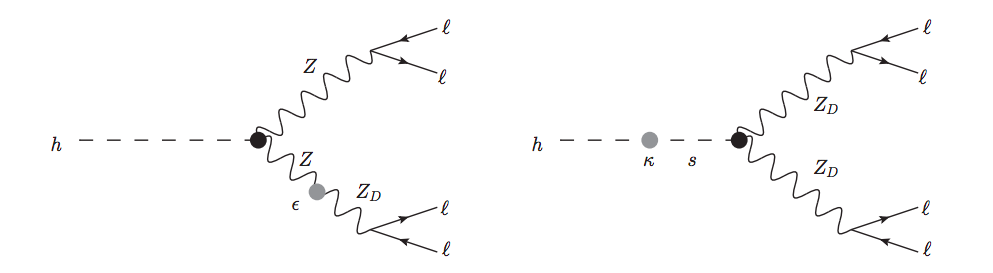
\includegraphics [width=0.75\textwidth] {Figures/Model/zdfeyn}}
\caption{
Exotic Higgs decays to four leptons via intermediate dark photons in the hypercharge portal (left) and Higgs portal (right).
}
\label{fig:feyn_zd}
\end{center}
\end{figure}

\section{Datasets}
\label{sec:datamc}

\subsection{Data}

\subsubsection{Triggers and Datasets}
\label{sec:trigpaths}


This analysis uses data samples recorded by the CMS experiment during Run 2, corresponding to $\usedLumi$ of data.  
%The HLT paths used for 2016 collision data are listed in Table~\ref{tab:triggerPaths}. 
The HLT paths used for the collision data are listed in Table~\ref{tab:triggerPaths_16}-~\ref{tab:triggerPaths_17}. 
The datasets are listed in Table~\ref{tab:datasets_data_16}-\ref{tab:datasets_data_18}, along with the integrated luminosity.  
The analysis relies on five different primary datasets (PDs), 
{\it DoubleEG}, {\it DoubleMuon}, {\it MuEG}, {\it SingleElectron}, and {\it SingleMuon},
each of which combines a certain collections of HLT paths. 
To avoid duplicate events from different primary datasets, events are taken:
\begin{itemize}
\item from DoubleEG if they pass the diEle or triEle triggers,
\item from DoubleMuon if they pass the diMuon or triMuon triggers and fail the diEle and triEle triggers,
\item from MuEG if they pass the MuEle or MuDiEle or DiMuEle triggers and fail the diEle, triEle, diMuon and triMuon triggers,
\item from SingleElectron if they pass the singleElectron trigger and fail all the above triggers. 
\item from SingleMuon if they pass the singleMuon trigger and fail all the above triggers. 
\end{itemize} 

\begin{table}[h]
\scriptsize
    \centering
    \begin{tabular}{|l|l|l|} 
\hline %----------------------------------------------------------------------------------------
\hline %---------------------------------------------------------------------------------------- 
Run-range & Dataset & Integrated luminosity \\
\hline %----------------------------------------------------------------------------------------
\hline %---------------------------------------------------------------------------------------- 
\multirow{5}{*}{273150-275376} & /DoubleMuon/Run2016B-03Feb2017-v3/MINIAOD &  \multirow{5}{*}{$5.892\ \text{fb}^{-1}$} \\ 
& /DoubleEG/Run2016B-03Feb2017-v3/MINIAOD &  \\ 
& /MuonEG/Run2016B-03Feb2017-v3/MINIAOD &  \\ 
& /SingleElectron/Run2016B-03Feb2017-v3/MINIAOD &  \\ 
& /SingleMuon/Run2016B-03Feb2017-v3/MINIAOD &  \\ 
\hline
\multirow{5}{*}{275656-276283} & /DoubleMuon/Run2016C-03Feb2017-v1/MINIAOD &  \multirow{5}{*}{$2.646\ \text{fb}^{-1}$}  \\ 
& /DoubleEG/Run2016C-03Feb2017-v1/MINIAOD &  \\ 
& /MuonEG/Run2016C-03Feb2017-v1/MINIAOD &  \\ 
& /SingleElectron/Run2016C-03Feb2017-v1/MINIAOD &  \\ 
& /SingleMuon/Run2016C-03Feb2017-v1/MINIAOD &  \\ 
\hline
\multirow{5}{*}{276315-276811} & /DoubleMuon/Run2016D-03Feb2017-v1/MINIAOD &  \multirow{5}{*}{$4.353\ \text{fb}^{-1}$} \\ 
& /DoubleEG/Run2016D-03Feb2017-v1/MINIAOD &  \\ 
& /MuonEG/Run2016D-03Feb2017-v1/MINIAOD &  \\ 
& /SingleElectron/Run2016D-03Feb2017-v1/MINIAOD &  \\ 
& /SingleMuon/Run2016D-03Feb2017-v1/MINIAOD &  \\ 
\hline
\multirow{5}{*}{276831-277420} & /DoubleMuon/Run2016E-03Feb2017-v1/MINIAOD &  \multirow{5}{*}{$4.117\ \text{fb}^{-1}$} \\ 
& /DoubleEG/Run2016E-03Feb2017-v1/MINIAOD &  \\ 
& /MuonEG/Run2016E-03Feb2017-v1/MINIAOD &  \\ 
& /SingleElectron/Run2016E-03Feb2017-v1/MINIAOD &  \\ 
& /SingleMuon/Run2016E-03Feb2017-v1/MINIAOD &  \\ 
\hline
\multirow{5}{*}{277932-278808} & /DoubleMuon/Run2016F-03Feb2017-v1/MINIAOD &  \multirow{5}{*}{$3.186\ \text{fb}^{-1}$} \\ 
& /DoubleEG/Run2016F-03Feb2017-v1/MINIAOD &  \\ 
& /MuonEG/Run2016F-03Feb2017-v1/MINIAOD &  \\ 
& /SingleElectron/Run2016F-03Feb2017-v1/MINIAOD &  \\ 
& /SingleMuon/Run2016F-03Feb2017-v1/MINIAOD &  \\ 
\hline
\multirow{5}{*}{278820-280385} & /DoubleMuon/Run2016G-03Feb2017-v1/MINIAOD &  \multirow{5}{*}{$7.721\ \text{fb}^{-1}$} \\ 
& /DoubleEG/Run2016G-03Feb2017-v1/MINIAOD &  \\ 
& /MuonEG/Run2016G-03Feb2017-v1/MINIAOD &  \\ 
& /SingleElectron/Run2016G-03Feb2017-v1/MINIAOD &  \\ 
& /SingleMuon/Run2016G-03Feb2017-v1/MINIAOD &  \\ 
\hline
\multirow{15}{*}{281207-284068} & /DoubleMuon/Run2016H-03Feb2017\_ver2-v1/MINIAOD &  \multirow{15}{*}{$8.857\ \text{fb}^{-1}$} \\ 
& /DoubleEG/Run2016H-03Feb2017\_ver2-v1/MINIAOD   \\
& /MuonEG/Run2016H-03Feb2017\_ver2-v1/MINIAOD   \\
& /SingleElectron/Run2016H-03Feb2017\_ver2-v1/MINIAOD   \\
& /SingleMuon/Run2016H-03Feb2017\_ver2-v1/MINIAOD   \\
& /DoubleMuon/Run2016H-03Feb2017\_ver3-v1/MINIAOD   \\
& /SingleMuon/Run2016H-03Feb2017\_ver3-v1/MINIAOD   \\
& /DoubleEG/Run2016H-03Feb2017\_ver3-v1/MINIAOD   \\
& /MuonEG/Run2016H-03Feb2017\_ver3-v1/MINIAOD   \\
& /SingleElectron/Run2016H-03Feb2017\_ver3-v1/MINIAOD   \\

\hline %----------------------------------------------------------------------------------------
\hline %----------------------------------------------------------------------------------------
     \end{tabular}
\small
    \caption{ Datasets used in Run 2016. }
    \label{tab:datasets_data_16}
\end{table}

\begin{table}[h]
\scriptsize
    \centering
    \begin{tabular}{|l|l|l|} 
\hline %----------------------------------------------------------------------------------------
\hline %---------------------------------------------------------------------------------------- 
Run-range & Dataset & Integrated luminosity \\
\hline %----------------------------------------------------------------------------------------
\hline %---------------------------------------------------------------------------------------- 
\multirow{5}{*}{297046-299329} & /DoubleMuon/Run2017B-17Nov2017-v1/MINIAOD &  \multirow{5}{*}{$4.792\ \text{fb}^{-1}$} \\ 
& /DoubleEG/Run2017B-17Nov2017-v1/MINIAOD &  \\ 
& /MuonEG/Run2017B-17Nov2017-v1/MINIAOD &  \\ 
& /SingleElectron/Run2017B-17Nov2017-v1/MINIAOD &  \\ 
& /SingleMuon/Run2017B-17Nov2017-v1/MINIAOD &  \\ 
\hline
\multirow{5}{*}{299368-300676} & /DoubleMuon/Run2017C-17Nov2017-v1/MINIAOD &  \multirow{5}{*}{$9.755\ \text{fb}^{-1}$}  \\ 
& /DoubleEG/Run2017C-17Nov2017-v1/MINIAOD &  \\ 
& /MuonEG/Run2017C-17Nov2017-v1/MINIAOD &  \\ 
& /SingleElectron/Run2017C-17Nov2017-v1/MINIAOD &  \\ 
& /SingleMuon/Run2017C-17Nov2017-v1/MINIAOD &  \\ 
\hline
\multirow{5}{*}{302030-303434} & /DoubleMuon/Run2017D-17Nov2017-v1/MINIAOD &  \multirow{5}{*}{$4.319\ \text{fb}^{-1}$} \\ 
& /DoubleEG/Run2017D-17Nov2017-v1/MINIAOD &  \\ 
& /MuonEG/Run2017D-17Nov2017-v1/MINIAOD &  \\ 
& /SingleElectron/Run2017D-17Nov2017-v1/MINIAOD &  \\ 
& /SingleMuon/Run2017D-17Nov2017-v1/MINIAOD &  \\ 
\hline
\multirow{5}{*}{303824-304797} & /DoubleMuon/Run2017E-17Nov2017-v1/MINIAOD &  \multirow{5}{*}{$9.424\ \text{fb}^{-1}$} \\ 
& /DoubleEG/Run2017E-17Nov2017-v1/MINIAOD &  \\ 
& /MuonEG/Run2017E-17Nov2017-v1/MINIAOD &  \\ 
& /SingleElectron/Run2017E-17Nov2017-v1/MINIAOD &  \\ 
& /SingleMuon/Run2017E-17Nov2017-v1/MINIAOD &  \\ 
\hline
\multirow{5}{*}{305040-306462} & /DoubleMuon/Run2017F-17Nov2017-v1/MINIAOD &  \multirow{5}{*}{$13.50\ \text{fb}^{-1}$} \\ 
& /DoubleEG/Run2017F-17Nov2017-v1/MINIAOD &  \\ 
& /MuonEG/Run2017F-17Nov2017-v1/MINIAOD &  \\ 
& /SingleElectron/Run2017F-17Nov2017-v1/MINIAOD &  \\ 
& /SingleMuon/Run2017F-17Nov2017-v1/MINIAOD &  \\ 
\hline
\hline %----------------------------------------------------------------------------------------
\hline %----------------------------------------------------------------------------------------
     \end{tabular}
\small
    \caption{ Datasets used in Run 2017. }
    \label{tab:datasets_data_17}
\end{table}

\begin{table}[h]
\scriptsize
    \centering
    \begin{tabular}{|l|l|l|} 
\hline %----------------------------------------------------------------------------------------
\hline %---------------------------------------------------------------------------------------- 
Run-range & Dataset & Integrated luminosity \\
\hline %----------------------------------------------------------------------------------------
\hline %---------------------------------------------------------------------------------------- 
\multirow{5}{*}{297046-299329} & /DoubleMuon/Run2017B-17Nov2017-v1/MINIAOD &  \multirow{5}{*}{$4.792\ \text{fb}^{-1}$} \\ 
& /DoubleEG/Run2017B-17Nov2017-v1/MINIAOD &  \\ 
& /MuonEG/Run2017B-17Nov2017-v1/MINIAOD &  \\ 
& /SingleElectron/Run2017B-17Nov2017-v1/MINIAOD &  \\ 
& /SingleMuon/Run2017B-17Nov2017-v1/MINIAOD &  \\ 
\hline
\multirow{5}{*}{299368-300676} & /DoubleMuon/Run2017C-17Nov2017-v1/MINIAOD &  \multirow{5}{*}{$9.755\ \text{fb}^{-1}$}  \\ 
& /DoubleEG/Run2017C-17Nov2017-v1/MINIAOD &  \\ 
& /MuonEG/Run2017C-17Nov2017-v1/MINIAOD &  \\ 
& /SingleElectron/Run2017C-17Nov2017-v1/MINIAOD &  \\ 
& /SingleMuon/Run2017C-17Nov2017-v1/MINIAOD &  \\ 
\hline
\multirow{5}{*}{302030-303434} & /DoubleMuon/Run2017D-17Nov2017-v1/MINIAOD &  \multirow{5}{*}{$4.319\ \text{fb}^{-1}$} \\ 
& /DoubleEG/Run2017D-17Nov2017-v1/MINIAOD &  \\ 
& /MuonEG/Run2017D-17Nov2017-v1/MINIAOD &  \\ 
& /SingleElectron/Run2017D-17Nov2017-v1/MINIAOD &  \\ 
& /SingleMuon/Run2017D-17Nov2017-v1/MINIAOD &  \\ 
\hline
\multirow{5}{*}{303824-304797} & /DoubleMuon/Run2017E-17Nov2017-v1/MINIAOD &  \multirow{5}{*}{$9.424\ \text{fb}^{-1}$} \\ 
& /DoubleEG/Run2017E-17Nov2017-v1/MINIAOD &  \\ 
& /MuonEG/Run2017E-17Nov2017-v1/MINIAOD &  \\ 
& /SingleElectron/Run2017E-17Nov2017-v1/MINIAOD &  \\ 
& /SingleMuon/Run2017E-17Nov2017-v1/MINIAOD &  \\ 
\hline
\multirow{5}{*}{305040-306462} & /DoubleMuon/Run2017F-17Nov2017-v1/MINIAOD &  \multirow{5}{*}{$13.50\ \text{fb}^{-1}$} \\ 
& /DoubleEG/Run2017F-17Nov2017-v1/MINIAOD &  \\ 
& /MuonEG/Run2017F-17Nov2017-v1/MINIAOD &  \\ 
& /SingleElectron/Run2017F-17Nov2017-v1/MINIAOD &  \\ 
& /SingleMuon/Run2017F-17Nov2017-v1/MINIAOD &  \\ 
\hline
\hline %----------------------------------------------------------------------------------------
\hline %----------------------------------------------------------------------------------------
     \end{tabular}
\small
\caption{ [Placehoder for 2018] Datasets used in the analysis. }
    \label{tab:datasets_data_18}
\end{table}


\begin{table}[h]
\scriptsize
    \centering
    \begin{tabular}{|l|l|c|l|} 
\hline %--------------------------------------------------------------------------------------------------------------------------
HLT path                      				       & L1 seed                          & prescale  & primary dataset \\
\hline %--------------------------------------------------------------------------------------------------------------------------
\verb| HLT_Ele17_Ele12_CaloIdL_TrackIdL_IsoVL_DZ       | & \verb| L1_DoubleEG_15_10    |  & 1 & DoubleEG \\
\verb| HLT_Ele23_Ele12_CaloIdL_TrackIdL_IsoVL_DZ       | & \verb| L1_DoubleEG_22_10    |  & 1 & DoubleEG \\
\verb| HLT_DoubleEle33_CaloIdL_GsfTrkIdVL              | & \verb| (Multiple)           |  & 1 & DoubleEG \\
\verb| HLT_Ele16_Ele12_Ele8_CaloIdL_TrackIdL           | & \verb| L1_TripleEG_14_10_8  |  & 1 & DoubleEG \\
\verb| HLT_Mu17_TrkIsoVVL_Mu8_TrkIsoVVL                | & \verb| L1_DoubleMu_11_4     |  & 1 & DoubleMuon \\
\verb| HLT_Mu17_TrkIsoVVL_TkMu8_TrkIsoVVL              | & \verb| L1_DoubleMu_11_4     |  & 1 & DoubleMuon \\
\verb| HLT_TripleMu_12_10_5                            | & \verb| L1_TripleMu_5_5_3    |  & 1 & DoubleMuon \\
\verb| HLT_Mu8_TrkIsoVVL_Ele17_CaloIdL_TrackIdL_IsoVL  | & \verb| L1_Mu5_EG15          |  & 1 & MuonEG \\
\verb| HLT_Mu8_TrkIsoVVL_Ele23_CaloIdL_TrackIdL_IsoVL  | & \verb| L1_Mu5_EG20          |  & 1 & MuonEG \\
\verb| HLT_Mu17_TrkIsoVVL_Ele12_CaloIdL_TrackIdL_IsoVL | & \verb| L1_Mu12_EG10         |  & 1 & MuonEG \\
\verb| HLT_Mu23_TrkIsoVVL_Ele12_CaloIdL_TrackIdL_IsoVL | & \verb| L1_Mu20_EG10         |  & 1 & MuonEG \\
\verb| HLT_Mu23_TrkIsoVVL_Ele8_CaloIdL_TrackIdL_IsoVL  | & \verb| L1_SingleMu*         |  & 1 & MuonEG \\
\verb| HLT_Mu8_DiEle12_CaloIdL_TrackIdL                | & \verb| L1_Mu6_DoubleEG10    |  & 1 & MuonEG \\
\verb| HLT_DiMu9_Ele9_CaloIdL_TrackIdL                 | & \verb| L1_DoubleMu7_EG7     |  & 1 & MuonEG \\
\verb| HLT_Ele25_eta2p1_WPTight                        | & \verb| L1_SingleEG*         |  & 1 & SingleElectron \\
\verb| HLT_Ele27_WPTight                               | & \verb| L1_SingleEG*         |  & 1 & SingleElectron \\
\verb| HLT_Ele27_eta2p1_WPLoose_Gsf                    | & \verb| L1_SingleEG*         |  & 1 & SingleElectron \\
\verb| HLT_IsoMu20 OR HLT_IsoTkMu20                    | & \verb| L1_SingleMu*         |  & 1 & SingleMuon \\
\verb| HLT_IsoMu22 OR HLT_IsoTkMu22                    | & \verb| L1_SingleMu*         |  & 1 & SingleMuon \\
\hline %--------------------------------------------------------------------------------------------------------------------------
    \end{tabular}
\small
    \caption{Trigger paths used in 2016 collision data.}
    \label{tab:triggerPaths_16}
\end{table}

\begin{table}[h]
\scriptsize
    \centering
    \begin{tabular}{|l|l|c|l|} 
\hline %--------------------------------------------------------------------------------------------------------------------------
HLT path                      				       & L1 seed                          & prescale  & primary dataset \\
\hline %--------------------------------------------------------------------------------------------------------------------------
\verb| HLT_Ele23_Ele12_CaloIdL_TrackIdL_IsoVL_*        | & \verb| L1_DoubleEG_22_10    |  & 1 & DoubleEG \\
\verb| HLT_DoubleEle33_CaloIdL_GsfTrkIdVL              | & \verb| (Multiple)           |  & 1 & DoubleEG \\
\verb| HLT_Ele16_Ele12_Ele8_CaloIdL_TrackIdL           | & \verb| L1_TripleEG_14_10_8  |  & 1 & DoubleEG \\
\verb| HLT_Mu17_TrkIsoVVL_Mu8_TrkIsoVVL_DZ_Mass3p8     | & \verb| L1_DoubleMu_11_4     |  & 1 & DoubleMuon \\
\verb| HLT_Mu17_TrkIsoVVL_Mu8_TrkIsoVVL_DZ_Mass8       | & \verb| L1_DoubleMu_11_4     |  & 1 & DoubleMuon \\
\verb| HLT_TripleMu_12_10_5                            | & \verb| L1_TripleMu_5_5_3    |  & 1 & DoubleMuon \\
\verb| HLT_TripleMu_10_5_5_D2                          | & \verb| L1_TripleMu_5_5_3    |  & 1 & DoubleMuon \\
\verb| HLT_Mu23_TrkIsoVVL_Ele12_CaloIdL_TrackIdL_IsoVL | & \verb| L1_XX | & 1 & MuonEG \\
\verb| HLT_Mu8_TrkIsoVVL_Ele23_CaloIdL_TrackIdL_IsoVL_DZ | & \verb| L1_XX | & 1 & MuonEG \\
\verb| HLT_Mu12_TrkIsoVVL_Ele23_CaloIdL_TrackIdL_IsoVL_DZ| & \verb| L1_XX | & 1 & MuonEG \\
\verb| HLT_Mu23_TrkIsoVVL_Ele12_CaloIdL_TrackIdL_IsoVL_DZ| & \verb| L1_XX | & 1 & MuonEG \\
\verb| HLT_DiMu9_Ele9_CaloIdL_TrackIdL_DZ| & \verb| L1_XX | & 1 & MuonEG \\
\verb| HLT_Mu8_DiEle12_CaloIdL_TrackIdL | & \verb| L1_XX | & 1 & MuonEG \\
\verb| HLT_Mu8_DiEle12_CaloIdL_TrackIdL_DZ | & \verb| L1_XX | & 1 & MuonEG \\
\verb| HLT_Ele35_WPTight_Gsf_v*                        | & \verb| L1_EG* | & 1 & SingleElectron \\
\verb| HLT_Ele38_WPTight_Gsf_v*                        | & \verb| L1_EG* | & 1 & SingleElectron \\
\verb| HLT_Ele40_WPTight_Gsf_v*                        | & \verb| L1_EG* | & 1 & SingleElectron \\
\verb| HLT_IsoMu27                                     | & \verb| L1_SingleMu*         |  & 1 & SingleMuon \\
\hline %--------------------------------------------------------------------------------------------------------------------------
    \end{tabular}
\small
    \caption{Trigger paths used in 2017 collision data.}
    \label{tab:triggerPaths_17}
\end{table}

\begin{table}[h]
\scriptsize
    \centering
    \begin{tabular}{|l|l|c|l|} 
\hline %--------------------------------------------------------------------------------------------------------------------------
HLT path                      				       & L1 seed                          & prescale  & primary dataset \\
\hline %--------------------------------------------------------------------------------------------------------------------------
\verb| HLT_Ele23_Ele12_CaloIdL_TrackIdL_IsoVL_*        | & \verb| L1_DoubleEG_22_10    |  & 1 & DoubleEG \\
\verb| HLT_DoubleEle33_CaloIdL_GsfTrkIdVL              | & \verb| (Multiple)           |  & 1 & DoubleEG \\
\verb| HLT_Ele16_Ele12_Ele8_CaloIdL_TrackIdL           | & \verb| L1_TripleEG_14_10_8  |  & 1 & DoubleEG \\
\verb| HLT_Mu17_TrkIsoVVL_Mu8_TrkIsoVVL_DZ_Mass3p8     | & \verb| L1_DoubleMu_11_4     |  & 1 & DoubleMuon \\
\verb| HLT_Mu17_TrkIsoVVL_Mu8_TrkIsoVVL_DZ_Mass8       | & \verb| L1_DoubleMu_11_4     |  & 1 & DoubleMuon \\
\verb| HLT_TripleMu_12_10_5                            | & \verb| L1_TripleMu_5_5_3    |  & 1 & DoubleMuon \\
\verb| HLT_TripleMu_10_5_5_D2                          | & \verb| L1_TripleMu_5_5_3    |  & 1 & DoubleMuon \\
\verb| HLT_Mu23_TrkIsoVVL_Ele12_CaloIdL_TrackIdL_IsoVL | & \verb| L1_XX | & 1 & MuonEG \\
\verb| HLT_Mu8_TrkIsoVVL_Ele23_CaloIdL_TrackIdL_IsoVL_DZ | & \verb| L1_XX | & 1 & MuonEG \\
\verb| HLT_Mu12_TrkIsoVVL_Ele23_CaloIdL_TrackIdL_IsoVL_DZ| & \verb| L1_XX | & 1 & MuonEG \\
\verb| HLT_Mu23_TrkIsoVVL_Ele12_CaloIdL_TrackIdL_IsoVL_DZ| & \verb| L1_XX | & 1 & MuonEG \\
\verb| HLT_DiMu9_Ele9_CaloIdL_TrackIdL_DZ| & \verb| L1_XX | & 1 & MuonEG \\
\verb| HLT_Mu8_DiEle12_CaloIdL_TrackIdL | & \verb| L1_XX | & 1 & MuonEG \\
\verb| HLT_Mu8_DiEle12_CaloIdL_TrackIdL_DZ | & \verb| L1_XX | & 1 & MuonEG \\
\verb| HLT_Ele35_WPTight_Gsf_v*                        | & \verb| L1_EG* | & 1 & SingleElectron \\
\verb| HLT_Ele38_WPTight_Gsf_v*                        | & \verb| L1_EG* | & 1 & SingleElectron \\
\verb| HLT_Ele40_WPTight_Gsf_v*                        | & \verb| L1_EG* | & 1 & SingleElectron \\
\verb| HLT_IsoMu27                                     | & \verb| L1_SingleMu*         |  & 1 & SingleMuon \\
\hline %--------------------------------------------------------------------------------------------------------------------------
    \end{tabular}
\small
\caption{[Placeholder for 2018] Trigger paths used in 2018 collision data.  }
    \label{tab:triggerPaths_18}
\end{table}

\subsubsection{Trigger Efficiency}

The efficiency in data of the combination of triggers used in the anlysis with respect to the offline reconstruction and selection is measured
by considering 4$\ell$ events triggered by single lepton triggers. One of the four reconstructed leptons ( the ``tag'') is geometrically matched 
to a trigger object passing the final filter of one of the single muon or single electron triggers. The other three leptons are 
used as ``probes''. In each 4$\ell$ event there are up to 4 possible tag-probe combinations, and all possible combinations are counted in the
denominator of the efficiency. For each of the three probe leptons all matching trigger filter objects are collected. Then the matched trigger filter
objects of the three probe leptons are combined in attempt to reconstruct any of the triggers used in the anlysis. If any of the analysis triggers
can be formed using the probe leptons, the set of probes is also counted in the numerator of the efficiency.

This method does not have a perfect closure in MC events due to the fact that the presence of a fourth lepton increases the trigger efficiency,
and this effect is not accounted for. Also, in the  $2e2\mu$ final state, the three probe leptons cannot be combined to form all possible triggers which 
can collect events with two electrons and two muons (e.g. if the tag lepton is an electron, the three remaining leptons cannot pass a double electron
trigger). Therefore the method is also exercised on MC and the difference between data and MC is used to determine the reliability of the simulation.
 The efficiency plotted as a function of the minimum $p_{\rm{T}}$ of the three probe leptons in data and MC using this method can be seen in 
 Fig.\ref{fig:TrigEff_16}-\ref{fig:TrigEff_18}. The MC efficiency describes well the data within the statistical uncertainties.

\begin{figure}[!htb]
\vspace*{0.3cm}
\begin{center}
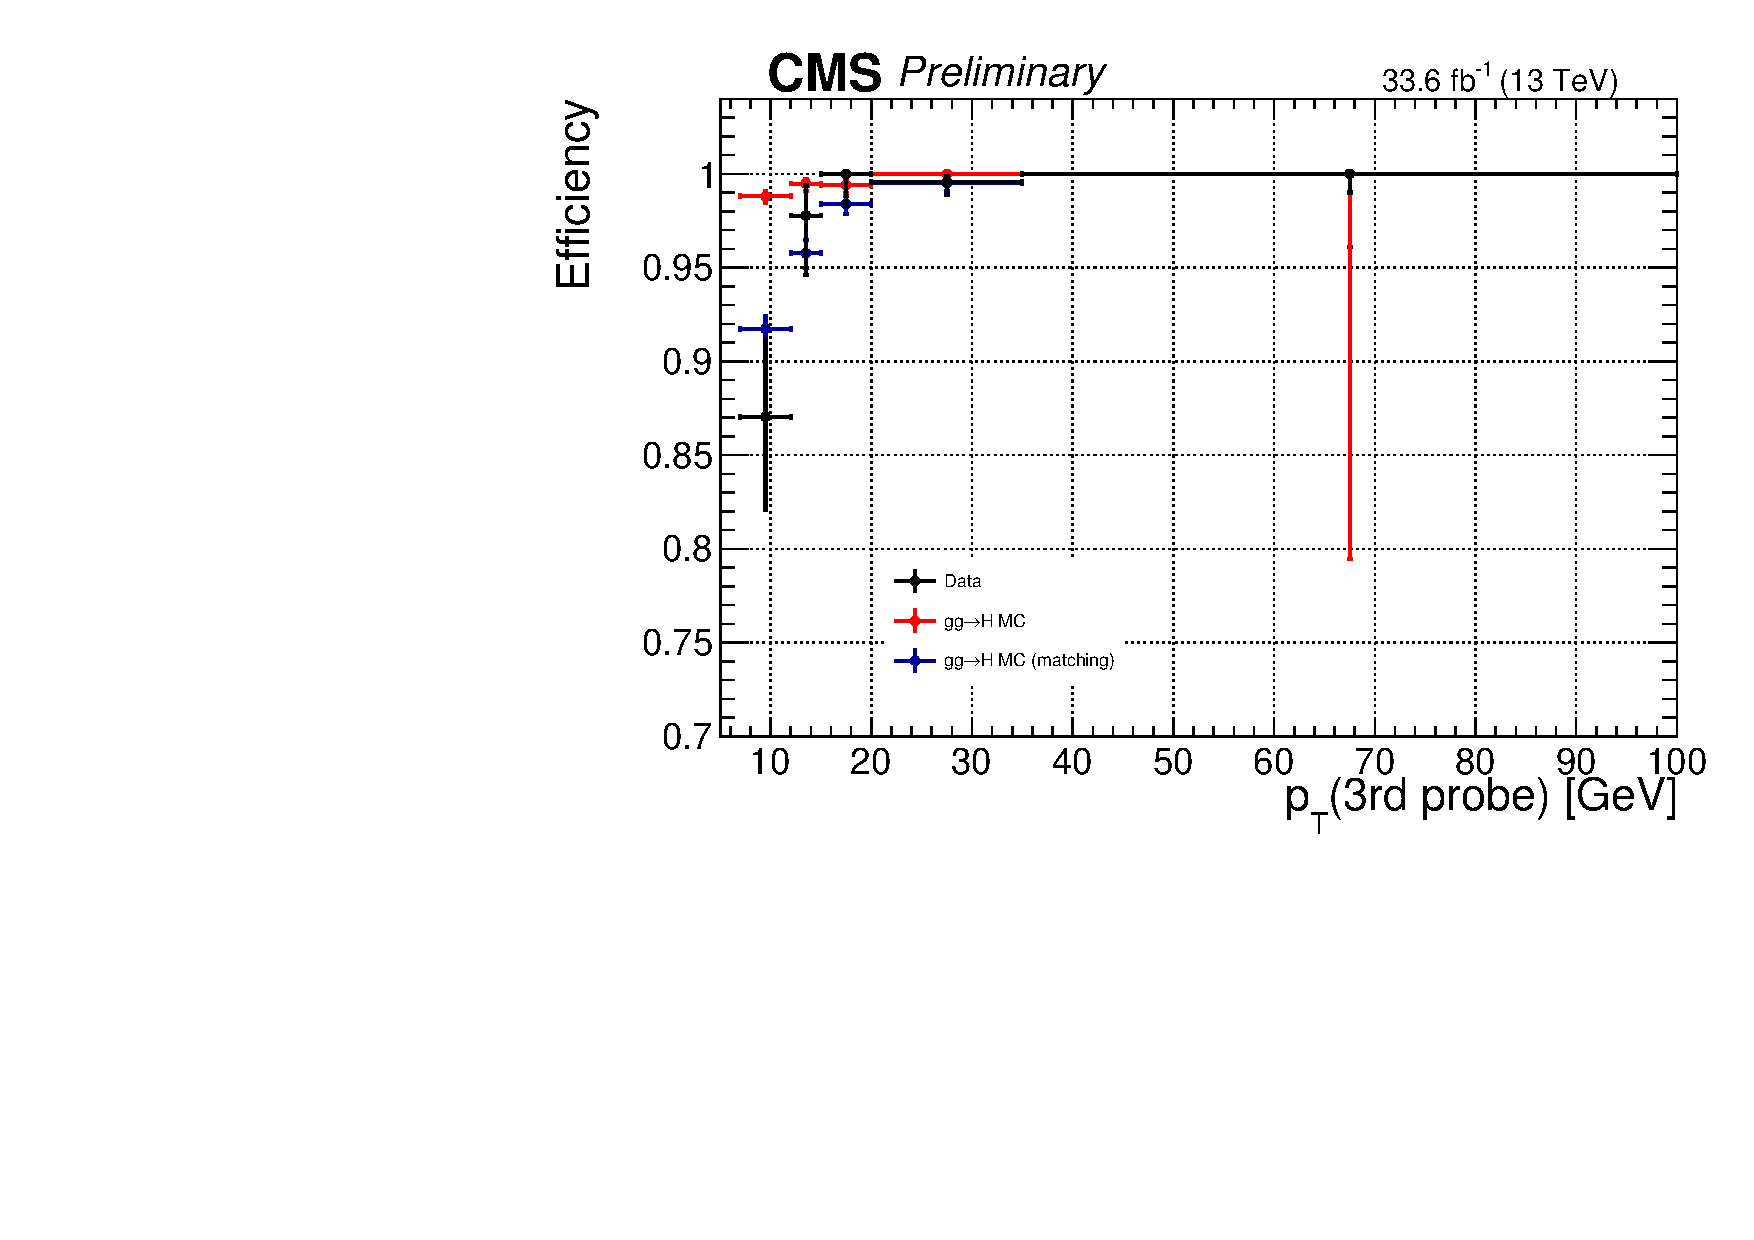
\includegraphics[width=0.45\textwidth]{Figures/Trigger16/Histo_TrigEff_ptMin_4e.pdf} 
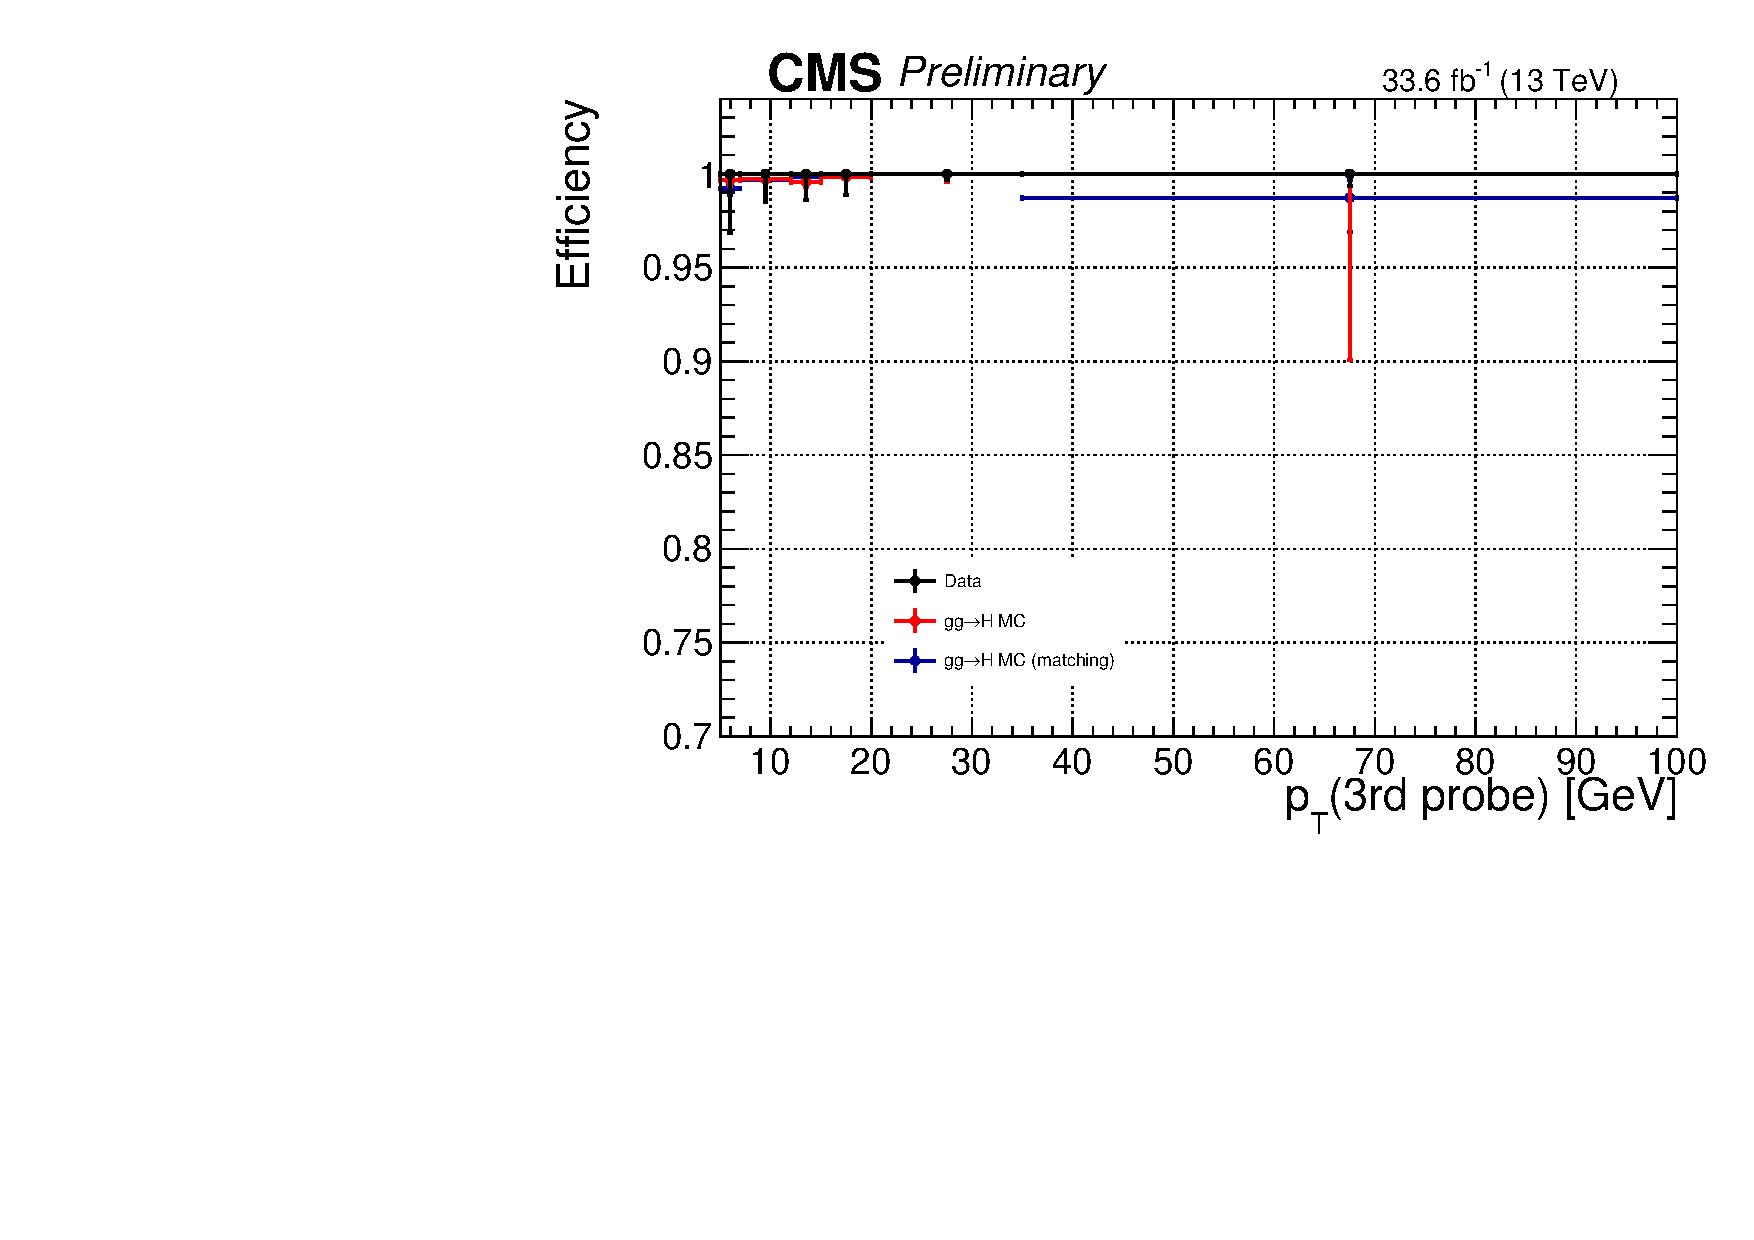
\includegraphics[width=0.45\textwidth]{Figures/Trigger16/Histo_TrigEff_ptMin_4mu.pdf} \\
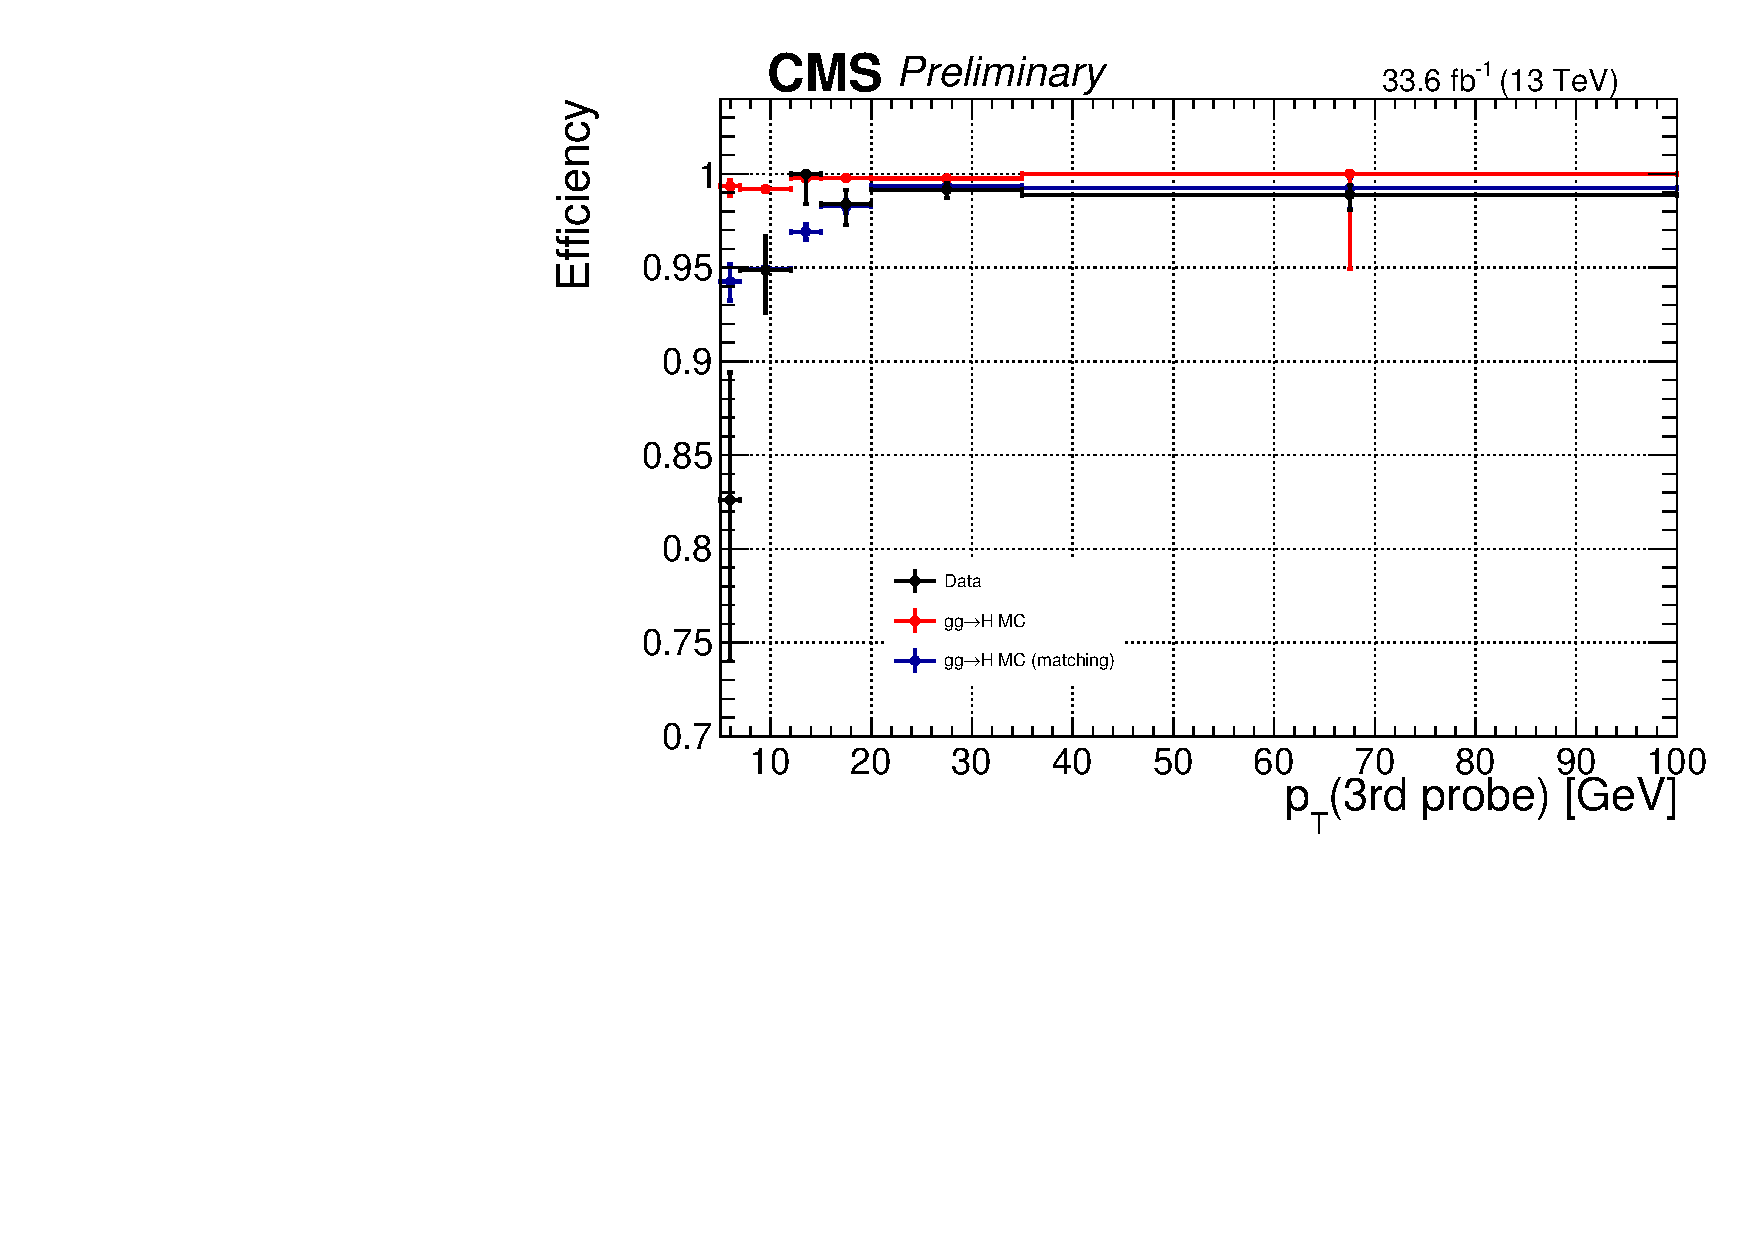
\includegraphics[width=0.45\textwidth]{Figures/Trigger16/Histo_TrigEff_ptMin_2e2mu.pdf} 
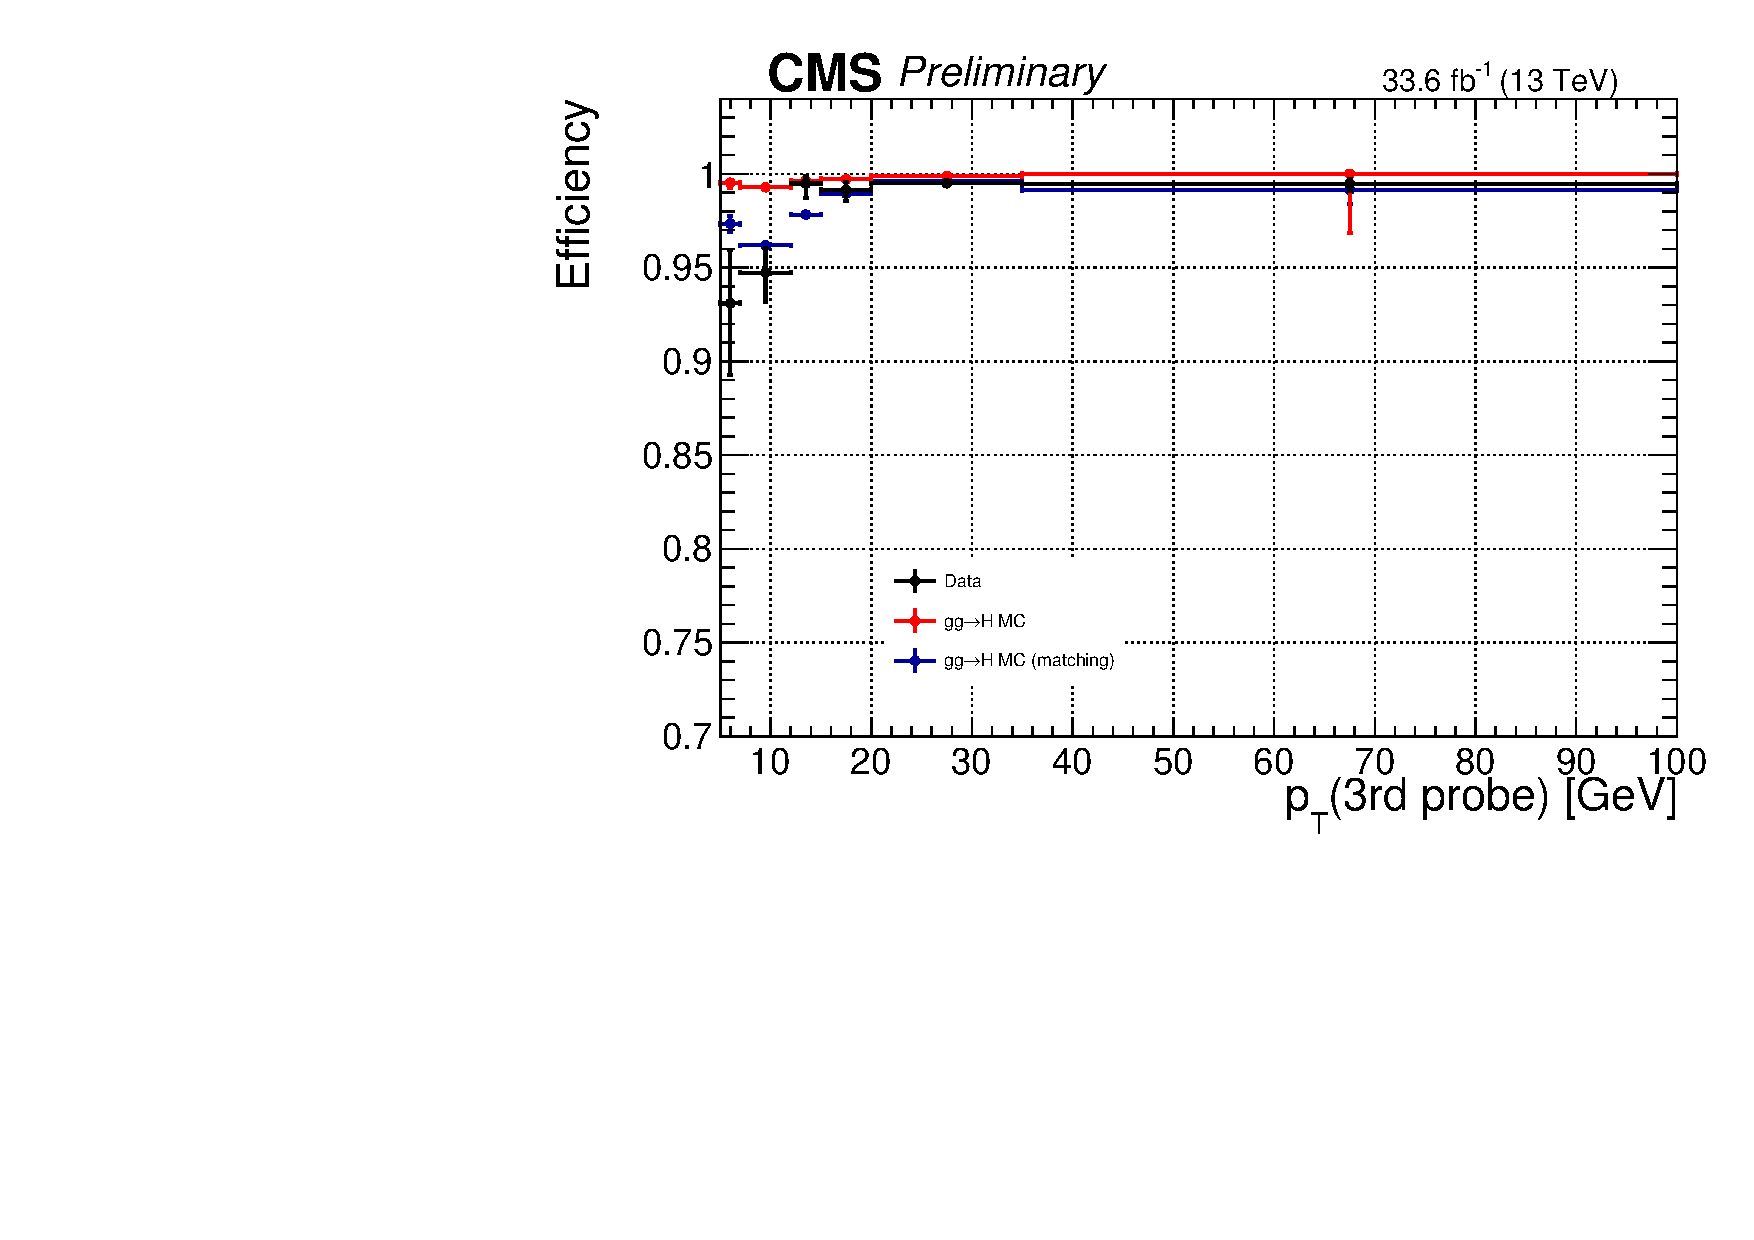
\includegraphics[width=0.45\textwidth]{Figures/Trigger16/Histo_TrigEff_ptMin_4l.pdf} \\
\caption{Trigger efficiency measured in data with Run 2016 using $4\ell$ events collected by 
    single lepton triggers for the $4e$ (top left), $4\mu$ (top right), $2e2\mu$ (bottom left) and $4\ell$ (bottom right) final states. 
%\fixme{Results using Prompt Reco, to be redone with ReReco}.
\label{fig:TrigEff_16}}
\end{center}
\end{figure}

\begin{figure}[!htb]
\vspace*{0.3cm}
\begin{center}
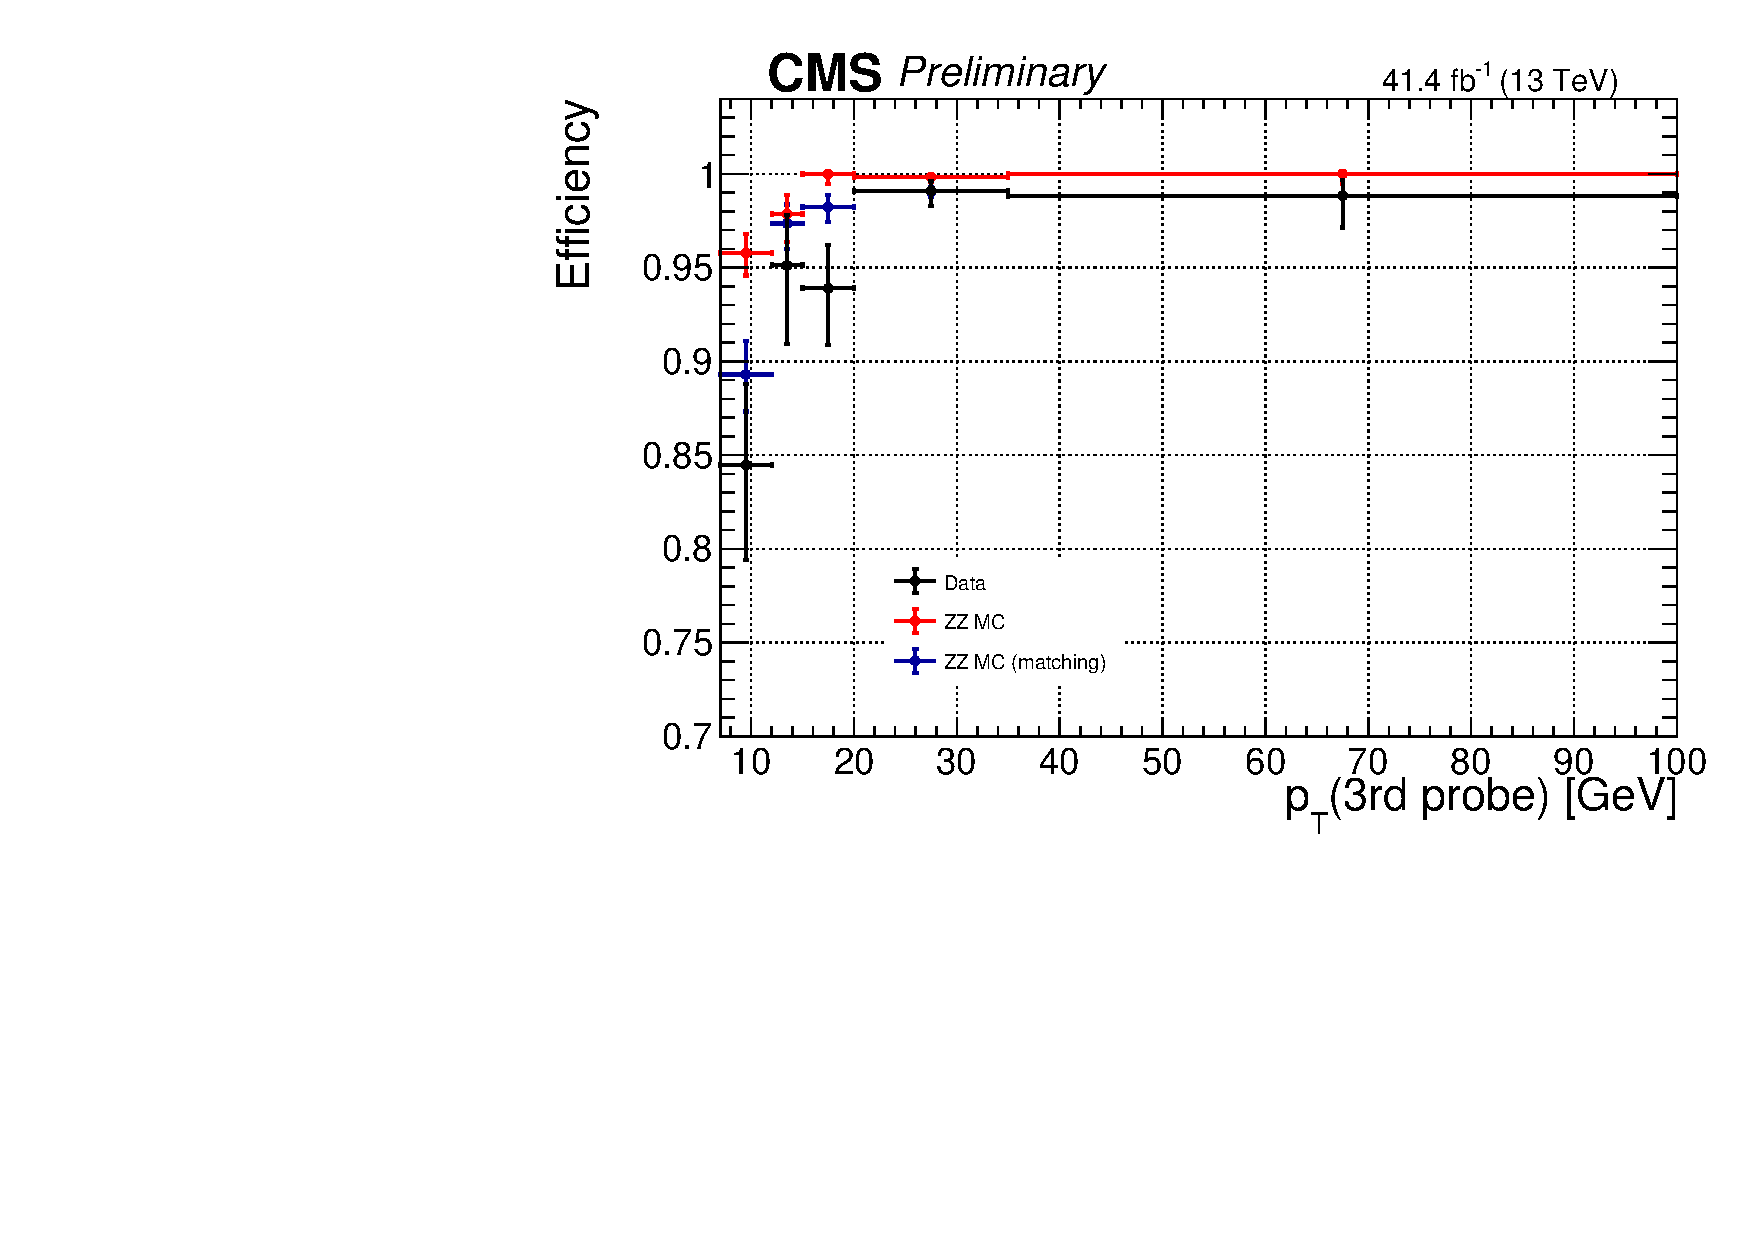
\includegraphics[width=0.45\textwidth]{Figures/Trigger17/Histo_TrigEff_ptMin_4e_mZ2_12.pdf} 
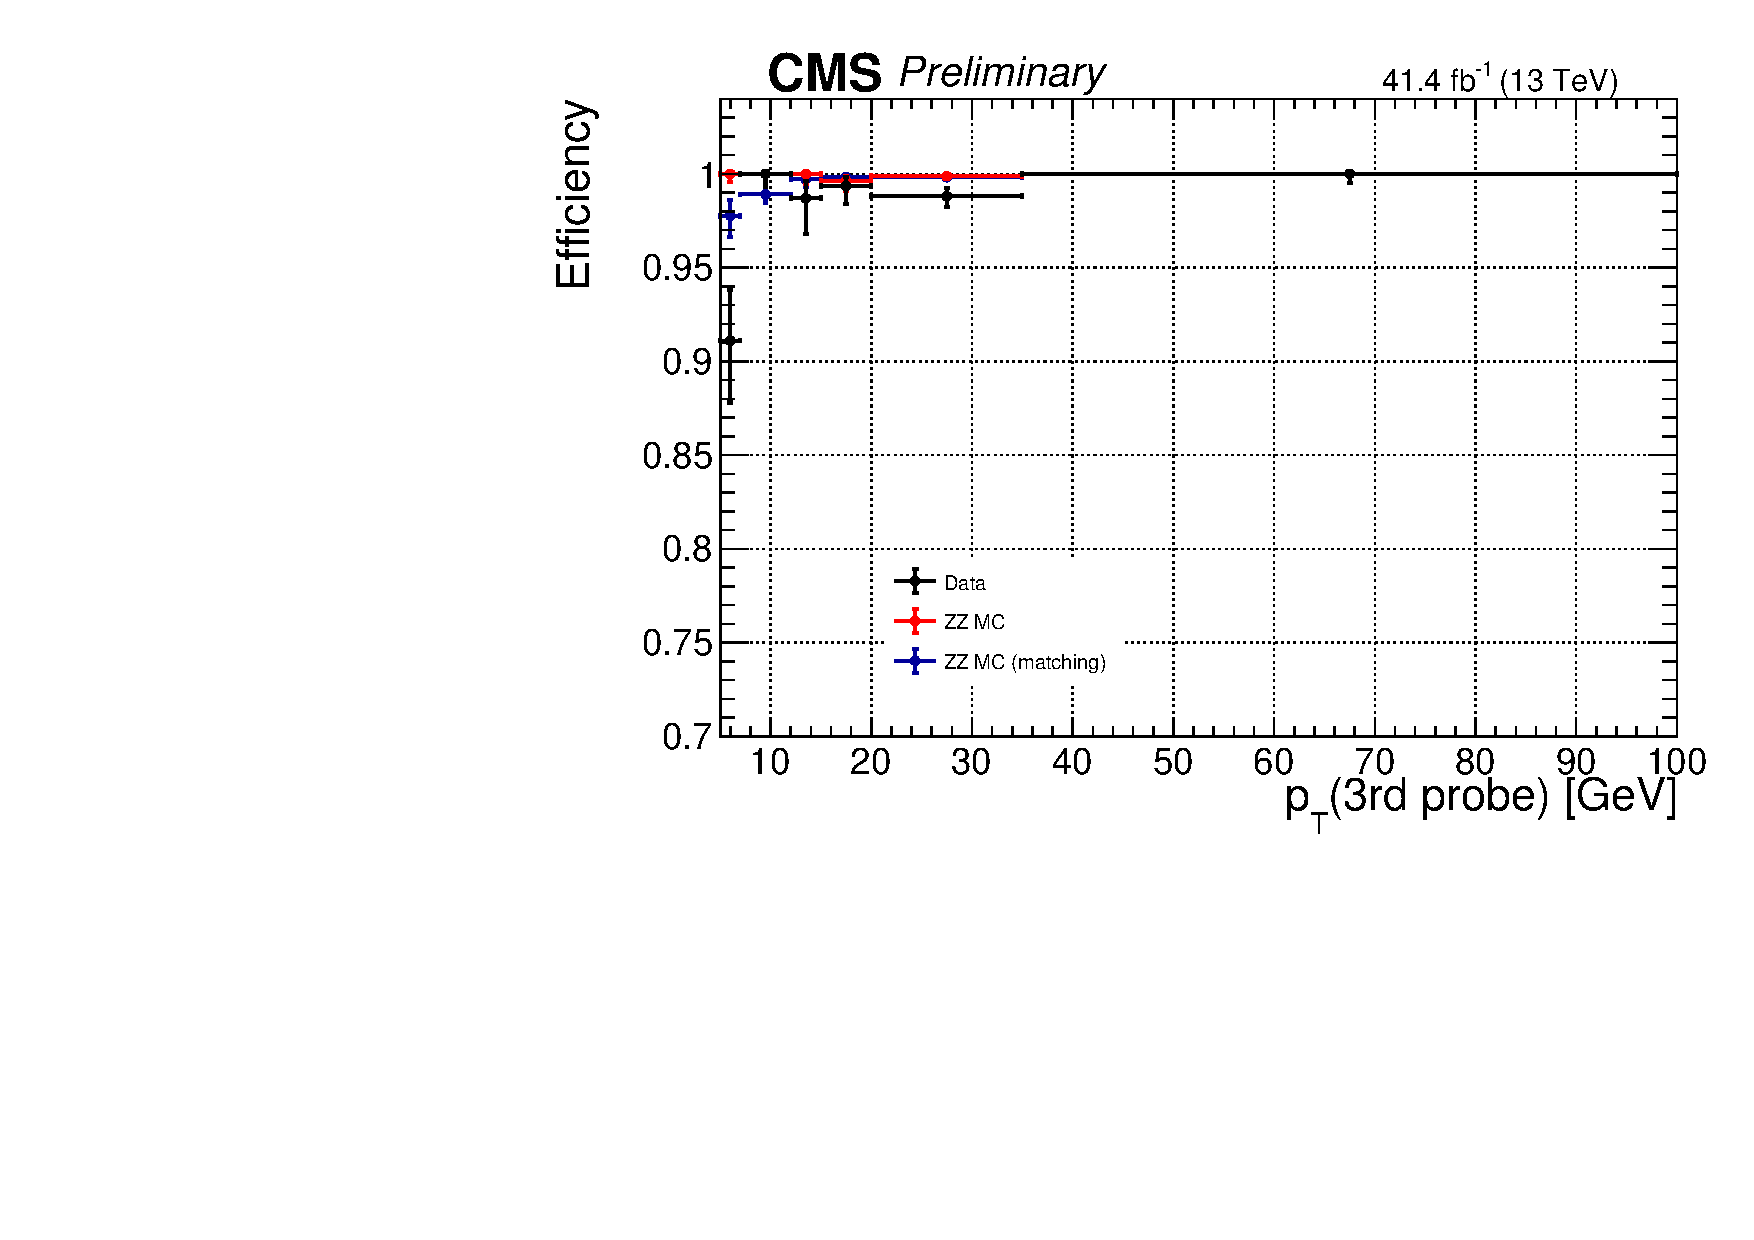
\includegraphics[width=0.45\textwidth]{Figures/Trigger17/Histo_TrigEff_ptMin_4mu_mZ2_12.pdf} \\
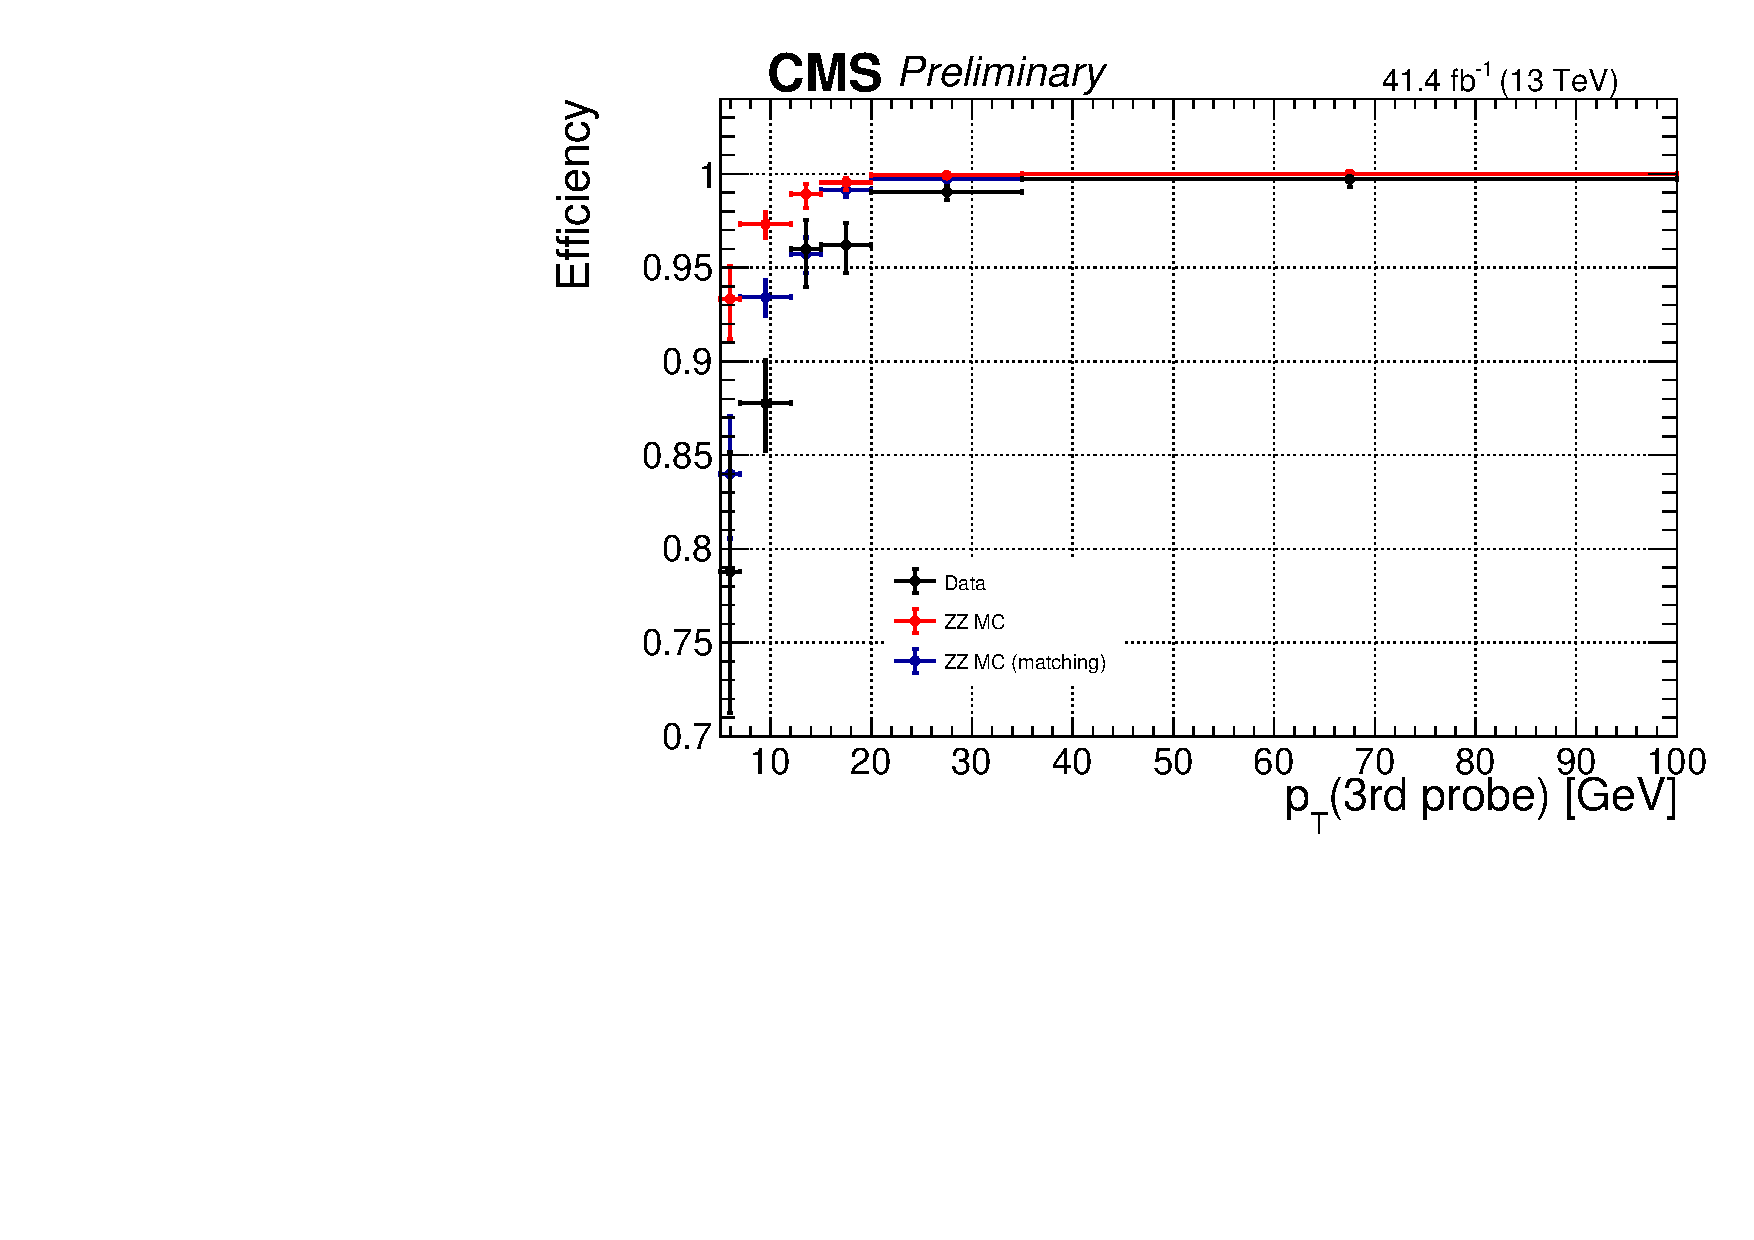
\includegraphics[width=0.45\textwidth]{Figures/Trigger17/Histo_TrigEff_ptMin_2e2mu_mZ2_12.pdf} 
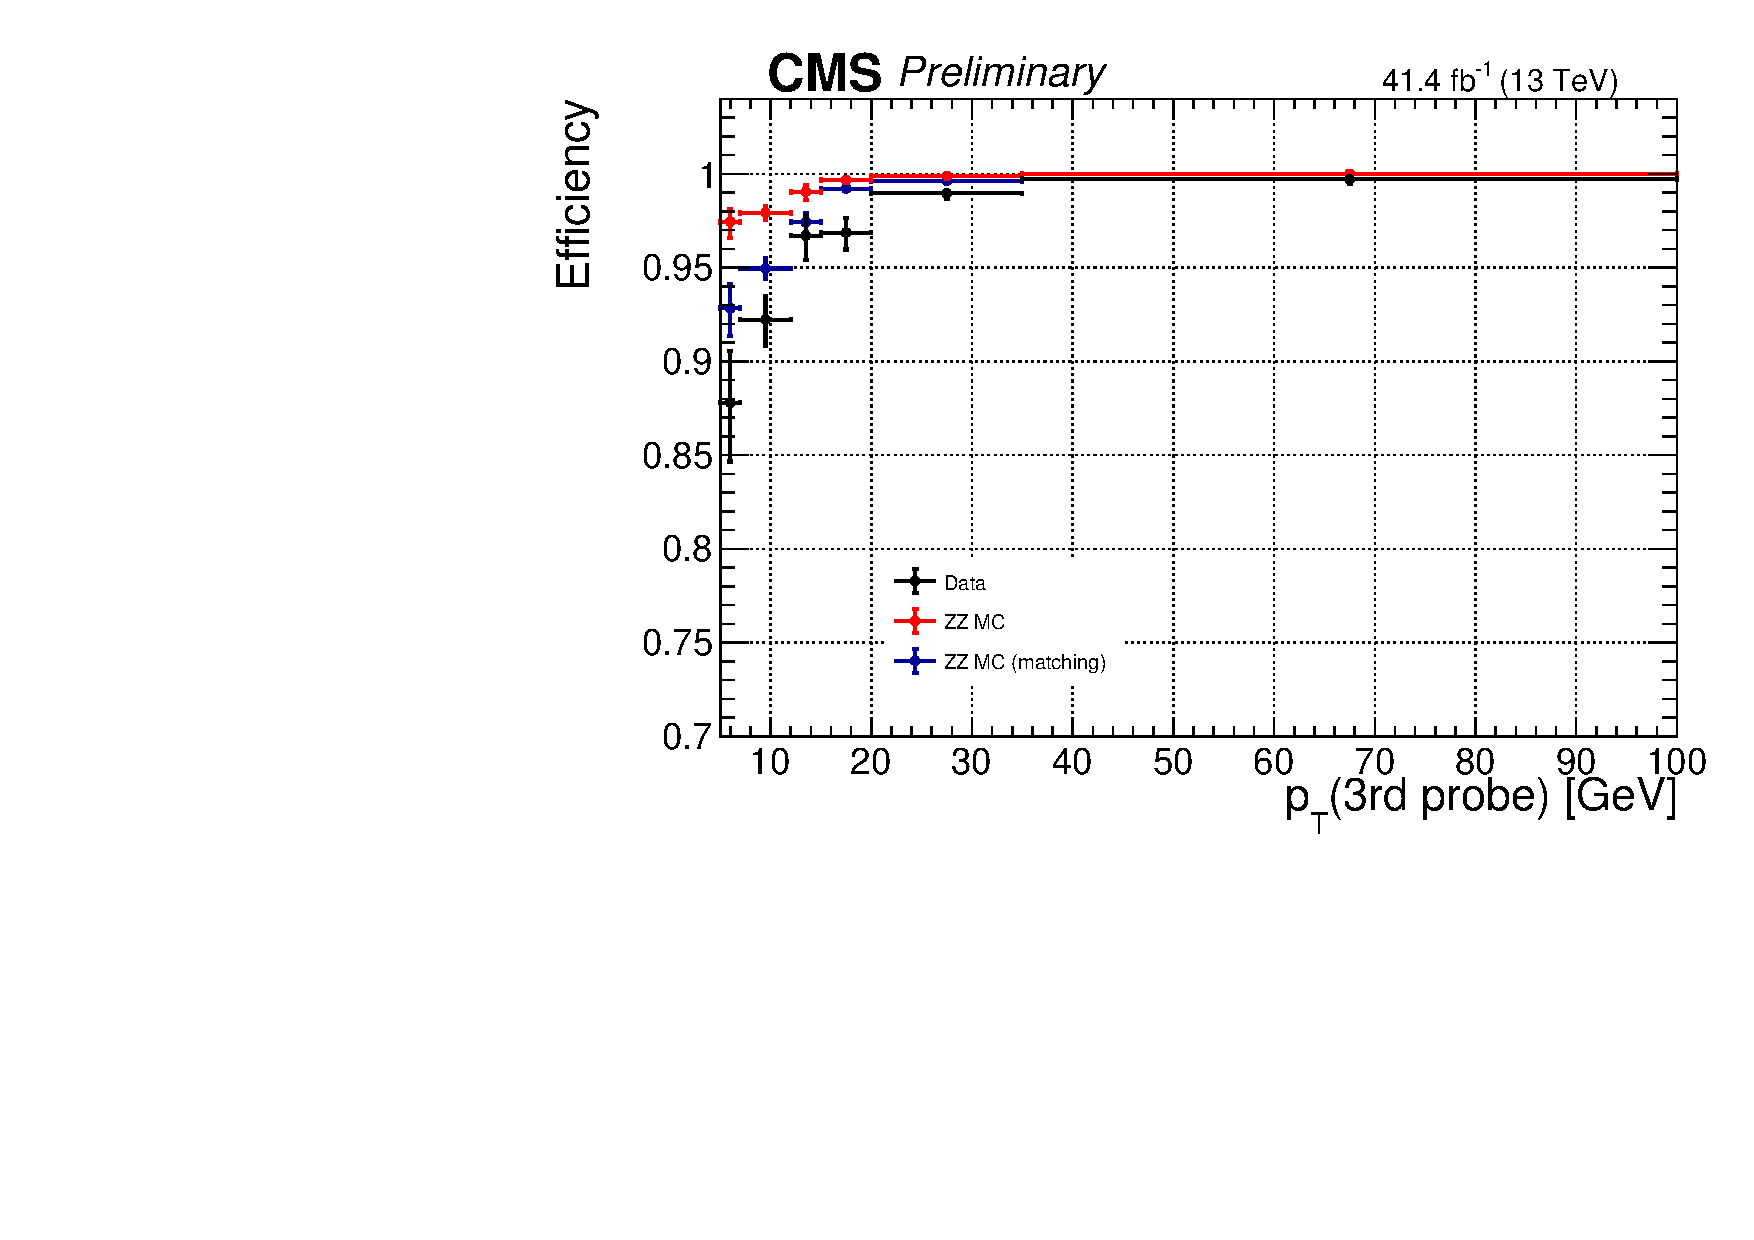
\includegraphics[width=0.45\textwidth]{Figures/Trigger17/Histo_TrigEff_ptMin_4l_mZ2_12.pdf} \\
\caption{Trigger efficiency measured in data with Run 2017 using $4\ell$ events collected by 
    single lepton triggers for the $4e$ (top left), $4\mu$ (top right), $2e2\mu$ (bottom left) and $4\ell$ (bottom right) final states. 
%\fixme{Results using Prompt Reco, to be redone with ReReco}.
\label{fig:TrigEff_17}}
\end{center}
\end{figure}

\begin{figure}[!htb]
\vspace*{0.3cm}
\begin{center}
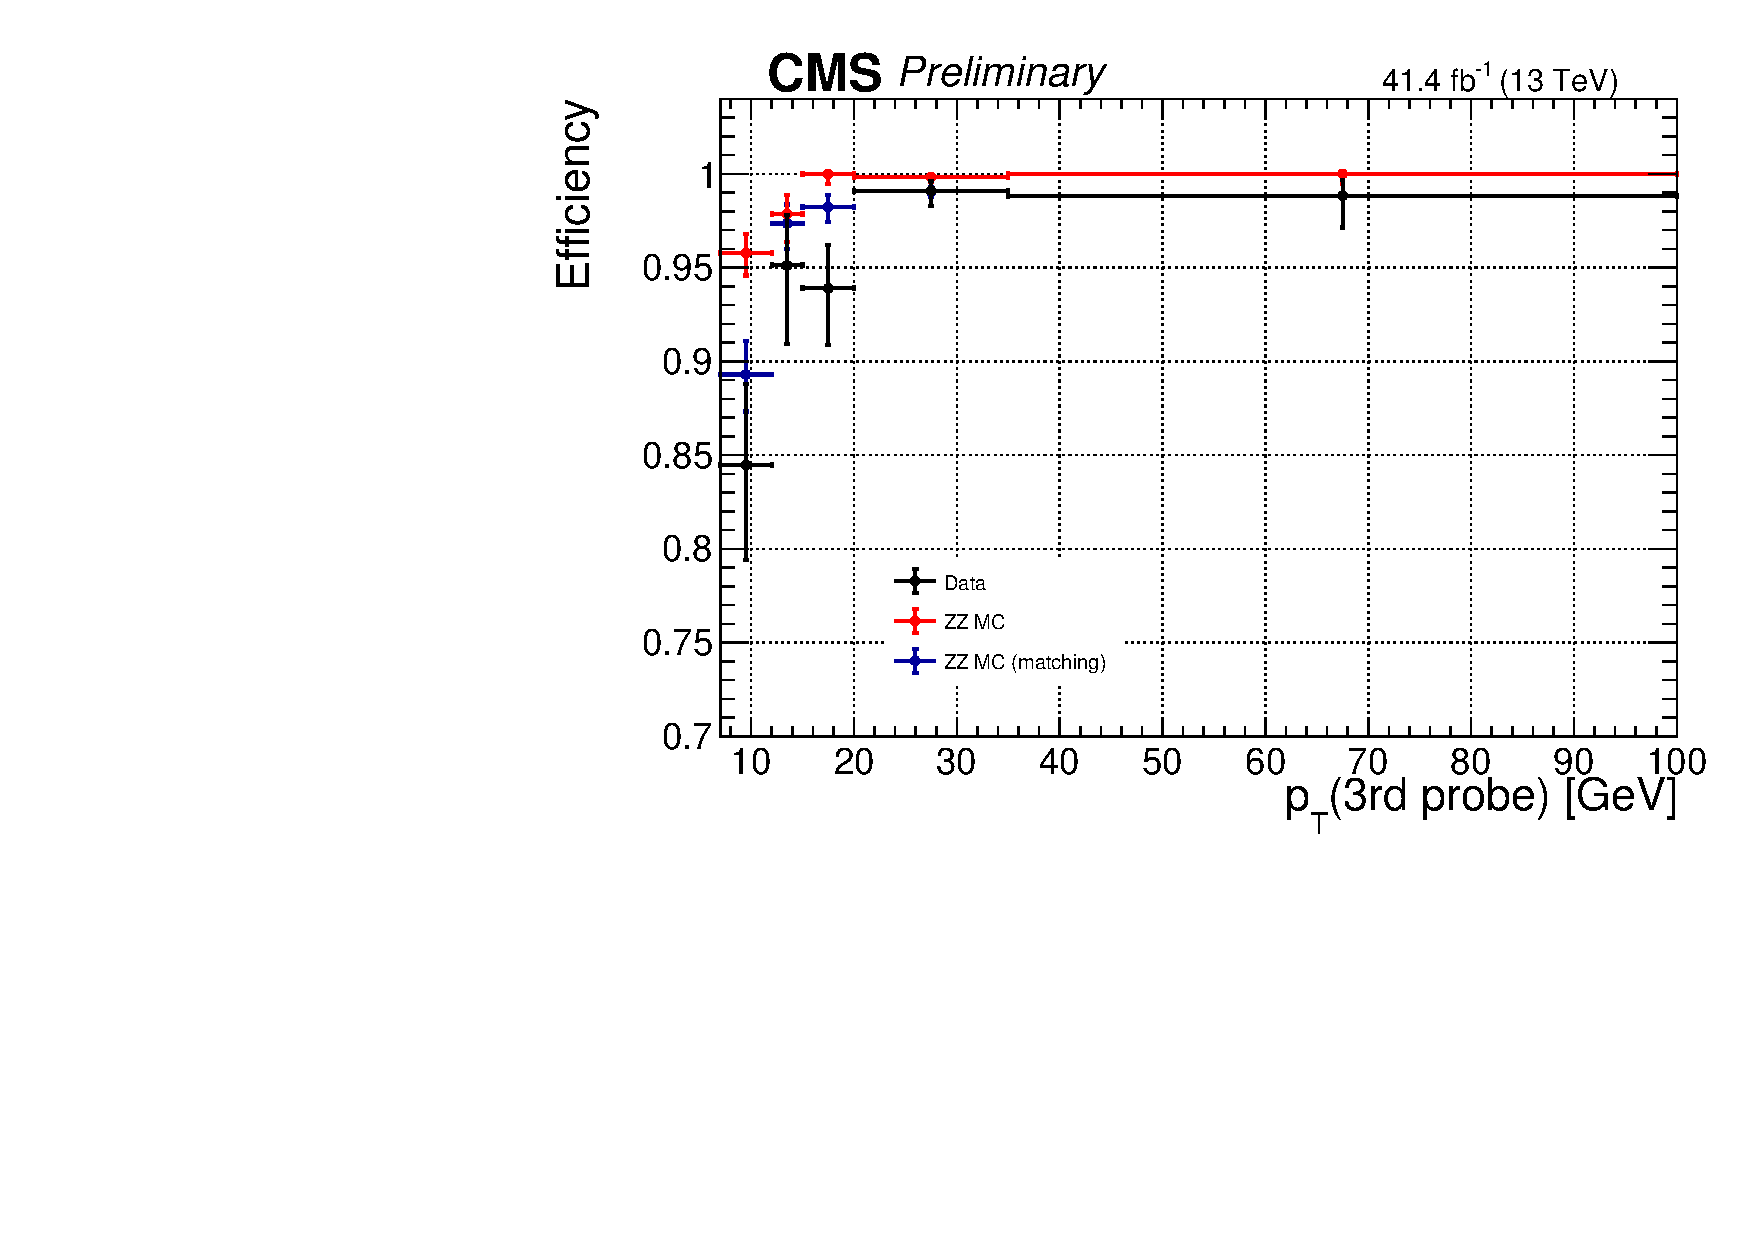
\includegraphics[width=0.45\textwidth]{Figures/Trigger17/Histo_TrigEff_ptMin_4e_mZ2_12.pdf} 
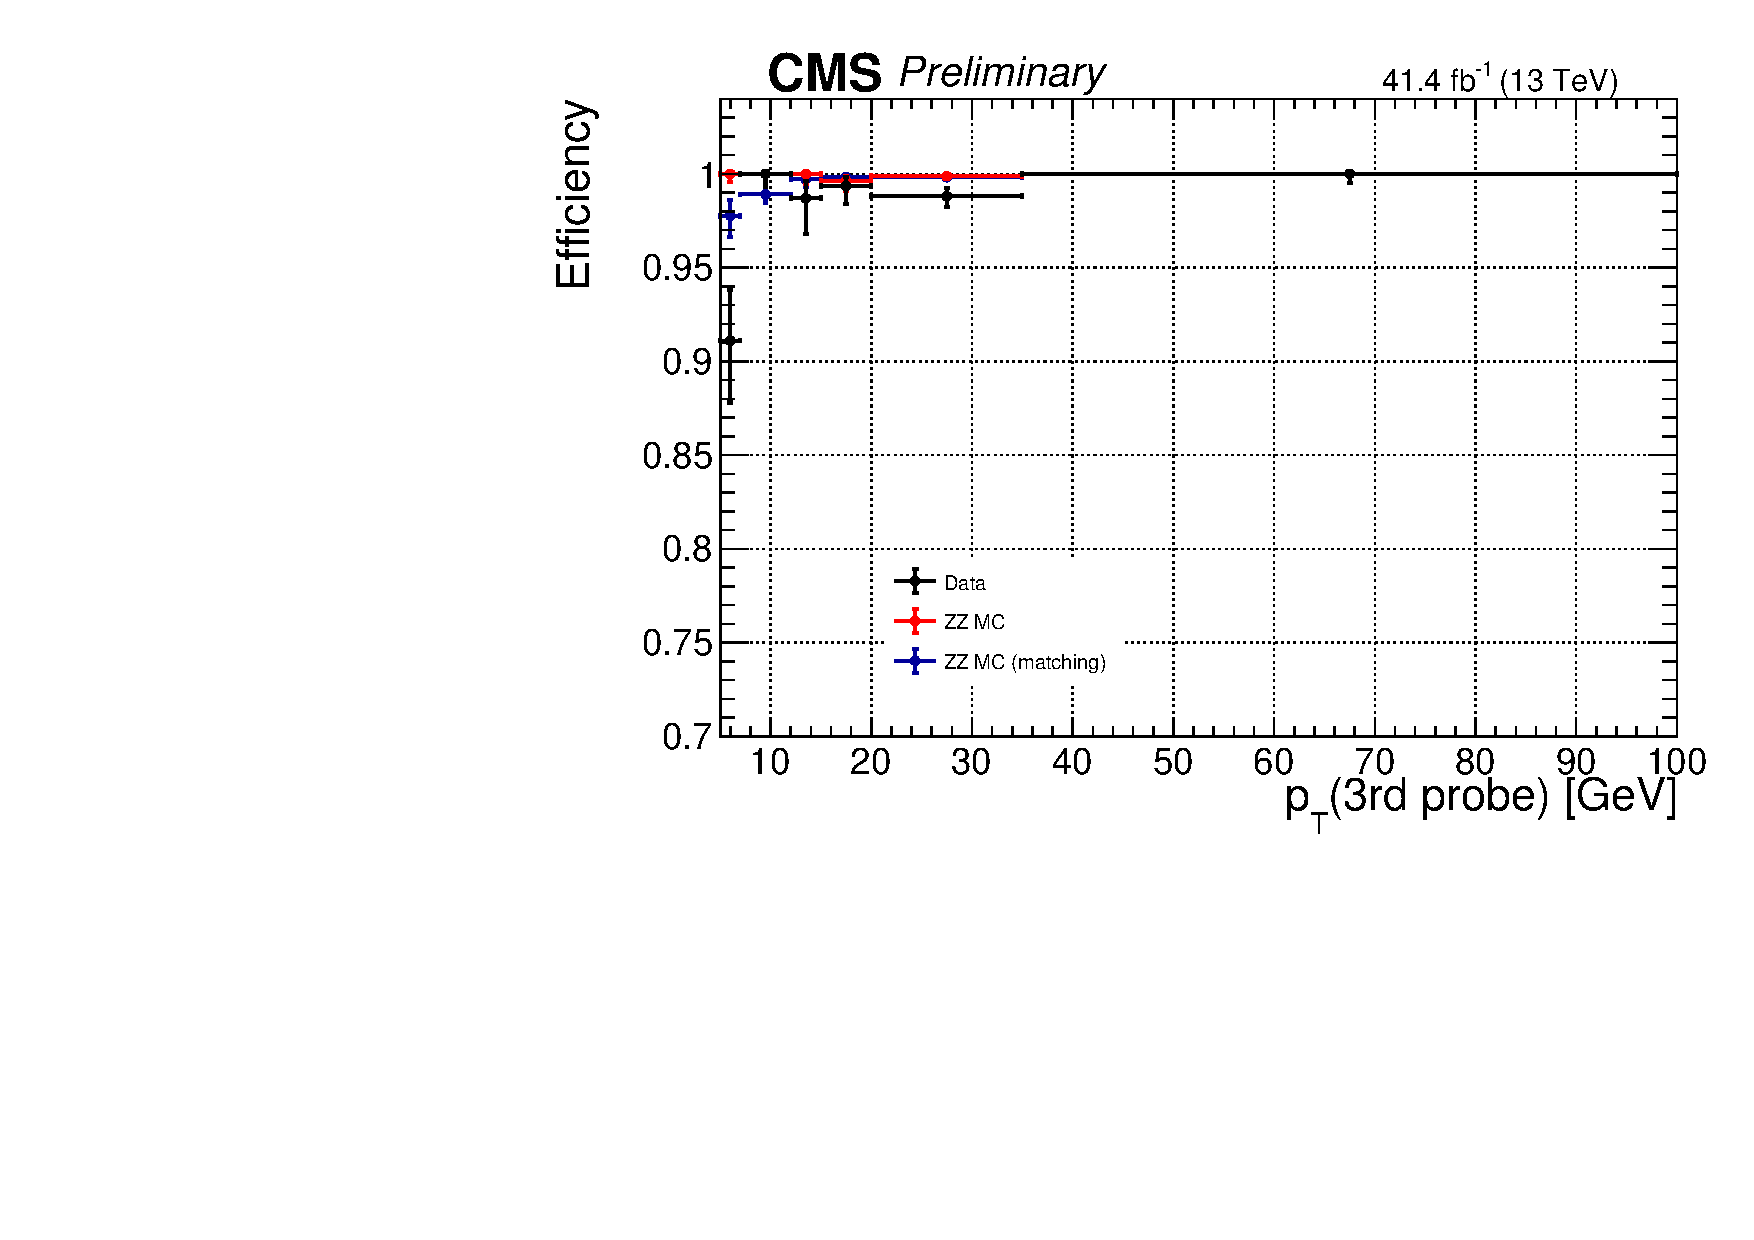
\includegraphics[width=0.45\textwidth]{Figures/Trigger17/Histo_TrigEff_ptMin_4mu_mZ2_12.pdf} \\
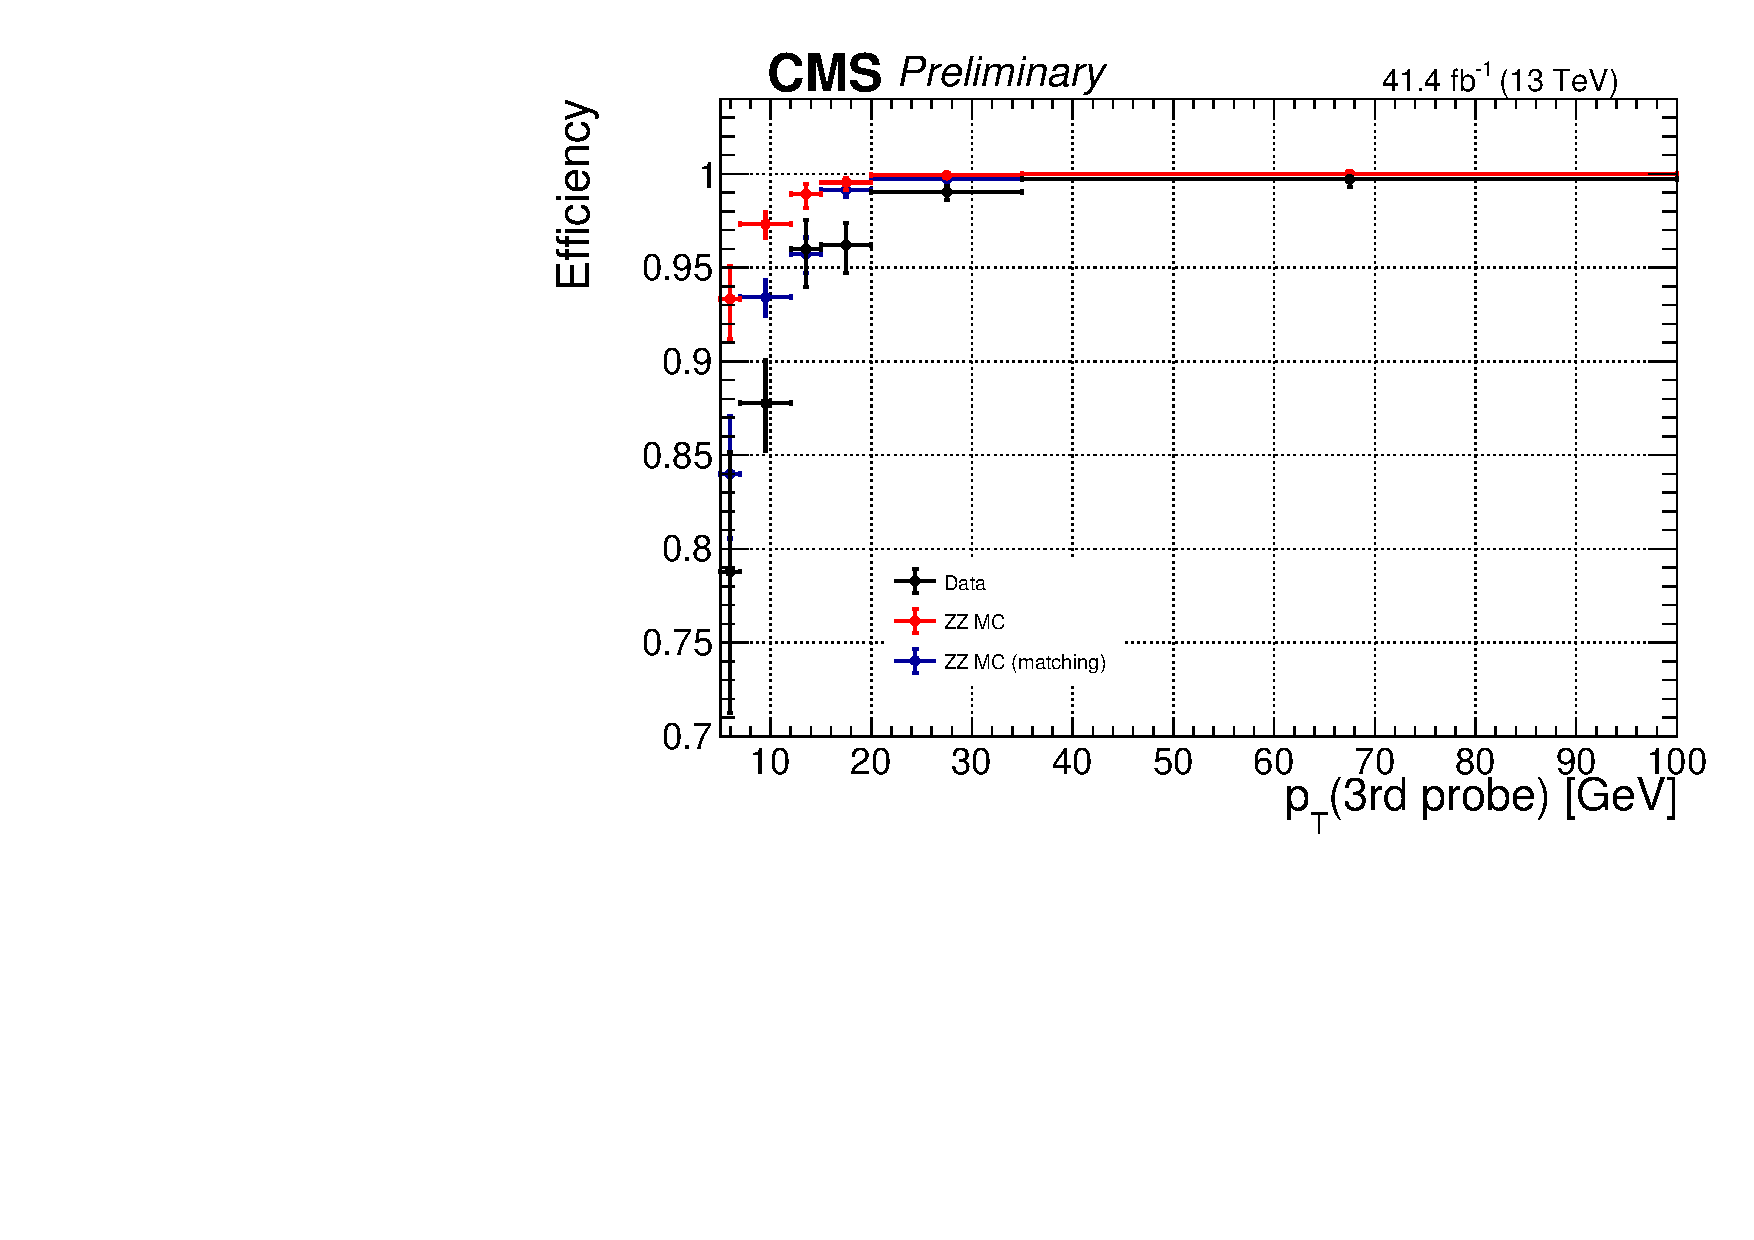
\includegraphics[width=0.45\textwidth]{Figures/Trigger17/Histo_TrigEff_ptMin_2e2mu_mZ2_12.pdf} 
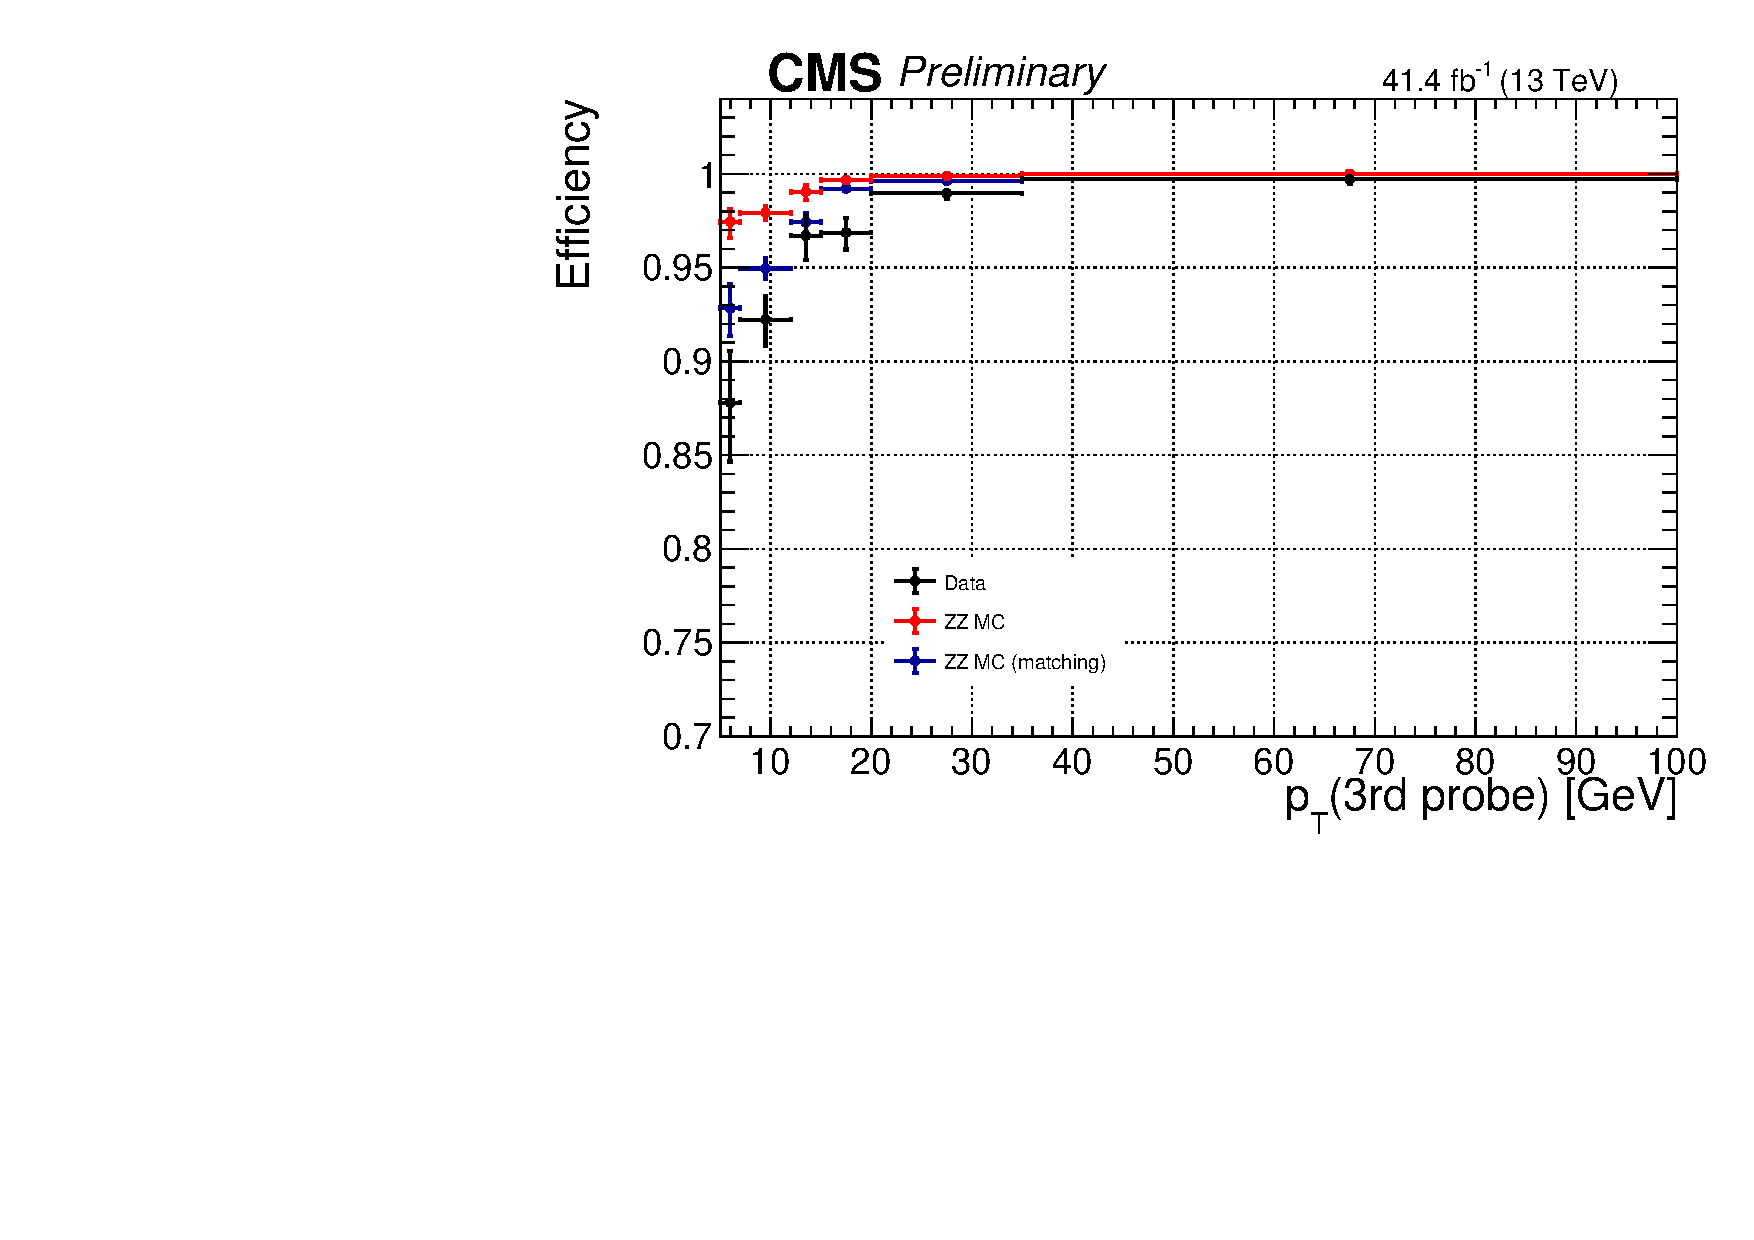
\includegraphics[width=0.45\textwidth]{Figures/Trigger17/Histo_TrigEff_ptMin_4l_mZ2_12.pdf} \\
\caption{[Placeholder for 2018] Trigger efficiency measured in data with Run 2018 using $4\ell$ events collected by 
    single lepton triggers for the $4e$ (top left), $4\mu$ (top right), $2e2\mu$ (bottom left) and $4\ell$ (bottom right) final states. 
%\fixme{Results using Prompt Reco, to be redone with ReReco}.
\label{fig:TrigEff_18}}
\end{center}
\end{figure}

\subsection{Simulation}

\subsubsection{Signal Samples}
Signal samples are generated by using LO {\sc Madgraph}, with the Hidden Abelian Higgs Model (HAHM)~\cite{Curtin:2014cca}.
Signal events are generated with  the physics process $p p \rightarrow H \rightarrow Z \zd \rightarrow 4\ell$, where 
$\ell = e, \mu$, with the kinematic parameter fixed to $\epsilon = 0.02$ and \mass{\zd} to be $4~\GeV$, $7~\GeV$,  
$10~\GeV$, $15~\GeV$, $20~\GeV$, $25~\GeV$, $30~\GeV$, $35~\GeV$. Kinematic distributions of the Madgraph samples 
are compared to the state-of-the-art {\sc powheg V2}~\cite{Alioli:2008gx,Nason:2004rx,Frixione:2007vw}+{\sc JHUgen} 
generator~\cite{Gao:2010qx}, and event kinematics are found to be similar, as shown in Section~\ref{sec:app-01-sigmc}.
Cross sections for each \zd signal are calculated by using multiplying the $N^3LO$ Higgs production cross section~\cite{Anastasiou:2016cez} 
with the branching fraction of $H \rightarrow Z \zd \rightarrow 4\ell$. Figure~\ref{fig:BrZd} shows branching fractions 
$Br(\zd \rightarrow \ell\ell)$ and $Br(H \rightarrow Z \zd \rightarrow 4\ell)$.

\begin{figure}[!htb]
\vspace*{0.3cm}
\begin{center}
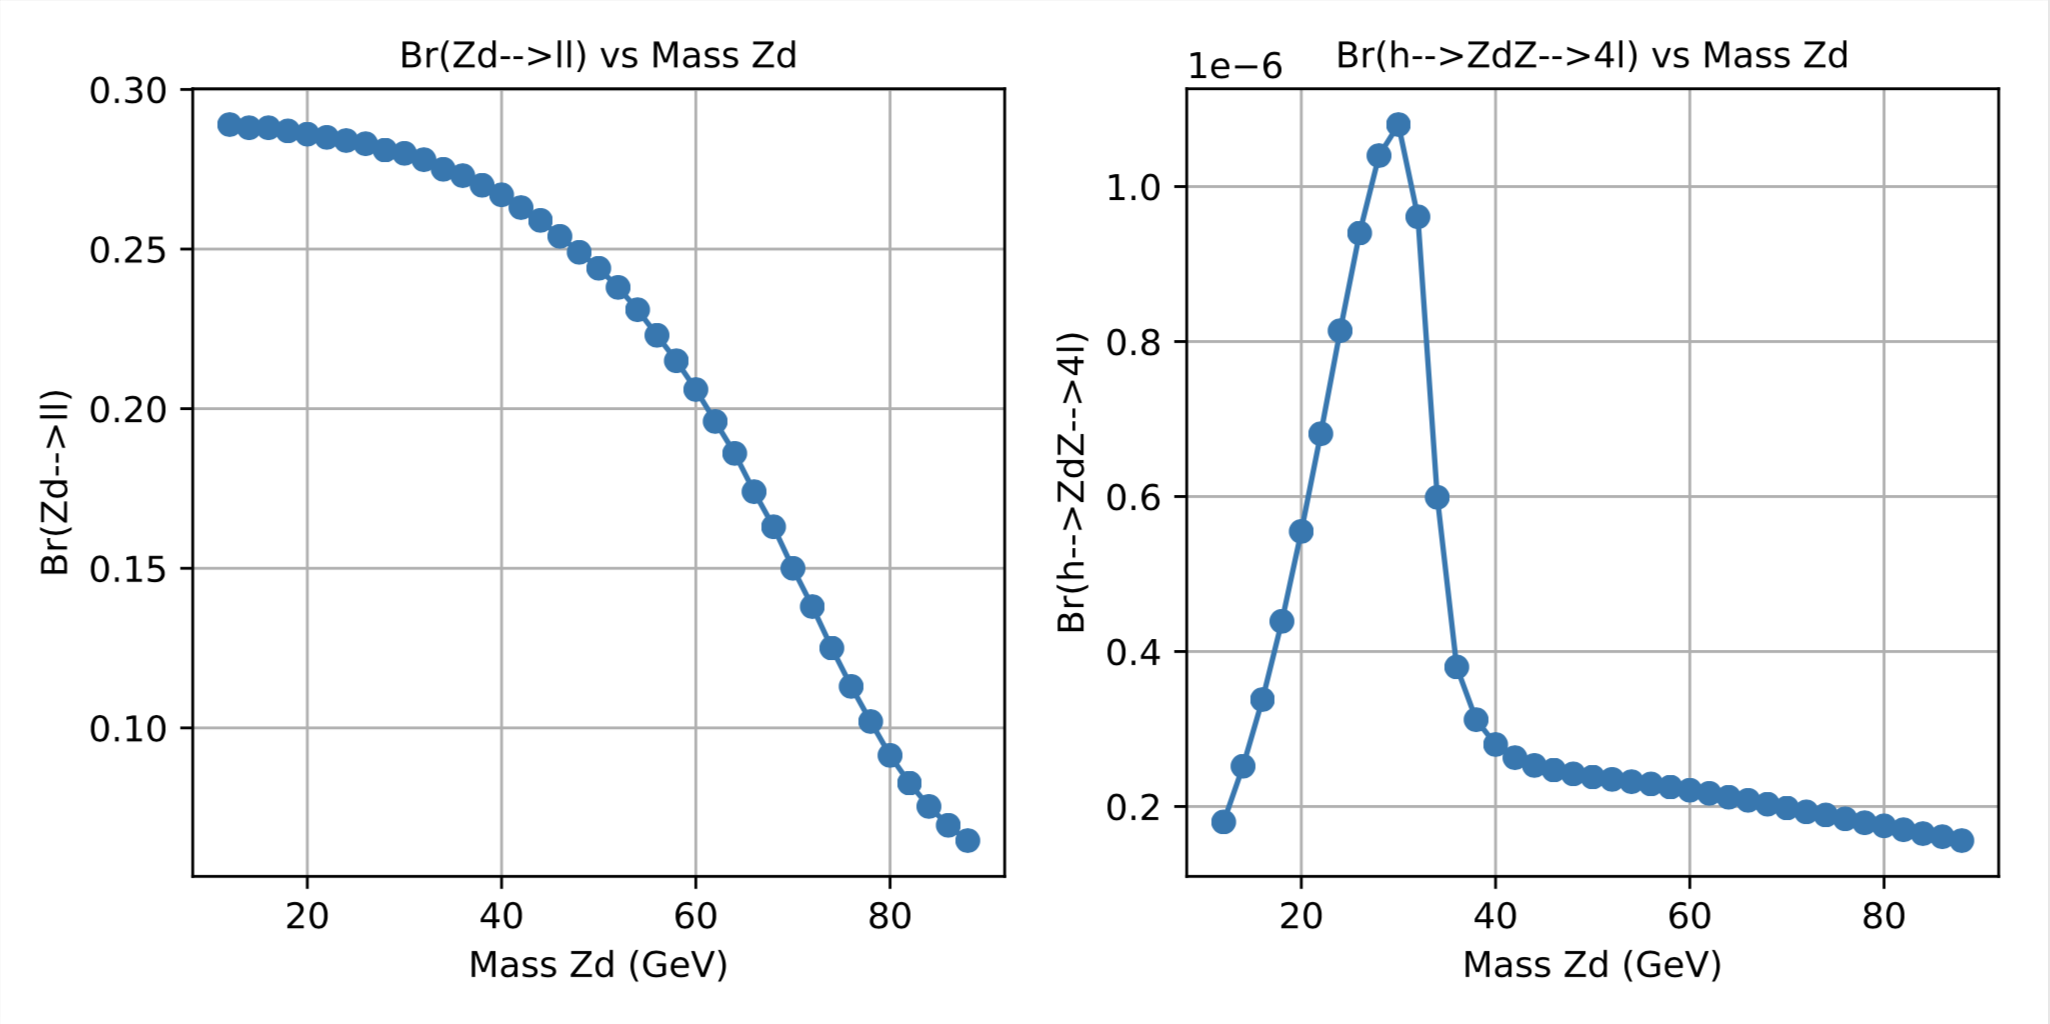
\includegraphics[width=1.0\textwidth]{Figures/Model/BrZd.png} 
\caption{Branching fraction $Br(\zd \rightarrow \ell\ell)$ (left) and $Br(H \rightarrow Z \zd \rightarrow 4\ell)$ (right)~\cite{Curtin:2014cca}.
\label{fig:BrZd}}
\end{center}
\end{figure}

\subsubsection{Background Samples}
Descriptions of the SM Higgs boson production are obtained using the 
{\sc powheg V2} generator for the five main production modes: 
gluon fusion ($\ggH$) including quark mass effects~\cite{Bagnaschi:2011tu}, vector boson fusion 
(VBF)~\cite{Nason:2009ai}, and associated production (WH, $\cPZ$H and \ttbar$\,$H~\cite{Hartanto:2015uka}). 
In the case of WH and $\cPZ$H the {\sc MiNLO HVJ} extension of {\sc powheg} is used~\cite{Luisoni:2013kna}. 
The description of the decay of the Higgs boson to four leptons is obtained using the {\sc JHUgen} 
generator. In the case of WH, $\cPZ$H and \ttbar$\,$H, the Higgs boson is allowed
to decay to H$\to \cPZ \cPZ \to 2\ell2$X such that 4-lepton events where two leptons originate from 
the decay of associated $\cPZ$, W bosons or top quarks are also taken into account in the simulation. 
Showering of parton-level events is done using {\sc pythia8.209}, and in all cases matching is performed by 
allowing QCD emissions at all energies in the shower and vetoing them afterwards according to the 
{\sc powheg} internal scale. All samples are generated with the NNPDF 3.0 NLO parton distribution 
functions (PDFs)~\cite{Ball:2014uwa}. The list of SM Higgs boson samples and their cross sections are shown in 
Table~\ref{tab:HiggsSamples_16}-\ref{tab:HiggsSamples_18}.

\begin{table}
\begin{scriptsize}
    \centering
    \begin{tabular}{|l|l|r|}
   \hline
 Process & Dataset Name & $\sigma\times BR (\times\epsilon_{\text{filter}})$ \\ \hline
 $\rm{gg}\to\rm{H}\to\cPZ\cPZ \to 4\ell$ & /GluGluHToZZTo4L\_M125\_13TeV\_powheg2\_JHUgenV6\_pythia8/[1] & $12.18~\rm{fb}$ \\ % & $12.12~\rm{fb}$ \\
 $\rm{qq}\to\rm{Hqq}\to\cPZ\cPZ\rm{qq}\to4\ell qq$ & /VBF\_HToZZTo4L\_M125\_13TeV\_powheg2\_JHUgenV6\_pythia8/[1] & $1.044~\rm{fb}$ \\ % $1.034~\rm{fb}$ \\
 $\rm{q\bar{q}}\to\rm{W^{+}H}\to\rm{W^{+}}\cPZ\cPZ\to4\ell+\rm{X}$ & /WplusH\_HToZZTo4L\_M125\_13TeV\_powheg2-minlo-HWJ\_JHUgenV6\_pythia8/[1] & $0.232~\rm{fb}$ \\ % $0.2339~\rm{fb}$ \\
 $\rm{q\bar{q}}\to\rm{W^{-}H}\to\rm{W^{-}}\cPZ\cPZ\to4\ell+\rm{X}$ & /WminusH\_HToZZTo4L\_M125\_13TeV\_powheg2-minlo-HWJ\_JHUgenV6\_pythia8/[1] & $0.147~\rm{fb}$ \\ % $0.1471~\rm{fb}$ \\
 $\rm{q\bar{q}}\to\cPZ \rm{H}\to\cPZ\cPZ\cPZ\to4\ell+\rm{X}$ & /ZH\_HToZZ\_4LFilter\_M125\_13TeV\_powheg2-minlo-HZJ\_JHUgenV6\_pythia8/[1] & $0.668~\rm{fb}$ \\ % $0.652~\rm{fb}$ \\
 $\rm{gg}\to\rm{ttH} \to\rm{tt}\cPZ\cPZ\to4\ell+\rm{X}$ & /ttH\_HToZZ\_4LFilter\_M125\_13TeV\_powheg\_JHUgen\_pythia8/[1] & $0.393~\rm{fb}$ \\ % $0.337~\rm{fb}$ \\ 
 \hline
 \multicolumn{3}{l}{[1] RunIISummer16MiniAODv2-PUMoriond17\_80X\_mcRun2\_asymptotic\_2016\_TrancheIV\_v6-v1} \\
 \end{tabular}
 \caption{SM Higgs boson Monte Carlo samples and cross sections in 2016.}
  \label{tab:HiggsSamples_16}
\end{scriptsize}
\end{table}

\begin{table}
\begin{scriptsize}
    \centering
    \begin{tabular}{|l|l|r|}
   \hline
 Process & Dataset Name & $\sigma\times BR (\times\epsilon_{\text{filter}})$ \\ \hline
 $\rm{gg}\to\rm{H}\to\cPZ\cPZ \to 4\ell$ & /GluGluHToZZTo4L\_M125\_13TeV\_powheg2\_JHUgenV6\_pythia8/[1] & $12.18~\rm{fb}$ \\ % & $12.12~\rm{fb}$ \\
 $\rm{qq}\to\rm{Hqq}\to\cPZ\cPZ\rm{qq}\to4\ell qq$ & /VBF\_HToZZTo4L\_M125\_13TeV\_powheg2\_JHUgenV6\_pythia8/[1] & $1.044~\rm{fb}$ \\ % $1.034~\rm{fb}$ \\
 $\rm{q\bar{q}}\to\rm{W^{+}H}\to\rm{W^{+}}\cPZ\cPZ\to4\ell+\rm{X}$ & /WplusH\_HToZZTo4L\_M125\_13TeV\_powheg2-minlo-HWJ\_JHUgenV6\_pythia8/[1] & $0.232~\rm{fb}$ \\ % $0.2339~\rm{fb}$ \\
 $\rm{q\bar{q}}\to\rm{W^{-}H}\to\rm{W^{-}}\cPZ\cPZ\to4\ell+\rm{X}$ & /WminusH\_HToZZTo4L\_M125\_13TeV\_powheg2-minlo-HWJ\_JHUgenV6\_pythia8/[1] & $0.147~\rm{fb}$ \\ % $0.1471~\rm{fb}$ \\
 $\rm{q\bar{q}}\to\cPZ \rm{H}\to\cPZ\cPZ\cPZ\to4\ell+\rm{X}$ & /ZH\_HToZZ\_4LFilter\_M125\_13TeV\_powheg2-minlo-HZJ\_JHUgenV6\_pythia8/[1] & $0.668~\rm{fb}$ \\ % $0.652~\rm{fb}$ \\
 $\rm{gg}\to\rm{ttH} \to\rm{tt}\cPZ\cPZ\to4\ell+\rm{X}$ & /ttH\_HToZZ\_4LFilter\_M125\_13TeV\_powheg\_JHUgen\_pythia8/[1] & $0.393~\rm{fb}$ \\ % $0.337~\rm{fb}$ \\ 
 \hline
 \multicolumn{3}{l}{[1] RunIISummer16MiniAODv2-PUMoriond17\_80X\_mcRun2\_asymptotic\_2016\_TrancheIV\_v6-v1} \\
 \end{tabular}
 \caption{[Placeholder for 2017] SM Higgs boson Monte Carlo samples and cross sections in 2017.}
  \label{tab:HiggsSamples_17}
\end{scriptsize}
\end{table}

\begin{table}
\begin{scriptsize}
    \centering
    \begin{tabular}{|l|l|r|}
   \hline
 Process & Dataset Name & $\sigma\times BR (\times\epsilon_{\text{filter}})$ \\ \hline
 $\rm{gg}\to\rm{H}\to\cPZ\cPZ \to 4\ell$ & /GluGluHToZZTo4L\_M125\_13TeV\_powheg2\_JHUgenV6\_pythia8/[1] & $12.18~\rm{fb}$ \\ % & $12.12~\rm{fb}$ \\
 $\rm{qq}\to\rm{Hqq}\to\cPZ\cPZ\rm{qq}\to4\ell qq$ & /VBF\_HToZZTo4L\_M125\_13TeV\_powheg2\_JHUgenV6\_pythia8/[1] & $1.044~\rm{fb}$ \\ % $1.034~\rm{fb}$ \\
 $\rm{q\bar{q}}\to\rm{W^{+}H}\to\rm{W^{+}}\cPZ\cPZ\to4\ell+\rm{X}$ & /WplusH\_HToZZTo4L\_M125\_13TeV\_powheg2-minlo-HWJ\_JHUgenV6\_pythia8/[1] & $0.232~\rm{fb}$ \\ % $0.2339~\rm{fb}$ \\
 $\rm{q\bar{q}}\to\rm{W^{-}H}\to\rm{W^{-}}\cPZ\cPZ\to4\ell+\rm{X}$ & /WminusH\_HToZZTo4L\_M125\_13TeV\_powheg2-minlo-HWJ\_JHUgenV6\_pythia8/[1] & $0.147~\rm{fb}$ \\ % $0.1471~\rm{fb}$ \\
 $\rm{q\bar{q}}\to\cPZ \rm{H}\to\cPZ\cPZ\cPZ\to4\ell+\rm{X}$ & /ZH\_HToZZ\_4LFilter\_M125\_13TeV\_powheg2-minlo-HZJ\_JHUgenV6\_pythia8/[1] & $0.668~\rm{fb}$ \\ % $0.652~\rm{fb}$ \\
 $\rm{gg}\to\rm{ttH} \to\rm{tt}\cPZ\cPZ\to4\ell+\rm{X}$ & /ttH\_HToZZ\_4LFilter\_M125\_13TeV\_powheg\_JHUgen\_pythia8/[1] & $0.393~\rm{fb}$ \\ % $0.337~\rm{fb}$ \\ 
 \hline
 \multicolumn{3}{l}{[1] RunIISummer16MiniAODv2-PUMoriond17\_80X\_mcRun2\_asymptotic\_2016\_TrancheIV\_v6-v1} \\
 \end{tabular}
 \caption{SM Higgs boson Monte Carlo samples and cross sections in 2018.}
  \label{tab:HiggsSamples_18}
\end{scriptsize}
\end{table}



Production of $ZZ$ via quark-antiquark annihilation is generated at
next-to-leading order (NLO) using {\sc powheg V2}~\cite{Nason:2013ydw}
and {\sc pythia8}, with 
the same settings as for the Higgs signal. As this simulation covers a large
range of ZZ invariant masses, dynamical QCD factorization and renormalization
scales have been chosen, equal to $m_{\cPZ\cPZ}$. 

The $\Pg\Pg \! \to \! ZZ$ process is simulated at leading order (LO) 
with MCFM~\cite{MCFM,Campbell:2013una}. In order to match the 
$\Pg\Pg \! \to \mathrm{H} \to \! ZZ$ transverse momentum spectra predicted 
by {\sc powheg} at NLO, the showering for MCFM samples is performed with 
different {\sc pythia8} settings, allowing only emissions up to the parton-level scale
(``wimpy'' shower).

Although not directly used to model data observations, additional 
MC samples of W$\cPZ$, Drell-Yan+jets, \ttbar, and tribosons are
generated using {\sc MadGraph5\_aMCatNLO}~\cite{Alwall:2014hca} either
inclusively or merging several jet multiplicities, as detailed in the table.
Table~\ref{tab:MCSamples_16}-\ref{tab:MCSamples_18} summarizes background MC samples used for this analysis. 


\begin{table}
\begin{footnotesize}
    \centering
    \begin{tabular}{|l|l|r|}
   \hline
 Process & Dataset Name & $\sigma\cdot BR$ \\ \hline
 $\rm{qq} \to \cPZ\cPZ \to 4\ell$ & /ZZTo4L\_13TeV\_powheg\_pythia8/[1] & $1.256 \rm{pb}$ \\
 $\rm{qq} \to \cPZ\cPZ \to 4\ell$ & /ZZTo4L\_13TeV-amcatnloFXFX-pythia8/[1] & $1.212 \rm{pb}$ \\
 $\rm{gg} \rightarrow \cPZ\cPZ \to 4e$ & /GluGluToContinToZZTo4e\_13TeV\_MCFM701/[1] & $0.00159 \rm{ pb}$ \\
 $\rm{gg} \rightarrow \cPZ\cPZ \to 4$$\mu$ & /GluGluToContinToZZTo4mu\_13TeV\_MCFM701/[1] & $0.00159 \rm{ pb}$ \\
 $\rm{gg} \rightarrow \cPZ\cPZ \to 4$$\tau$ & /GluGluToContinToZZTo4tau\_13TeV\_MCFM701/[1] & $0.00159 \rm{ pb}$ \\
 $\rm{gg} \rightarrow \cPZ\cPZ \to 2e2$$\mu$ & /GluGluToContinToZZTo2e2mu\_13TeV\_MCFM701/[1] & $0.00319 \rm{ pb}$ \\
 $\rm{gg} \rightarrow \cPZ\cPZ \to 2e2$$\tau$ & /GluGluToContinToZZTo2e2tau\_13TeV\_MCFM701/[1] & $0.00319 \rm{ pb}$ \\
 $\rm{gg} \rightarrow \cPZ\cPZ \to 2$$\mu2$$\tau$ & /GluGluToContinToZZTo2mu2tau\_13TeV\_MCFM701/[1] & $0.00319 \rm{ pb}$ \\ \hline
 $\cPZ \to \ell\ell$ + jets & /DYJetsToLL\_M-50\_TuneCUETP8M1\_13TeV-amcatnloFXFX-pythia8/[1] & $6104 \rm{ pb}$ \\
 $\cPZ \to \ell\ell$ + jets  & /DYJetsToLL\_M-10to50\_TuneCUETP8M1\_13TeV-amcatnloFXFX-pythia8/[1] & $18610 \rm{ pb}$ \\ \hline
 %W$\cPZ \to 3\ell\nu$ & /WZJets\_TuneCUETP8M1\_13TeV-amcatnloFXFX-pythia8/[1] &  $5.29 \rm{pb}$ \\ 
 W$\cPZ \to 3\ell\nu$ & /WZTo3LNu\_TuneCUETP8M1\_13TeV-powheg-pythia8/[1] & $4.430 \rm{ pb}$ \\ \hline
 $t\bar{t}$ & /TTJets\_TuneCUETP8M1\_13TeV-amcatnloFXFX-pythia8/[1] & $815.96 \rm{ pb}$ \\ 
 $t\bar{t} \to 2\ell2\nu 2b$ & /TTTo2L2Nu\_13TeV-powheg/[1] &  $87.31 \rm{pb}$ \\ \hline
% WWZ & /WWZ\_TuneCUETP8M1\_13TeV-amcatnlo-pythia8/[2] & $0.1651 \rm{ pb}$ \\
% W\cPZ\cPZ & /WZZ\_TuneCUETP8M1\_13TeV-amcatnlo-pythia8/[2] & $0.05565 \rm{ pb}$ \\
% \cPZ\cPZ\cPZ & /ZZZ\_TuneCUETP8M1\_13TeV-amcatnlo-pythia8/[2] & $0.01398 \rm{ pb}$ \\ \hline
 \multicolumn{3}{l}{[1] RunIISummer16MiniAODv2-PUMoriond17\_80X\_mcRun2\_asymptotic\_2016\_TrancheIV\_v6-v1} \\
 \end{tabular}
 \caption{Background Monte Carlo samples and cross sections for Run 2016.}
  \label{tab:MCsamples_16}
\end{footnotesize}
\end{table}

\begin{table}
\begin{footnotesize}
\centering
\begin{tabular}{|l|l|r|}
\hline
 Process & Dataset Name & $\sigma\cdot BR$ \\ \hline
 $\rm{qq} \to \cPZ\cPZ \to 4\ell$ & /ZZTo4L\_13TeV\_powheg\_pythia8/[1] & $1.256 \rm{pb}$ \\
 $\rm{qq} \to \cPZ\cPZ \to 4\ell$ & /ZZTo4L\_13TeV-amcatnloFXFX-pythia8/[1] & $1.212 \rm{pb}$ \\
 $\rm{gg} \rightarrow \cPZ\cPZ \to 4e$ & /GluGluToContinToZZTo4e\_13TeV\_MCFM701/[1] & $0.00159 \rm{ pb}$ \\
 $\rm{gg} \rightarrow \cPZ\cPZ \to 4$$\mu$ & /GluGluToContinToZZTo4mu\_13TeV\_MCFM701/[1] & $0.00159 \rm{ pb}$ \\
 $\rm{gg} \rightarrow \cPZ\cPZ \to 4$$\tau$ & /GluGluToContinToZZTo4tau\_13TeV\_MCFM701/[1] & $0.00159 \rm{ pb}$ \\
 $\rm{gg} \rightarrow \cPZ\cPZ \to 2e2$$\mu$ & /GluGluToContinToZZTo2e2mu\_13TeV\_MCFM701/[1] & $0.00319 \rm{ pb}$ \\
 $\rm{gg} \rightarrow \cPZ\cPZ \to 2e2$$\tau$ & /GluGluToContinToZZTo2e2tau\_13TeV\_MCFM701/[1] & $0.00319 \rm{ pb}$ \\
 $\rm{gg} \rightarrow \cPZ\cPZ \to 2$$\mu2$$\tau$ & /GluGluToContinToZZTo2mu2tau\_13TeV\_MCFM701/[1] & $0.00319 \rm{ pb}$ \\ \hline
 $\cPZ \to \ell\ell$ + jets & /DYJetsToLL\_M-50\_TuneCUETP8M1\_13TeV-amcatnloFXFX-pythia8/[1] & $6104 \rm{ pb}$ \\
 $\cPZ \to \ell\ell$ + jets  & /DYJetsToLL\_M-10to50\_TuneCUETP8M1\_13TeV-amcatnloFXFX-pythia8/[1] & $18610 \rm{ pb}$ \\ \hline
 %W$\cPZ \to 3\ell\nu$ & /WZJets\_TuneCUETP8M1\_13TeV-amcatnloFXFX-pythia8/[1] &  $5.29 \rm{pb}$ \\ 
 W$\cPZ \to 3\ell\nu$ & /WZTo3LNu\_TuneCUETP8M1\_13TeV-powheg-pythia8/[1] & $4.430 \rm{ pb}$ \\ \hline
 $t\bar{t}$ & /TTJets\_TuneCUETP8M1\_13TeV-amcatnloFXFX-pythia8/[1] & $815.96 \rm{ pb}$ \\ 
 $t\bar{t} \to 2\ell2\nu 2b$ & /TTTo2L2Nu\_13TeV-powheg/[1] &  $87.31 \rm{pb}$ \\ \hline
% WWZ & /WWZ\_TuneCUETP8M1\_13TeV-amcatnlo-pythia8/[2] & $0.1651 \rm{ pb}$ \\
% W\cPZ\cPZ & /WZZ\_TuneCUETP8M1\_13TeV-amcatnlo-pythia8/[2] & $0.05565 \rm{ pb}$ \\
% \cPZ\cPZ\cPZ & /ZZZ\_TuneCUETP8M1\_13TeV-amcatnlo-pythia8/[2] & $0.01398 \rm{ pb}$ \\ \hline
% \multicolumn{3}{l}{[1] RunIISummer16MiniAODv2-PUMoriond17\_80X\_mcRun2\_asymptotic\_2016\_TrancheIV\_v6-v1} \\
\multicolumn{3}{l}{[1] RunIIFall17MiniAOD-94X\_mc2017\_realistic\_v10\_v1}\\
 \end{tabular}
 \caption{Background Monte Carlo samples and cross sections for Run 2017.}
  \label{tab:MCsamples_17}
\end{footnotesize}
\end{table}

\begin{table}
\begin{footnotesize}
    \centering
    \begin{tabular}{|l|l|r|}
   \hline
 Process & Dataset Name & $\sigma\cdot BR$ \\ \hline
 $\rm{qq} \to \cPZ\cPZ \to 4\ell$ & /ZZTo4L\_13TeV\_powheg\_pythia8/[1] & $1.256 \rm{pb}$ \\
 $\rm{qq} \to \cPZ\cPZ \to 4\ell$ & /ZZTo4L\_13TeV-amcatnloFXFX-pythia8/[1] & $1.212 \rm{pb}$ \\
 $\rm{gg} \rightarrow \cPZ\cPZ \to 4e$ & /GluGluToContinToZZTo4e\_13TeV\_MCFM701/[1] & $0.00159 \rm{ pb}$ \\
 $\rm{gg} \rightarrow \cPZ\cPZ \to 4$$\mu$ & /GluGluToContinToZZTo4mu\_13TeV\_MCFM701/[1] & $0.00159 \rm{ pb}$ \\
 $\rm{gg} \rightarrow \cPZ\cPZ \to 4$$\tau$ & /GluGluToContinToZZTo4tau\_13TeV\_MCFM701/[1] & $0.00159 \rm{ pb}$ \\
 $\rm{gg} \rightarrow \cPZ\cPZ \to 2e2$$\mu$ & /GluGluToContinToZZTo2e2mu\_13TeV\_MCFM701/[1] & $0.00319 \rm{ pb}$ \\
 $\rm{gg} \rightarrow \cPZ\cPZ \to 2e2$$\tau$ & /GluGluToContinToZZTo2e2tau\_13TeV\_MCFM701/[1] & $0.00319 \rm{ pb}$ \\
 $\rm{gg} \rightarrow \cPZ\cPZ \to 2$$\mu2$$\tau$ & /GluGluToContinToZZTo2mu2tau\_13TeV\_MCFM701/[1] & $0.00319 \rm{ pb}$ \\ \hline
 $\cPZ \to \ell\ell$ + jets & /DYJetsToLL\_M-50\_TuneCUETP8M1\_13TeV-amcatnloFXFX-pythia8/[1] & $6104 \rm{ pb}$ \\
 $\cPZ \to \ell\ell$ + jets  & /DYJetsToLL\_M-10to50\_TuneCUETP8M1\_13TeV-amcatnloFXFX-pythia8/[1] & $18610 \rm{ pb}$ \\ \hline
 %W$\cPZ \to 3\ell\nu$ & /WZJets\_TuneCUETP8M1\_13TeV-amcatnloFXFX-pythia8/[1] &  $5.29 \rm{pb}$ \\ 
 W$\cPZ \to 3\ell\nu$ & /WZTo3LNu\_TuneCUETP8M1\_13TeV-powheg-pythia8/[1] & $4.430 \rm{ pb}$ \\ \hline
 $t\bar{t}$ & /TTJets\_TuneCUETP8M1\_13TeV-amcatnloFXFX-pythia8/[1] & $815.96 \rm{ pb}$ \\ 
 $t\bar{t} \to 2\ell2\nu 2b$ & /TTTo2L2Nu\_13TeV-powheg/[1] &  $87.31 \rm{pb}$ \\ \hline
% WWZ & /WWZ\_TuneCUETP8M1\_13TeV-amcatnlo-pythia8/[2] & $0.1651 \rm{ pb}$ \\
% W\cPZ\cPZ & /WZZ\_TuneCUETP8M1\_13TeV-amcatnlo-pythia8/[2] & $0.05565 \rm{ pb}$ \\
% \cPZ\cPZ\cPZ & /ZZZ\_TuneCUETP8M1\_13TeV-amcatnlo-pythia8/[2] & $0.01398 \rm{ pb}$ \\ \hline
 \multicolumn{3}{l}{[1] RunIISummer16MiniAODv2-PUMoriond17\_80X\_mcRun2\_asymptotic\_2016\_TrancheIV\_v6-v1} \\
 \end{tabular}
 \caption{[Placeholder for 2018] Background Monte Carlo samples and cross sections.}
  \label{tab:MCsamples_18}
\end{footnotesize}
\end{table}




\section{Objects}
\label{sec:obj}

This analysis follows the same object definition as in~\cite{AN-16-442,AN-17-342}, and are 
described as follows.

\subsection{Electrons}

\subsubsection{Electron Reconstruction}
\label{sec:eleReco}
More details on electron reconstruction can be found in Ref.~\cite{ElectronLegacy}. 

Electron candidates are preselected using loose cuts on track-cluster matching observables, so as to preserve the highest possible efficiency while rejecting part of the QCD background. To be considered for the analysis, electrons are required to have a
transverse momentum $p^e_T >$ 7 GeV, a reconstructed $|\eta^e| <$ 2.5, and to satisfy a loose primary vertex 
constraint defined as $d_{xy} < 0.5$ and $d_z < 1$. 
Such electrons are called {\bf loose electrons}.

The early runs in the 2016 data-taking exhibit an tracking inefficiency originating from a reduced hit reconstruction efficiency in the strip detector (``HIP" effect). 
The resulting data-MC discrepancy is corrected using scale factors as is done for the electron selection with data efficiencies measured using the same tag-and-probe technique outlined later (see Section~\ref{sec:eleEffMeas}). 
These studies are carried out by the EGM POG and the results are only summarised here.

The electron reconstruction scale factors are shown Fig.~\ref{fig:ele_rec_scale_factors} as a one-dimensional function of the super cluster $\eta$ only, as it was shown that the \pt dependence of the scale factor is negligible.

\begin{figure}[!htb]
\vspace*{0.3cm}
\begin{center}
\includegraphics[width=0.6\textwidth]{Figures/Electrons/ele_rec_scale_factors.pdf}
\end{center}
\caption{Electron reconstruction efficiencies efficiency in data versus $\eta$ and data/MC scale factors as provided by the EGM POG.}
\label{fig:ele_rec_scale_factors}
\end{figure}


\subsubsection{Electron Identification}
\label{sec:eleID}
Reconstructed electrons are identified by means of a Gradient Boosted Decision Tree (GBDT) multivariate classifier algorithm, which exploits observables from the electromagnetic cluster, the matching between the cluster and the electron track as well as observables based exclusively on tracking measurements. 
The BDT has been retrained using CMSSW\_8\_0\_X samples.

The classifier is trained on  Drell-Yan plus jets MC sample for both signal and background: 
{
\tiny  
\begin{verbatim}
/DYJetsToLL_M-50_TuneCUETP8M1_13TeV-madgraphMLM-pythia8/RunIISpring16DR80-PUSpring16_80X_mcRun2_asymptotic_2016_v3_ext1-v1/
\end{verbatim}
}

The impact of the retraining of the ID for the 2016 conditions is illustrated in the ROC curves shown in Fig.~\ref{fig:ele_ID_ROC}. Several studies to improve the performance of the MVA for the harsher 2016 running conditions were performed. 
One study considered a new spitting of the BDT training bins, where electrons falling into the gap regions of the ECAL, e.g. the EB-EE transition region, where trained separately from the non-gap electrons. 
No improvement for either population is observed, indicating that the current setup is already able to properly take the significantly differing input distributions in those regions into account. 
Also studied where additional variables including more cluster-shape observables. 
None of these variables helped to improve the performance in the relevant $>95\%$ signal efficiency regime, though up to $20\%$ improved background rejection was seen for $80\%$ working points. 
Finally, the hyper-parameters of the MVA were systematically scanned for their optimal values. The resulting configuration was found to improve the overall performance only marginally by $<10\%$, however, introducing a significant overtraining effect. 
Due to the small gains and large overtraining, it was decided to not modify the hyper-parameters beyond the interface changes coming from changing to the latest 4.2.0 version of the TMVA package.

Figure~\ref{fig:ele_ID_BDT_output} shows the output of the BDT on the training and testing samples for true and fake electrons 
for the high-$p_T$ training bin in the endcap. 
The good agreement between the training and testing distributions is similar across the 6 training bins and indicates that the classifier has not been overtrained.

\begin{figure}[!htb]
\vspace*{0.3cm}
\begin{center}
\includegraphics[width=0.80\textwidth]{Figures/Electrons/ele_ROC.png}
\caption{Performance comparison of the MVA trained for the 2015 analysis and the retraining for 2016 conditions. 
The respective working points are indicated by the markers.
\label{fig:ele_ID_ROC}}
\end{center}
\end{figure}

\begin{figure}[!htb]
\vspace*{0.3cm}
\begin{center}
\includegraphics[width=0.5\textwidth]{Figures/Electrons/ele_overtraining.png}
\caption{BDT output for the training and testing sample for true and fake electrons in the high-$p_T$ endcap training bins.
\label{fig:ele_ID_BDT_output}}
\end{center}
\end{figure}

Table~\ref{tab:ele_ID_input_variables_16}-\ref{tab:ele_ID_input_variables_18} summarizes the full list of observables used as input to the classifier
and table~\ref{tab:ele_ID_WP_16}-\ref{tab:ele_ID_WP_18} lists the cut values applied to the BDT score for the chosen working point. 
For the analysis, we define {\bf tight electrons} as the loose electrons that pass this MVA identification working point. 

 \begin{table}[h!]
\scriptsize
    \centering
    \begin{tabular}{c|l}
\hline %----------------------------------------------------------------------------------------
\hline %----------------------------------------------------------------------------------------
%\multicolumn{4}{|c|}{Datasets}                                                                \\
observable type    &  observable name      	\\
\hline %----------------------------------------------------------------------------------------

\multirow{6}{*}{cluster shape}
	&  RMS of the energy-crystal number spectrum along $\eta$ and $\varphi$; $\sigma_{i\eta i\eta}$, $\sigma_{i\varphi i\varphi}$		\\
	&  super cluster width along $\eta$ and $\phi$		\\
	&  'ratio of the hadronic energy behind the electron 
supercluster to the supercluster energy, $H/E$			\\
	&  circularity $(E_{5\times5} - E_{5\times1})/E_{5\times5}$			\\
	&  sum of the seed and adjacent crystal over the super cluster energy $R_{9}$			\\
	&  for endcap traing bins: energy fraction in pre-shower $E_{PS}/E_{raw}$			\\
\hline
\multirow{2}{*}{track-cluster matching}
	& energy-momentum agreement $E_{tot}/p_{in}$, $E_{ele}/p_{out}$, $1/E_{tot} - 1/p_{in}$ 			\\
	& position matching $\Delta\eta_{in}$, $\Delta\varphi_{in}$, $\Delta\eta_{seed}$			\\
\hline
\multirow{5}{*}{tracking}
        & fractional momentum loss $f_{brem} = 1 - p_{out}/p_{in}$	\\
        & number of hits of the KF and GSF track $N_{KF}$, $N_{GSF}$ $(\mathord{\cdot})$ \\
        & reduced $\chi^2$ of the KF and GSF track $\chi^{2}_{KF}$, $\chi^{2}_{\textrm{GSF}}$ \\
        & number of expected but missing inner hits $(\mathord{\cdot})$ 	\\
        & probability transform of conversion vertex fit $\chi^2$ $(\mathord{\cdot})$ \\

\hline %----------------------------------------------------------------------------------------
\hline %----------------------------------------------------------------------------------------
     \end{tabular}
\small
    \caption{Overview of input variables to the identification classifier in Run 2016. Variables not used in the run I MVA are marked with  $(\mathord{\cdot})$.}
    \label{tab:ele_ID_input_variables_16}
\end{table}

 \begin{table}[h!]
\scriptsize
    \centering
    \begin{tabular}{c|l}
\hline %----------------------------------------------------------------------------------------
\hline %----------------------------------------------------------------------------------------
%\multicolumn{4}{|c|}{Datasets}                                                                \\
observable type    &  observable name      	\\
\hline %----------------------------------------------------------------------------------------

\multirow{6}{*}{cluster shape}
	&  RMS of the energy-crystal number spectrum along $\eta$ and $\varphi$; $\sigma_{i\eta i\eta}$, $\sigma_{i\varphi i\varphi}$		\\
	&  super cluster width along $\eta$ and $\phi$		\\
	&  'ratio of the hadronic energy behind the electron 
supercluster to the supercluster energy, $H/E$			\\
	&  circularity $(E_{5\times5} - E_{5\times1})/E_{5\times5}$			\\
	&  sum of the seed and adjacent crystal over the super cluster energy $R_{9}$			\\
	&  for endcap traing bins: energy fraction in pre-shower $E_{PS}/E_{raw}$			\\
\hline
\multirow{2}{*}{track-cluster matching}
	& energy-momentum agreement $E_{tot}/p_{in}$, $E_{ele}/p_{out}$, $1/E_{tot} - 1/p_{in}$ 			\\
	& position matching $\Delta\eta_{in}$, $\Delta\varphi_{in}$, $\Delta\eta_{seed}$			\\
\hline
\multirow{5}{*}{tracking}
        & fractional momentum loss $f_{brem} = 1 - p_{out}/p_{in}$	\\
        & number of hits of the KF and GSF track $N_{KF}$, $N_{GSF}$ $(\mathord{\cdot})$ \\
        & reduced $\chi^2$ of the KF and GSF track $\chi^{2}_{KF}$, $\chi^{2}_{\textrm{GSF}}$ \\
        & number of expected but missing inner hits $(\mathord{\cdot})$ 	\\
        & probability transform of conversion vertex fit $\chi^2$ $(\mathord{\cdot})$ \\
\hline
\multirow{3}{*}{isolation}
& Particle Flow photon isolation sum $(\mathord{\cdot})$ \\
& Particle Flow charged hadrons isolation sum $(\mathord{\cdot})$ \\
& Particle Flow neutral hadrons isolation sum $(\mathord{\cdot})$ \\
\hline
\multirow{1}{*}{For PU-resilience}
& Mean energy density in the event: $\rho$ $(\mathord{\cdot})$ \\
\hline %----------------------------------------------------------------------------------------
\hline %----------------------------------------------------------------------------------------
     \end{tabular}
\small
    \caption{Overview of input variables to the identification classifier in Run 2017. Variables not used in the run I MVA are marked with  $(\mathord{\cdot})$.}
    \label{tab:ele_ID_input_variables_17}
\end{table}

 \begin{table}[h!]
\scriptsize
    \centering
    \begin{tabular}{c|l}
\hline %----------------------------------------------------------------------------------------
\hline %----------------------------------------------------------------------------------------
%\multicolumn{4}{|c|}{Datasets}                                                                \\
observable type    &  observable name      	\\
\hline %----------------------------------------------------------------------------------------

\multirow{6}{*}{cluster shape}
	&  RMS of the energy-crystal number spectrum along $\eta$ and $\varphi$; $\sigma_{i\eta i\eta}$, $\sigma_{i\varphi i\varphi}$		\\
	&  super cluster width along $\eta$ and $\phi$		\\
	&  'ratio of the hadronic energy behind the electron 
supercluster to the supercluster energy, $H/E$			\\
	&  circularity $(E_{5\times5} - E_{5\times1})/E_{5\times5}$			\\
	&  sum of the seed and adjacent crystal over the super cluster energy $R_{9}$			\\
	&  for endcap traing bins: energy fraction in pre-shower $E_{PS}/E_{raw}$			\\
\hline
\multirow{2}{*}{track-cluster matching}
	& energy-momentum agreement $E_{tot}/p_{in}$, $E_{ele}/p_{out}$, $1/E_{tot} - 1/p_{in}$ 			\\
	& position matching $\Delta\eta_{in}$, $\Delta\varphi_{in}$, $\Delta\eta_{seed}$			\\
\hline
\multirow{5}{*}{tracking}
        & fractional momentum loss $f_{brem} = 1 - p_{out}/p_{in}$	\\
        & number of hits of the KF and GSF track $N_{KF}$, $N_{GSF}$ $(\mathord{\cdot})$ \\
        & reduced $\chi^2$ of the KF and GSF track $\chi^{2}_{KF}$, $\chi^{2}_{\textrm{GSF}}$ \\
        & number of expected but missing inner hits $(\mathord{\cdot})$ 	\\
        & probability transform of conversion vertex fit $\chi^2$ $(\mathord{\cdot})$ \\

\hline %----------------------------------------------------------------------------------------
\hline %----------------------------------------------------------------------------------------
     \end{tabular}
\small
\caption{[Placeholder for 2018] Overview of input variables to the identification classifier in Run 2018. Variables not used in the run I MVA are marked with  $(\mathord{\cdot})$.}
    \label{tab:ele_ID_input_variables_18}
\end{table}


\begin{table}[h!]
\scriptsize
    \centering
    \begin{tabular}{c|c c c}
%\multicolumn{4}{|c|}{Datasets}                                                                \\
\hline %----------------------------------------------------------------------------------------
minimum BDT score    &  $|\eta| < 0.8 $ & $0.8 < |\eta| < 1.479$ 	& $|\eta| > 1.479$      \\
\hline %----------------------------------------------------------------------------------------
$ 5 < p_T < 10 $ GeV &  -0.211      & -0.396  		& -0.215		\\
$p_T > 10$ GeV       &  -0.870		& -0.838		& -0.763		\\
\hline %----------------------------------------------------------------------------------------
\hline %----------------------------------------------------------------------------------------
     \end{tabular}
\small
    \caption{Minimum BDT score required for passing the electron identification in Run 2016.}
    \label{tab:ele_ID_WP_16}
\end{table}

\begin{table}[h!]
\scriptsize
    \centering
    \begin{tabular}{c|c c c}
%\multicolumn{4}{|c|}{Datasets}                                                                \\
\hline %----------------------------------------------------------------------------------------
minimum BDT score    &  $|\eta| < 0.8 $ & $0.8 < |\eta| < 1.479$ 	& $|\eta| > 1.479$      \\
\hline %----------------------------------------------------------------------------------------
$ 5 < p_T < 10 $ GeV &  0.628      & 0.592  		& 0.637		\\
$p_T > 10$ GeV       &  0.036		& 0.043		& -0.266		\\
\hline %----------------------------------------------------------------------------------------
\hline %----------------------------------------------------------------------------------------
     \end{tabular}
\small
    \caption{Minimum BDT score required for passing the electron identification in Run 2017.}% \textbf{FIXME: WP to be defined!}}
    \label{tab:ele_ID_WP}
\end{table}

\begin{table}[h!]
\scriptsize
    \centering
    \begin{tabular}{c|c c c}
%\multicolumn{4}{|c|}{Datasets}                                                                \\
\hline %----------------------------------------------------------------------------------------
minimum BDT score    &  $|\eta| < 0.8 $ & $0.8 < |\eta| < 1.479$ 	& $|\eta| > 1.479$      \\
\hline %----------------------------------------------------------------------------------------
$ 5 < p_T < 10 $ GeV &  -0.211      & -0.396  		& -0.215		\\
$p_T > 10$ GeV       &  -0.870		& -0.838		& -0.763		\\
\hline %----------------------------------------------------------------------------------------
\hline %----------------------------------------------------------------------------------------
     \end{tabular}
\small
\caption{[Placeholder for 2018] Minimum BDT score required for passing the electron identification in Run 2018.}
    \label{tab:ele_ID_WP_18}
\end{table}


% Finally, the measurement of the signal efficiencies in data and the data-MC scale factors are presented in section~\ref{sec:eleEffMeas}. 



\subsubsection{Electron Isolation}
\label{sec:eleiso}
The relative isolation for electrons is then defined as: 

\begin{equation}
\text{RelPFiso} = (\sum_{\text{charged}} p_T + \sum^{\text{corr}}_{\text{neutral}} p_T)/p_T^{\text{lepton}}  .
\label{eqn:elepfrelisoeqn}
\end{equation} 

where the corrected neutral component of isolation is then computed using the formula :

\begin{equation}
\label{eqn:neutralea}
  \sum^{\text{corr}}_{\text{neutral}} p_T = \text{max}(\sum^{\text{uncorr}}_{\text{neutral}} p_T - \rho \times A_\text{eff},0 \GeV)  .
\end{equation}

and the mean pile-up contribution to the isolation cone is obtained as :  
\begin{equation}
 PU =  \rho \times A_\text{eff}
\label{eqn:purho}
\end{equation}

where $\rho$ is the mean energy density in the event and the effective area $A_{eff}$ is defined as the ratio
between the slope of the average isolation and that of $\rho$ as a function of the number of vertices. 

The electron isolation working point was optimized in Ref.~\cite{AN-15-277} and the electron isolation working was 
chosen to be $\text{RelPFiso}(\Delta R = 0.3) < 0.35$. 


\subsubsection{Electron Energy Calibrations}
Electrons in data are corrected for features in ECAL energy scale
in bins of $\pt$ and $\left| \eta \right|$. Corrections are calculated
on a $\cPZ \to \Pe\Pe$ sample to align the dielectron 
mass spectrum in the data to that in the MC, and to
minimize its width.

The $\cPZ \to \Pe\Pe$ mass resolution in Monte Carlo is made to match
data by applying a pseudorandom Gaussian smearing to electron energies,
with Gaussian parameters varying in bins of $\pt$ and $\left| \eta \right|$.
This has the effect of convoluting the electron energy spectrum with a
Gaussian.



The electron energy scale is measured in data by fitting a Crystall-ball function to the di-electron mass spectrum around the Z peak in the $Z+\ell$ control region. 
The energy scale for the full 2016 dataset is shown in Fig.~\ref{fig:ele_energy_scale}(a) and agrees with the MC with 100~MeV. 
The stability of the energy scale across different run periods is shown in Fig.~\ref{fig:ele_energy_scale}(b), where the data is binned into approximately 500~pb luminosity blocks.

\begin{figure}[!htb]
\vspace*{0.3cm}
\begin{center}
\subfigure [] {\resizebox{7.5cm}{!}{\includegraphics{Figures/Electrons/ele_energy_scale.pdf}}}
\subfigure [] {\resizebox{9.5cm}{!}{\includegraphics{Figures/Electrons/ele_energy_scale_per_lumi.pdf}}}
\end{center}
\caption{
(a): electron energy scale measured in the $Z+\ell$ control region for EB and EE electrons. The results of the Crystall-ball fit are reported in the figure. 
(b): lepton energy scales per 500~pb luminosity block. 

}
\label{fig:ele_energy_scale}
\end{figure}


%\begin{figure}[!htb]
%\vspace*{0.3cm}
%\begin{center}
%\includegraphics[width=0.7\textwidth]{Figures/Electrons/ele_energy_scale}
%\end{center}
%\caption{Electron energy scale measured in the $Z+\ell$ control region. The results of the Crystall-bal fit are reported in the figure.}
%\label{fig:ele_energy_scale}
%\end{figure}
%
%\begin{figure}[!htb]
%\vspace*{0.3cm}
%\begin{center}
%\includegraphics[width=0.8\textwidth]{Figures/Electrons/ele_energy_scale_per_lumi}
%\end{center}
%\caption{Lepton energy scales per 500~pb luminosity block. Note: discrepancy in run G was fixed (bug in calibration application); need to update plot.}
%\label{fig:ele_energy_scale_per_lumi}
%\end{figure}

%The effect of these corrections on a single-$\cPZ$ sample is shown in
%Fig.~\ref{fig:ZeeCorrections} for, from left to right, with both electrons in the barrel,
%one electron in the endcap and one in the barrel, and both electrons in the endcap. The top
%row shows the fit to the data and MC distributions before the correction, and the bottom
%row shows the fits after the correction.

%\begin{figure}[htbp]
%  \begin{center}
%    \subfigure[]{\includegraphics[width=0.32\textwidth]{Figures/Zee-BB_comp_before.pdf}}
%    \subfigure[]{\includegraphics[width=0.32\textwidth]{Figures/Zee-BE_comp_before.pdf}}
%    \subfigure[]{\includegraphics[width=0.32\textwidth]{Figures/Zee-EE_comp_before.pdf}} \\
%    \subfigure[]{\includegraphics[width=0.32\textwidth]{Figures/Zee-BB_comp_after.pdf}}
%    \subfigure[]{\includegraphics[width=0.32\textwidth]{Figures/Zee-BE_comp_after.pdf}}
%    \subfigure[]{\includegraphics[width=0.32\textwidth]{Figures/Zee-EE_comp_after.pdf}} \\
%    \caption{
%      Effect of electron energy corrections and smearing for single-$\cPZ$
%      events with both electrons in the barrel (left), one electron in the
%      barrel and one in the endcaps (middle), and both electrons in the
%      endcaps (right). Plots in the top row are uncorrected, and plots in the
%      bottom row have the corrections and smearing applied.
%    }
%    \label{fig:ZeeCorrections}
%  \end{center}
%\end{figure}


\subsubsection{Electron Efficiency Measurements}
\label{sec:eleEffMeas}
The Tag-and-Probe study was performed on the single electron primary datasets listed in table \ref{tab:datasets_data} using the same golden JSON of 36.8 
fb$^{-1}$ as for the main analysis. More details on the Tag-and-Probe method can be found in Ref.~\cite{AN-15-277}. 

Tag electrons need to satisfy the following quality requirements:
\begin{itemize}
\item trigger matched to HLT\_Ele27\_eta2p1\_WPTight\_Gsf\_v*
\item $p_{T} > 30$~GeV, super cluster (SC) $\eta < 2.1$ but on in EB-EE gap ($1.4442<|\eta|<1.566$)
\item tight working point of the Spring16 cut-based electron ID
\end{itemize}

Probe electrons only need to be reconstructed as GsfElectron. The FSR recovery algorithm used in the main analysis is used consistently throughout the efficiency measurement: the isolations are calculated without any FSR photons matched to electrons and the probe electron \pt as well as the di-electron invariant mass include the FSR photons, if any. 


The nominal MC efficiencies are evaluated from the LO MadGraph Drell-Yan sample, while the NLO systematics use the 0,1 jet MadGraph\_AMCatNLO sample listed in Table \ref{tab:MCsamples}.

In contrast to previous efficiency measurements, a template fit is used here. The $m_{ee}$ signal shape of the passing and failing probes is taken from MC and convoluted with a Gaussian. The data is then fitted with the convoluted MC template and a CMSShape (an Error-function with a one-sided exponential tail). This change follows from the usage of the new T\&P tool developed by the EGM POG.


%\paragraph{Electron selection efficiency measurements}\mbox{}\\
%\label{par:Efficiency_measurements}

The electron selection efficiency is measured as a function of the probe electron $p_{T}$ and its SC $\eta$, and separately for electrons falling in the ECAL gaps. Figure \ref{fig:ele_sel_pt_turn_on} shows the $\p_{T}$ turn-on curves measured in data, and the final 2D scale factor is shown in Fig.~\ref{fig:ele_sel_scale_factors} together with the systematic uncertainties. These scale factors are very similar to the ICHEP figures, but more homogenous across $\eta$ and $p_{T}$ because of the higher statistics and the usage of more stable fitting routines in the new T\&P tool.


\begin{figure}[!htb]
\begin{center}
    \subfigure [] {\resizebox{7.5cm}{!}{\includegraphics{Figures/Electrons/ele_eff_pt.pdf}}}
    \subfigure [] {\resizebox{7.5cm}{!}{\includegraphics{Figures/Electrons/gap_ele_eff_pt.pdf}}}\\
\caption{Electron selection efficiencies measured using the Tag-and-Probe technique described in the text, non-gap electrons (left) and gap electrons (right).}
\label{fig:ele_sel_pt_turn_on}
\end{center}
\end{figure}

\begin{figure}[!htb]
\begin{center}
    \subfigure [] {\resizebox{15cm}{!}{\includegraphics{Figures/Electrons/ele_eff_sf_unc.pdf}}}\\
    \subfigure [] {\resizebox{15cm}{!}{\includegraphics{Figures/Electrons/gap_ele_eff_sf_unc.pdf}}}
\caption{Electron selection efficiencies measured using the Tag-and-Probe technique described in the text, non-gap electrons (top) and gap electrons (bottom).}
\label{fig:ele_sel_scale_factors}
\end{center}
\end{figure}


%\paragraph{Systematic uncertainties}\mbox{}\\
%\label{par:Systematic_uncertainties}
%%%%%%%%%%%%%%%%%%%%%%%%%%%%

 The EGM recommendations on the evaluation of Tag-and-Probe uncertainties for efficiency measurements are followed. Specifically, we consider

\begin{itemize}
   \item Variation of the signal shape from a MC shape to an analytic shape (Crystal Ball) fitted to the MC
   \item Variation of the background shape from a CMS-shape to a simple exponential in fits to data
   \item Variation of the tag selection: tag $p_{T}>$35~GeV and passes MVA-based 8X ID
   \item Using an NLO MC sample for the signal templates
\end{itemize}

The total uncertainty for the measurement of the scale factors is the quadratic sum of the statistical uncertainties returned from the fit and the aforementioned systematic uncertainties.





\clearpage

\subsection{Muons}

\subsubsection{Muon Reconstruction and Identification}
\label{sec:muonReco}
More details on muon reconstruction can be found in Ref.~\cite{AN-15-277}.
We define {\bf loose muons} as the muons that satisfy  
$p_T > 5$, $|\eta| < 2.4$, $dxy< 0.5$, $dz < 1$, where $dxy$ and $dz$ are 
defined w.r.t. the PV and using the 'muonBestTrack'. Muons have to be 
reconstructed by either the Global Muon or Tracker Muon algorithm. Standalone 
Muon tracks that are only reconstructed in the muon system are rejected.
Muons with \verb|muonBestTrackType==2| (standalone) are discarded even if they 
are marked as global or tracker muons. 

Loose muons with $\pt$ below 200\GeV are considered {\bf tight muons} if they 
also pass the PF muon ID (note that the naming 
convention used for these IDs differs from the muon POG naming scheme, in which
the ``tight ID'' used here is called the ``loose ID''). Loose muons with $\pt$ 
above 200\GeV are considered tight muons if they pass the PF ID or the Tracker
High-$\pt$ ID, the definition of which is shown in Table~\ref{tab:highPtID}.
This relaxed definition is used to increase signal efficiency for the high-mass
search. When a very heavy resonance decays to two $\cPZ$ bosons, both bosons
will be very boosted. In the lab frame, the leptons coming from the decay of
a highly boosted $\cPZ$ will be nearly collinear, and the PF ID loses 
efficiency for muons separated by approximately $\Delta R < 0.4$, which roughly 
corresponds to muons originating from $\cPZ$ bosons with $\pt > 500\GeV$.

\begin{table}[h]
    \begin{small}
    \begin{center}
    \caption{
      The requirements for a muon to pass the Tracker High-$\pt$ ID. Note that
      these are equivalent to the Muon POG High-$\pt$ ID with the global track 
      requirements removed.
      }
    \begin{tabular}{|l|l|}
      \hline
      Plain-text description         & Technical description                 \\
      \hline
      Muon station matching          & Muon is matched to segments           \\
                                     & in at least two muon stations         \\
                                     & \textbf{NB: this implies the muon is} \\
                                     & \textbf{an arbitrated tracker muon.}  \\
      \hline                                                          
      Good $\pt$ measurement         & $\frac{\pt}{\sigma_{\pt}} < 0.3$      \\
      \hline
      Vertex compatibility ($x-y$)   & $d_{xy} < 2$~mm                       \\
      \hline
      Vertex compatibility ($z$)     & $d_{z} < 5$~mm                        \\
      \hline
      Pixel hits                     & At least one pixel hit                \\
      \hline
      Tracker hits                   & Hits in at least six tracker layers   \\
      \hline
    \end{tabular}
    \label{tab:highPtID}
    \end{center}
    \end{small}
\end{table}

An additional ``ghost-cleaning'' step is performed to deal with situations when a single muon
can be incorrectly reconstructed as two or more muons:

\begin{itemize}

\item Tracker Muons that are not Global Muons are required to be arbitrated.
\item If two muons are sharing 50\% or more of their segments then the muon with lower quality is removed.

\end{itemize}



\subsubsection{Muon Isolation}
\label{sec:muoniso}
Particle-Flow based isolation, described for electrons in section~\ref{sec:eleiso}, is also used for the muons. 
The only difference with electrons is the way the pileup contribution is subtracted: for the muons, $\Delta\beta$ correction is applied, whereby $\Delta\beta = \frac{1}{2} \sum^\text{charged had.}_\text{PU} \pt$  gives an estimate of the energy deposit of neutral particles (hadrons and photons) from pile-up vertices. 
The relative isolation for muons is then defined as:
\begin{equation}
\text{RelPFiso} = \frac{\sum^\text{charged had.} \pt + \max(\sum^\text{neutral had.} \ET 
+ \sum^\text{photon} \ET - \Delta \beta, 0)}{\pt^\text{lepton}}
\label{eqn:mupfiso}
\end{equation}

The isolation working point for muons was optimized in Ref.~\cite{AN-15-277} and the working point was chosen to be the same as electrons,
namely $\text{RelPFiso}(\Delta R = 0.3) < 0.35$. 



\subsubsection{Muon Energy Calibrations}
% \input{Objects/muCalib}


\subsubsection{Muon Efficiency Measurements}
\label{sec:muonEffMeas}
Muon efficiencies are measured with the Tag and Probe (T\&P) method performed on
$\cPZ \to \Pgm\Pgm$ and $\JPsi\to\mu\mu$ events in bins of $\pt$ and $\eta$. More
details on the methodology can be found in Ref.~\cite{AN-15-277}.
%
The $\Z$ sample is used to measure the muon reconstruction and identification efficiency at high $\pt$,
and the efficiency of the isolation and impact parameter requirements at all $\pt$.
%
The $\JPsi$ sample is used to measure the reconstruction efficiency at low $\pt$,
as it benefits from a better purity in that kinematic regime. In this case,
events are collected using \verb=HLT_Mu7p5_Track2_Jpsi_v*= when probing the
reconstruction and identification efficiency in the muon system, and using the
 \verb=HLT_Mu7p5_L2Mu2_Jpsi_v*= when probing the tracking efficiency.

\paragraph*{Reconstruction and identification}

Results for the muon reconstruction and identification efficiency for $\pt > 20\GeV$
have been derived by the Muon POG.
The probe in this measurement are tracks reconstructed in the inner tracker, and
the passing probes are those that are also reconstructed as a global or tracker muon 
and passing the Muon POG Loose muon identification.
%
Results for low \pt muons were derived using \JPsi events, with the same definitions
of probe and passing probes. The systematic uncertainties are estimated by varying the analytical signal and background shape models used to fit 
the dimuon invariant mass. Details on the procedure can be found in Ref.~\cite{AN-15-277}. The efficiency and scale 
factors used for low $\pt$ muons are the ones derived using single muon prompt-reco dataset.

The efficiency in data and simulation is shown in Fig.~\ref{fig:MuonIDEff_1}. 
\begin{figure}[htbp]
  \begin{center}
    \subfigure[]{\includegraphics[width=0.32\textwidth]{Figures/Muons/mu_Loose_barrel.pdf}}
    \subfigure[]{\includegraphics[width=0.32\textwidth]{Figures/Muons/mu_Loose_endcap.pdf}}
    \subfigure[]{\includegraphics[width=0.32\textwidth]{Figures/Muons/mu_Loose_pt7.pdf}}
    \caption{Muon reconstruction and identification efficiency at low \pt, measured with the tag\&probe method on \JPsi events, as function of \pt in the barrel (left) and endcaps (center), and as function of $\eta$ for $\pt > 7\GeV$ (right). In the upper panel, the larger error bars include also the systematical uncertainties, while the smaller ones are purely statistical. In the lower panel showing the ratio of the two efficiencies, the black error bars are for the statistical uncertainty, the orange rectangles for the systematical uncertainty and the violet rectangles include both uncertainties.}
    \label{fig:MuonIDEff_1}
\end{center}
\end{figure}

\paragraph*{Impact parameter requirements}
The measurement is performed using $\Z$ events. Events are selected with \verb=HLT_IsoMu20_v*= or \verb=HLT_IsoMu22_v*= triggers.
For this measurement, the probe is a muon passing the POG Loose identification criteria,
and it is considered a passing probe if satisfies the SIP3D, dxy, dz cuts of this analysis.
%
The results are shown in Fig.~\ref{fig:MuonIDEff_2}.
%Very good agreement between data and simulation is observed in the barrel (Fig.~\ref{fig:MuonIDEff_2}, left)
%while some inefficiency is visible in the endcaps, especially at large values of $|\eta|$.
%The data to simulation scale factor is found to be flat as function of \pt, so, similarly to what done
%for the identification part, we apply a correction only as function of $\eta$.
\begin{figure}[htbp]
  \begin{center}
    \subfigure[]{\includegraphics[width=0.32\textwidth]{Figures/Muons/mu_SIP4_barrel.pdf}}
    \subfigure[]{\includegraphics[width=0.32\textwidth]{Figures/Muons/mu_SIP4_endcap.pdf}}
    \subfigure[]{\includegraphics[width=0.32\textwidth]{Figures/Muons/mu_SIP4_pt20.pdf}}
    \caption{Efficiency of the muon impact parameter requirements, measured with the tag\&probe method on \Z events, as function of \pt in the barrel (left) and endcaps (center), and as function of $\eta$ for $\pt > 20\GeV$ (right). In the upper panel, the larger error bars include also the systematical uncertainties, while the smaller ones are purely statistical. In the lower panel showing the ratio of the two efficiencies, the black error bars are for the statistical uncertainty, the orange rectangles for the systematical uncertainty and the violet rectangles include both uncertainties.}
    \label{fig:MuonIDEff_2}
\end{center}
\end{figure}

\paragraph*{Isolation requirements}
The isolation efficiency is measured using events from the $\Z$ decay for any \pt. The events are selected with either of \verb=HLT_IsoMu20_v*= or \verb=HLT_IsoMu22_v*= triggers. The isolation of the muons are calculated after recovery of the FSR photons and subtracting their contribution to the isolation cone of the muons. More detailed description of the method can be found in Ref.~\cite{AN-16-217}.

The results are shown in Fig.~\ref{fig:MuonIDEff_3}.
\begin{figure}[htbp]
  \begin{center}
    \subfigure[]{\includegraphics[width=0.32\textwidth]{Figures/Muons/mu_iso_barrel.pdf}}
    \subfigure[]{\includegraphics[width=0.32\textwidth]{Figures/Muons/mu_iso_endcap.pdf}}
    \caption{Efficiency of the muon isolation requirement, measured with the tag\&probe method on \Z events, as function of \pt in the barrel (left) and endcaps (right). In the upper panel, the larger error bars include also the systematical uncertainties, while the smaller ones are purely statistical. In the lower panel showing the ratio of the two efficiencies, the black error bars are for the statistical uncertainty, the orange rectangles for the systematical uncertainty and the violet rectangles include both uncertainties.}
    \label{fig:MuonIDEff_3}
\end{center}
\end{figure}

\paragraph*{Tracking}
The efficiency to reconstruct a muon track in the inner detector is measured using as probes tracks
reconstructed in the muon system alone. The method for measuring the tracking efficiency is the same as 
 in Ref.~\cite{CMS_AN_2015-215}, and the results on 2016 data are briefly discussed here. The efficiency and 
data to mc scale factors are measured from Z events as a function of $\eta$ for $\pt > 10\GeV$ and $\pt < 10\GeV$. The values of data to mc scale factors 
used are from the ReReco version of the full dataset collected in 2016. 

The tracking efficiency in data and simulation as a function of $\eta$ is shown in Fig.~\ref{fig:MuonIDEff_4}.
\begin{figure}[htbp]
  \begin{center}
    \subfigure[]{\includegraphics[width=0.42\textwidth]{Figures/Muons/trackingEffptl10.pdf}}
    \subfigure[]{\includegraphics[width=0.42\textwidth]{Figures/Muons/trackingEffptg10.pdf}}
    \caption{Tracking efficiency in data and simulation as a function of $\eta$ for muon $\pt < 10\GeV$(left) and $\pt > 10\GeV$(right) with ReReco data.}
    \label{fig:MuonIDEff_4}
\end{center}
\end{figure}

\paragraph*{Overall results}
The product of all the data to simulation scale factors for muon tracking, reconstruction, identification, impact parameter and isolation requirements is shown in Fig.~\ref{fig:MuonIDEff_5}. 
%The overall correction is about $-1\%$ or less for most \pt and $\eta$ values, increasing to about $-2\%$ in for muons below $10\GeV$ or with $|\eta|>2$.
\begin{figure}[htbp]
  \begin{center}
    \includegraphics[width=0.45\textwidth]{Figures/Muons/mu_sf.pdf}
    \includegraphics[width=0.45\textwidth]{Figures/Muons/mu_sf_unc.pdf}
    \caption{Left: Overall data to simulation scale factors for muons, as function of \pt and $\eta$. Right: Uncertainties on  data to simulation scale factors for muons, as function of \pt and $\eta$.}
    \label{fig:MuonIDEff_5}
\end{center}
\end{figure}




%\subsection{Lepton Momentum Scale and Resolution validation using \texorpdfstring{\Zllll}{}}
%\input{Objects/scaleresoZ4l}

\clearpage

\subsection{Photons for FSR recovery}
\label{sec:FSRphotons}


The FSR recovery algorithm was considerably simplified with respect to what was done in Run I, while maintaining similar performance. 
The selection of FSR photons is now only done per-lepton and no longer depends on any Z mass criterion, thus much simplifying the subsequent ZZ candidate building and selection. As regards the association of photons with leptons, the rectangular cuts on $\Delta R(\gamma,l)$ and $E_{T,\gamma}$  have been replaced by a cut on $\Delta R(\gamma,l)/E_{T,\gamma}^{2}$.

Starting from the collection of 'PF photons' provided by the particle-flow algorithm, the selection of photons and their association to a lepton proceeds as follows:
\begin{enumerate}
\item The preselection of PF photons is done by requiring $p_{T,\gamma} > 2~\GeV$, $|\eta^{\gamma}| < 2.4$, and a relative Particle-flow isolation smaller than $1.8$. The latter variable is computed using a cone of radius $R=0.3$, a threshold of $0.2~\GeV$ on charged hadrons with a veto cone of $0.0001$, and $0.5~\GeV$ on neutral hadrons and photons with a veto cone of $0.01$, also including the contribution from pileup vertices (with the same radius and threshold as per charged isolation) .
\item Supercluster veto: we remove all PF photons that match with any electron passing both the loose ID and SIP cuts. The matching is peformed by directly associating the two PF candidates.
\item Photons are associated to the closest lepton in the event among all those pass both the loose ID and SIP cuts.
\item We discard photons that do not satisfy the cuts $\Delta R(\gamma,l)/E_{T,\gamma}^2 < 0.012$, and $\Delta R(\gamma,l)<0.5$.
\item If more than one photon is associated to the same lepton, the lowest-$\Delta R(\gamma,l)/E_{T,\gamma}^2$ is selected.
\item For each FSR photon that was selected, we exclude that photon from the isolation sum of all the leptons in the event that pass both the loose ID and SIP cuts. This concerns the photons that are in the isolation cone and outside the isolation veto of said leptons ($\Delta R < 0.4$ AND $\Delta R > 0.01$ for muons and $\Delta R < 0.4$ AND ($\eta^{\text{SC}} < 1.479$ OR $\Delta R > 0.08$) for electrons).
\end{enumerate}

More details on the optimization of the FSR photon selection can be found in Ref.~\cite{AN-15-277, AN-16-217}.


%\subsection{Jets}
%\label{sec:jets}
%Vector Boson Fusion (VBF) and other production mechanisms of Higgs Boson normally differ as regards the jet kinematics. 
In this analysis, jets are thus used for the event categorization, which will be introduced in Section~\ref{sec:categorization}.

\subsubsection{Jet Identification}

Jets are reconstructed by using the anti-$k_T$ clustering algorithm out of particle flow candidates, with a distance parameter $R = 0.4$, 
after rejecting the charged hadrons that are associated to a pileup primary  vertex.

To reduce instrumental background, the loose working point jet ID suggested by the JetMET Physics Object Group is applied. 
In this analysis, the jets are required to be within $|\eta| < 4.7$ area and have a transverse momentum above 30 GeV. 
In addition, the jets are cleaned from any of the tight leptons (passing the SIP and isolation cut computed after FSR correction) 
and FSR photons by a separation criterion: $\Delta R(\text{jet,lepton/photon}) > 0.4$.


\subsubsection{Jet Energy Corrections}

The calorimeter response to particles is not linear
and it is not straightforward to translate the measured jet energy
to the true particle or parton energy, therefore we need Jet Energy Corrections.
In this analysis, standard jet energy corrections are applied to the reconstructed jets,
which consist of L1 Pileup, L2 Relative Jet Correction,
L3 Absolute Jet Correction for both Monte Carlo samples and data,
and also residual calibration for data.

% Figure~\ref{fig:jets} shows the comparisoin between data and MC for the leading jet in Z events with exactly one jet,
% where a selection $\Delta\phi(Z,{\rm jet})>2.5$ has been applied.

% \begin{figure}[!h]
% \centering
% \includegraphics[width=0.49\linewidth]{Figures/Jets/Histo_etaj1_2e_dataeff.pdf}
% \includegraphics[width=0.49\linewidth]{Figures/Jets/Histo_etaj1_2mu_dataeff.pdf}
% \caption{Comparison between data and MC for jet $\eta$ in Z + 1 jet events. \label{fig:jets}}
% \end{figure}


\subsubsection{B-tagging}

For categorization purpose, we need to distinguish whether a jet is b-jet or not.
The \emph{Combined Secondary Vertex} algorithm is used as our b-tagging algorithm.
It combines information about impact parameter significance,
the secondary vertex and jet kinematics.
The variables are combined using a likelihood ratio technique to compute the b-tag discriminator.
In this analysis, a jet is considered to be b-tagged if it passes the \emph{CSVv2M} working point,
i.e. if its \verb|pfCombinedInclusiveSecondaryVertexV2BJetTags| discriminator is greater than 0.8484~\cite{btagReferenceEffsRun2}.

Data to simulation scale factors for b-tagging efficiency are provided for this working point for the full dataset as a function of jet $\pt$, $\eta$ and flavour.
They are applied to simulated jets by downgrading (upgrading) the b-tagging status of a fraction of the b-tagged (untagged) jets that have a scale factor smaller (larger) than one.


\section{General strategy}
\label{sec:strat}

To exploit the kinematic properties of the signal process
$p p \rightarrow H \rightarrow Z \zd \rightarrow 4\ell$, an algorithm used 
by~\cite{AN-16-442,AN-17-342}, with different kinematic cuts, is employed to fully reconstruct Z boson candidates and 
Higgs candidates for each event, based on kinematics of four leptons in the event, 
as described in Section~\ref{sec:evtselection}. 
In the case of $H \rightarrow Z \zd$, the invariant mass of one of the Z boson candidates (\mass{Z1}) will be 
close to the Z boson mass $\mass{Z} = 91.1876 \pm 0.0021~\GeV$, while that of another Z boson candidate 
(\mass{Z2}) will be close to the assumed \mass{\zd} in the model. Therefore, the \mass{Z2} varaible provides a 
strong signal background discrimination and therefore is used as a binning variable for the analysis. 
In particular, a mass window is built around each \mass{\zd} point considered and a cut-and-count analysis 
is performed in the muon and electron channel. For the muon (electron) channel, the width is taken to be 
$\pm 2\%$ ($\pm 5\%$) of \mass{\zd}. Detail of event selections are described in Section~\ref{sec:evtselection}.
The choices of mass window are detailed in Section~\ref{sec:masswindow}. Effects of interference are 
detailed in Section~\ref{sec:interference}. Background estimation and validations with various control samples 
are described in Section~\ref{sec:bkgd}. Various systematic uncertainties are detailed in Section~\ref{sec:syst}. 
Last but not least, results and interpretations in the HAHM model are presented in Section~\ref{sec:result}.

\section{Event selection}
\label{sec:evtselection}

\subsection{Baseline selection}
Events considered in this analysis are first required to fire various HLT 
paths as described in Section~\ref{sec:trigpaths}. Duplicate events in 
each primary datasets are removed accordingly. Events are also required to 
have at least one good primary vertices. No MET filters are applied as 
the \met variable is not used in the main analysis and hence the analysis 
is not sensitive to noise effects or beam backgrounds.

\subsection{ZZ candidate selection}
\label{sec:zzcandsel}

The four-lepton candidates are built from {\bf selected leptons}, which  
are the tight leptons 
%(defined in sections~\ref{sec:eleID} and~\ref{sec:muonReco}) 
that pass the ${\rm SIP_{3D}} < 4$ vertex constraint
and the isolation cuts 
%(defined in sections~\ref{sec:eleiso} and~\ref{sec:muoniso}), 
where FSR photons are subtracted as described in~\cite{AN-16-442,AN-17-342}
[Check if this sentence is true for 2017 and 2018].
A lepton cross cleaning is applied 
by discarding electrons which are within $\Delta R < 0.05$ of selected muons. 

The construction and selection of four-lepton candidates proceeds 
according to the following sequence:
\begin{enumerate}
\item {\bf Z candidates} are defined as pairs of selected leptons
 of opposite charge and matching flavour ($e^+ e^-$, \, $\mu^+\mu^-$)
 that satisfy $4 < m_{\ell\ell(\gamma)} < 120~\GeVcc$, where the Z candidate mass
 includes the selected FSR photons if any.
\item {\bf ZZ candidates} are defined as pairs of non-overlapping Z candidates.
 The Z candidate with reconstructed mass $m_{\ell\ell}$ closest to the nominal Z boson
 mass is denoted as ${\rm Z_1}$, and the second one is denoted as ${\rm Z_2}$.
 ZZ candidates are required to satisfy the following list of requirements:
  \begin{itemize} 
  \item {\bf Ghost removal }: $\Delta R(\eta,\phi) > 0.02$ between each of the four leptons.
  \item {\bf lepton $p_T$}: Two of the four selected leptons should pass 
     $p_{T,i} > 20~\GeVc$ and $p_{T,j} > 10~\GeVc$.
  \item {\bf QCD suppression}: all four opposite-sign pairs that can
     be built with the four leptons (regardless of lepton flavor)
     must satisfy $m_{\ell\ell} > 4~\GeVcc$.
     Here, selected FSR photons are not used in computing $m_{\ell\ell}$, 
     since a QCD-induced low mass dilepton (eg. $J/\Psi$) 
     may have photons nearby (e.g. from $\pi_0$). 
  \item {\bf ${\rm Z_1}$ mass}: $m_{\rm Z1} > 40~\GeVcc$
  \item {\bf 'smart cut'}: defining ${\rm Z_a}$ and ${\rm Z_b}$ as 
     the mass-sorted alternative pairing Z candidates 
     (${\rm Z_a}$ being the one closest to the nominal Z boson mass),
     require NOT($|m_{\rm Za}-m_{\rm Z}| < |m_{\rm Z1}-m_{\rm Z}|$ AND $m_{\rm Zb}<12$).
     Selected FSR photons are included in $m_{\rm Z}$'s computations.
     This cut discards $4\mu$ and $4e$ candidates where the alternative pairing
     looks like an on-shell Z + low-mass $\ell^+ \ell^-$. 
  %\item {\bf four-lepton invariant mass}: $\mllll > 70~\GeVcc$
  \item {\bf four-lepton invariant mass}: $118~\GeV < \mass{4\ell} > 130~\GeVcc$
  \end{itemize}	
\item Events containing at least one selected ZZ candidate form the {\bf signal region}.
\end{enumerate}	

If more than one ZZ candidate survives the above selection, the ZZ candidate with the ${\rm Z_1}$ closest in 
mass to nominal Z boson mass is chosen.

\section{Mass window}
\label{sec:masswindow}
[To be completed]

\section{Interference}
\label{sec:interference}
[To be completed]


\input{sec-050-obs}

\section{Background estimation}
\label{sec:bkgd}
\subsection{Irreducible background}
\label{sec:irrbkgd}
\subsubsection{\qqZZ~ Modelling}

The \qqZZ~ background is generated at NLO, while the fully differential cross section has been computed at 
NNLO~\cite{Grazzini2015407}, but is not yet available in a partonic level event generator. Therefore NNLO/NLO 
$k$-factors for the \qqZZ~background process are applied to the {\sc powheg} sample. The inclusive cross 
sections obtained using the same PDF and renormalization and factorization scales as the {\sc powheg} sample
at LO, NLO, and NNLO are shown in Table~\ref{tab:qqZZXS}. The NNLO/NLO $k$-factors are applied in the analysis
differentially as a function of $m(\cPZ\cPZ)$ to both signal and \qqZZ~background samples. Also, additional NLO/LO~$k$-factors 
are applied to the {\sc MadGraph5} signal samples and can be seen in
Figure~\ref{fig:qqZZKfactor}.

\begin{table}[h]
    \centering
    \begin{tabular}{|l|c|c|} 
\hline %----------------------------------------------------------------
QCD Order  & $\sigma_{2\ell2\ell^{\prime}} (\mathrm{fb})$  & $\sigma_{4\ell} (\mathrm{fb})$  \\
\hline %----------------------------------------------------------------
LO    & 218.5$^{+16\%}_{-15\%}$ & 98.4$^{+13\%}_{-13\%}$ \\
NLO   & 290.7$^{+5\%}_{-8\%}$   & 129.5$^{+4\%}_{-6\%}$ \\
NNLO  & 324.0$^{+2\%}_{-3\%}$   & 141.2$^{+2\%}_{-2\%}$ \\
\hline %----------------------------------------------------------------
    \end{tabular}
    \caption{Cross sections for \qqZZ~ production at 13 \TeV}
    \label{tab:qqZZXS}
\end{table}

%=======
\begin{figure}[!htb]
\vspace*{0.3cm}
\begin{center}
\includegraphics[width=0.68\textwidth]{Figures/IrrBkg/Kfactor_qqZZ_mZZ.pdf}
%\includegraphics[width=0.48\textwidth]{Figures/IrrBkg/K_ewk_qqZZ.pdf} 
\caption{NNLO/NLO(Black)and NLO/LO(Red) QCD $k$-factor for the \qqZZ~ background as a function of $m(ZZ)$ for the $4\mu$ final states. 
%Right: NLO/NLO electroweak $k$-factor for the \qqZZ~ background as a function of $m(ZZ)$.
\label{fig:qqZZKfactor}}
\end{center}
\end{figure}


\subsubsection{\ggZZ~ Modelling}

Event simulation for the $\ggZZ$ background is done at LO with the generator \MCFM~7.0~\cite{MCFM,Campbell:2011bn,Campbell:2013una}.
Although no exact calculation exists beyond the LO for the $\ggZZ$ background, 
it has been recently shown~\cite{Bonvini:1304.3053} 
that the soft collinear approximation is able to describe the background cross section and the 
interference term at NNLO\@. Further calculations also show that the K factors are very similar at NLO, 
NNLO and interference terms~\cite{Li:2015jva} for the SM Higgs production by gluon fusion (\ggH) and 
$\ggZZ$ background~\cite{Melnikov:2015laa}. Therefore, the K factor is used for $\ggZZ$ background as of
Higgs production(\ggH)~\cite{Passarino:1312.2397v1}. The NNLO K factor for~\ggH~is obtained as a function 
of \mass{4\ell}  using the \textsc{hnnlo}~v2 Monte Carlo 
program~\cite{Catani:2007vq,Grazzini:2008tf,Grazzini:2013mca} by calculating the NNLO and LO 
$\Pg\Pg\to\PH\to2\ell2\ell^\prime$ cross sections at the small $\PH$ boson decay width of $4.07$~\MeV 
and taking their ratios. The NNLO K factors, as 
well as the NLO K factors and the cross sections from which they are derived, are illustrated in Fig.~\ref{fig:ggHZZXsecKfactor}, 
along with the NNLO, NLO and LO cross sections at the SM $\PH$ boson decay width~\cite{Heinemeyer:2013tqa}.
 
\begin{figure}[!htb]
\centering
\includegraphics[width=0.48\linewidth]{Figures/IrrBkg/cCompare_hnnlo_ggHZZ2l2l_xsec.pdf}
\includegraphics[width=0.48\linewidth]{Figures/IrrBkg/cCompare_hnnlo_ggHZZ2l2l_narrowwidth_xsec.pdf}\\
\includegraphics[width=0.48\linewidth]{Figures/IrrBkg/cCompare_hnnlo_ggHZZ2l2l_narrowwidth_kfactor.pdf}
\caption{$\Pg\Pg\to\PH\to2\ell2\ell^\prime$ cross sections at NNLO, NLO and LO at each $\PH$ boson pole mass using the SM $\PH$ boson decay width  (top \cmsLeft) or at the fixed and small decay width of $4.07$~MeV (top \cmsRight). The cross sections using the fixed value are used to obtain the K factor for ~$\ggZZ$~ process as a function of $\mllll$ (bottom.)}
\label{fig:ggHZZXsecKfactor}
\end{figure}


\subsection{Reducible background}
\label{sec:redbkgd}

The method (OS method) employed to estimate the reducible background (\zx) is the same as in~\cite{AN-16-442,AN-17-342}, with 
addition validations in data sideband to ensure consistent agreement between data and \zx predictions.
\zx originates from physics processes with one or more mis-identified non-prompt 
leptons, mimicing four-prompt-lepton signatures. Non-isolated electrons and muons from heavy-flavour hadrons, 
mis-identified jets and electrons from $\gamma$ conversion are sources of non-prompt leptons.

In essence, fake rates (\frEl and \frMu), defined as the probability for a fake lepton to pass the tight 
lepton selection given that the fake lepton already passes the loose selection, are measured with data in 
bins of lepton \pt, for electrons and muons separately. These probabilities are then applied in dedicated 
control sample enriched in fake leptons to prediction background contributions in the signal region.

For the region with $\mass{Z2} < 12~\GeV$, $\Delta R$ between two loose leptons could be less than the isolation cone, 
as shown in Figure~\ref{fig:mZ2_DeltaR34_Data16} in the control region enriched in events with two tight and two loose leptons. 
Due to the overlapping of isolation cones, fake rates associated with these two loose leptons could be correlated, 
while the OS method assumes uncorrelated fake rates.
\begin{figure}[!htb]
\begin{center}
    \includegraphics[width=0.80\textwidth]{Figures/RedBkg/Data_Run2016_Z2_mass_vs_DeltaR34_2p2f.pdf}
    \caption{
    \mass{Z2} vs $\Delta R_{\mathrm{loose leptons}}$ the control region enriched in events with two tight and two loose leptons.  
    \label{fig:mZ2_DeltaR34_Data16}
    }
\end{center}
\end{figure}
Therefore, dedicated validations are performed with data in \mass{4\ell} sidebands and the Wrong-Flavour-Charge 
(WrongFC) control region to check closure of the method, especially in the $\mass{Z2} < 12~\GeV$ region, in which 
non-prompt leptons are within the isolation cone and fake rates could be correlated between them. Furthermore, 
a dedicated procedure is also used to estiamte the effect with correlated fake rates and corresponding 
systematic uncertainties are derived.

\subsubsection{Fake rate measurement}

To measure the \frEl and \frMu, a control sample enriched in $Z(\ell\ell)+e$ and $Z(\ell\ell)+\mu$ are selected. This control 
samples are dominated by events with a $Z$ boson and a fake lepton. Events are required to have two same flavour, 
opposite signed leptons with $\pt > 20/10~\GeV$ with tight selection criteria and an lepton satisfying 
loose selection criteria. To reduce low mass resonance, the invariant masses of this loose lepton and each tight lepton 
are required to be $m_{2\ell} > 4~\GeV$. The invariant mass formed by the two tight leptons is also required to be 
$|M(\ell_{1},\ell_{2}) - M_{Z}| < 7~\GeV$ to reduce contributions from photon conversions.

Fake rates are measured in bins of lepton \pt, and separately in the barrel and endcap region, as shown in Figure~\ref{fig:os_fakerates_16}-\ref{fig:os_fakerates_18}.
\begin{figure}[!htb]
\begin{center}
    \subfigure [] {\includegraphics [width=0.45\textwidth]{Figures/RedBkg/FakeRate2016/FR_electrons_ptl3_DataallTR.pdf}}
    \subfigure [] {\includegraphics [width=0.45\textwidth]{Figures/RedBkg/FakeRate2016/FR_muons_ptl3_DataallTR.pdf}}
  \caption{
Fake rates as a function of the probe \pt for  electrons (a) and muons (b) which satisfy the loose selection criteria, measured in
a $Z(\ell\ell)+\ell$ sample with data in Run 2016.
The barrel selection includes electrons (muons) up to $|\eta|$ = 1.479 (1.2).
}
\label{fig:os_fakerates_16}
\end{center}
\end{figure}

\begin{figure}[!htb]
\begin{center}
    \subfigure [] {\includegraphics [width=0.45\textwidth]{Figures/RedBkg/FakeRate2017/FR_OS_electrons_2may18.pdf}}
    \subfigure [] {\includegraphics [width=0.45\textwidth]{Figures/RedBkg/FakeRate2017/FR_OS_muons_2may18.pdf}}

    \caption{
        Fake rates as a function of the probe \pt for  electrons (a) and muons (b) which satisfy the loose selection criteria, measured in
        a $Z(\ell\ell)+\ell$ sample with data in Run 2017.
        The barrel selection includes electrons (muons) up to $|\eta|$ = 1.479 (1.2).
    }
\label{fig:os_fakerates_17}
\end{center}
\end{figure}

\begin{figure}[!htb]
\begin{center}
    \subfigure [] {\includegraphics [width=0.45\textwidth]{Figures/RedBkg/FR_electrons_ptl3_DataallTR.pdf}}
    \subfigure [] {\includegraphics [width=0.45\textwidth]{Figures/RedBkg/FR_muons_ptl3_DataallTR.pdf}}
    \caption{
        [Placeholder for 2018] Fake rates as a function of the probe \pt for  electrons (a) and muons (b) which satisfy the loose selection criteria, measured in
        a $Z(\ell\ell)+\ell$ sample with data in Run 2017.
        The barrel selection includes electrons (muons) up to $|\eta|$ = 1.479 (1.2).
    }
\label{fig:os_fakerates_18}
\end{center}
\end{figure}

\subsubsection{Fake rate application}
Two control samples are defined by requiring the same selections as the signal region, but inverting the 
lepton selection criteria. The first control sample is obtained by requiring two leptons forming the Z2 
candidate to pass loose selection criteria but not tight criteria. This control sample, denoted as 2P2F, 
is expected to be dominated by \dy, \ttNew and \zg events. The second control sample, denoted as 3P1F, is 
obtained by one of the four leptons passing only loose criteria instead. The 3P1F is expected to be dominated 
by similar physics processes as in 2P2F but with different relative compositions, and \wz events.
These two control samples enriched in fake leptons are used to estimate the \zx contribution in the signal 
region.

Various distributions of events for the 2P2F and 3P1F control sample are shown in Fig.~\ref{fig:mZ2_2P2F_dataMC_16}-\ref{fig:DeltaR_dataMC_16}. 

\begin{figure}[!htb]
\begin{center}
    {\includegraphics [width=0.45\textwidth] {Figures/RedBkg/2P2F/Z2_4mu_mass_2p2f.pdf}}
    {\includegraphics [width=0.45\textwidth] {Figures/RedBkg/2P2F/Z2_4e_mass_2p2f.pdf}} \\
    {\includegraphics [width=0.45\textwidth] {Figures/RedBkg/2P2F/Z2_2mu2e_mass_2p2f.pdf}}
    {\includegraphics [width=0.45\textwidth] {Figures/RedBkg/2P2F/Z2_2e2mu_mass_2p2f.pdf}} \\
    \caption{
        \mass{Z2} distribution of the events selected in the 2P2F control sample with data in Run 2016, 
        (top left)  $4\mu$ , (top right) $4e$ , (bottom left)  $2\mu2e$ and (bottom right)  $2e2\mu$ channels.
    }
\label{fig:mZ2_2P2F_dataMC_16}
\end{center}
\end{figure}

\begin{figure}[!htb]
\begin{center}
    {\includegraphics [width=0.45\textwidth] {Figures/RedBkg/3P1F/Z2_4mu_mass_3p1f.pdf}}
    {\includegraphics [width=0.45\textwidth] {Figures/RedBkg/3P1F/Z2_4e_mass_3p1f.pdf}} \\
    {\includegraphics [width=0.45\textwidth] {Figures/RedBkg/3P1F/Z2_2mu2e_mass_3p1f.pdf}}
    {\includegraphics [width=0.45\textwidth] {Figures/RedBkg/3P1F/Z2_2e2mu_mass_3p1f.pdf}} \\
    \caption{
        \mass{Z2} distribution of the events selected in the 3P1F control sample with data in Run 2016, 
        (top left)  $4\mu$ , (top right) $4e$ , (bottom left)  $2\mu2e$ and (bottom right)  $2e2\mu$ channels.
    }
\label{fig:3P1F_dataMC}
\end{center}
\end{figure}

\begin{figure}[!htb]
\begin{center}
    {\includegraphics [width=0.45\textwidth] {Figures/RedBkg/2P2F/DeltaRL34_2p2f.pdf}}
    {\includegraphics [width=0.45\textwidth] {Figures/RedBkg/3P1F/DeltaRL34_3p1f.pdf}} \\
    \caption{
        Distribution $\Delta R$ of two loose leptons of the events selected in the 2P2F (left) and 3P1F (right) control sample with data in Run 2016. 
    }
\label{fig:DeltaR_dataMC_16}
\end{center}
\end{figure}


\subsubsection{Closure of 3P1F and 2P2F control samples}
Expected numbers of events in the 3P1F control sample can be predicted by the number of events in the 
2P2F control sample, by weighting using fake rates \frEl and \frMu:

\begin{equation} 
\label{eq:Prediction3P1F}
N^{\rm bkg}_{\rm 3P1F} = \sum (\frac{f_{i}}{1-f_{i}}
+ \frac{f_{j}}{1-f_{j}}) N_{\rm 2P2F}
\end{equation} 

Figure~\ref{fig:3P1F_CR} shows the \mass{Z2} distributions in the 3P1F control region and expected predictions from 
the 2P2F control region. Difference between data and predictions from 2P2F are observed, due to photon conversions and 
correlated fake rate of two loose leptons with overlapping isolation cones for low \mass{Z2} in 2P2F. 

\begin{figure}[!htb]
\begin{center}
    {\includegraphics [width=0.45\textwidth] {Figures/RedBkg/3P1F_vs_Pred/Z2_4mu_mass_3p1f.pdf}}
    {\includegraphics [width=0.45\textwidth] {Figures/RedBkg/3P1F_vs_Pred/Z2_4e_mass_3p1f.pdf}} \\
    {\includegraphics [width=0.45\textwidth] {Figures/RedBkg/3P1F_vs_Pred/Z2_2mu2e_mass_3p1f.pdf}}
    {\includegraphics [width=0.45\textwidth] {Figures/RedBkg/3P1F_vs_Pred/Z2_2e2mu_mass_3p1f.pdf}} \\
\caption{
\mass{Z2} distribution of the events selected in the 3P1F control sample in the
$13$~TeV dataset, (top left)  $4\mu$ , (top right) $4e$ , (bottom left)  $2\mu2e$ and (bottom right)  $2e2\mu$ channels.
}
\label{fig:3P1F_CR}
\end{center}
\end{figure}

\subsubsection{Prediction for signal region}
To correct for potential bias of photon conversions, both 3P1F and 2P2F control samples are used to extract the \zx prediction 
in the signal region. Mathematically, the prediction can be written by a sum of two terms:
\begin{itemize}
\item a ``2P2F component", obtained from the number of
  events observed in the 2P+2F control region, $N_{\rm 2P2F}$, by
  weighting each event in that region with the factor
  $\frac{f_{i}}{1-f_{i}} \frac{f_{j}}{1-f_{j}}$, where $f_{i}$ and
  $f_{j}$ correspond to the fake ratios of the two loose leptons.
\item a ``3P1F component", obtained from the
   difference between the number of observed events in the 3P+1F control
   region, $N_{\rm 3P1F}$, and the expected contribution from the 2P+2F
   region and ZZ processes in the signal region, $N^{\rm ZZ}_{\rm 3P1F} +
   N^{\rm bkg}_{\rm 3P1F}$. The $N^{\rm bkg}_{\rm 3P1F}$ is given by 
   equation \ref{eq:Prediction3P1F} and $N^{\rm ZZ}_{\rm 3P1F}$ is the
   contribution from $ZZ$ which is taken from the simulation. 
   The difference $N_{\rm 3P1F} -  N^{\rm bkg}_{\rm 3P1F} - N^{\rm ZZ}_{\rm 3P1F}$,
   which may be negative,
   is obtained for each $(p_T, \eta)$ bin of the ``F" lepton, and is weighted 
   by $\frac{f_i} {1 - f_i}$, where $f_i$ denotes the fake rate of
   this lepton.
   This ``3P1F component" accounts for the contribution of reducible background
   processes with only one fake lepton (like \wz events), and for the contribution
   of other processes (e.g. photon conversions) that are not properly estimated
   by the 2P2F component, because of the fake rates used.
\end{itemize}
Hence, the formula can be written as:
\begin{equation} 
\label{eq:PredictionSR}
N^{bkg}_{\rm SR} = \sum \frac{f_{i}}{(1-f_{i})} (N_{\rm 3P1F} - N^{\rm
bkg}_{\rm 3P1F} - N^{\rm ZZ}_{\rm 3P1F})
+ \sum \frac{f_{i}}{(1-f_{i})} \frac{f_{j}}{(1-f_{j})}N_{\rm 2P2F} \end{equation}
and it is equivalent to
\begin{equation}
\label{eq:PredictionSR2}
N^{bkg}_{\rm SR}= (1-\frac{N_{3P1F}^{ZZ}}{N_{3P1F}})\sum_j^{N_{3P1F}}\frac{f_a^j}{1-f_a^j} - \sum_i^{N_{2P2F}}\frac{f_3^i}{1-f_3^i}\frac{f_4^i}{1-f_4^i}
\end{equation}

\subsubsection{Validation with the \mass{4\ell} sideband}
Dedicated validation with two sidebands are performed to demonstrate robustness of the method against correlated fake 
rates at low \massZ2 regions.

Two \mass{4\ell} sidebands ($105~\GeV < \mass{4l} < 118~\GeV$ and $130~\GeV < \mass{4l} < 140~\GeV$) are defined adjacent 
to the signal region to check the \zx background against data. The \mass{4\ell} sidebands are selected with the same selection 
as the signal region, except the changes in the \mass{4\ell} cut. Figure~\ref{fig:m4l_SB} shows the data/MC distributions in 
\mass{Z2} for these two sidebands. It is observed that for $\mass{Z2} < 12~\GeV$, the \zx background has a small contribution 
to the total background and reasonable data and MC agreements are observed.

\begin{figure}[!htb]
\begin{center}
    {\includegraphics [width=0.45\textwidth] {Figures/RedBkg/m4lSB/Z2_mass_m4l105To118}}
    {\includegraphics [width=0.45\textwidth] {Figures/RedBkg/m4lSB/Z2_mass_m4l130To140}} \\
\caption{
    \mass{Z2} distribution of the events selected in the \mass{4\ell} control sample in the
    $13~\TeV$ dataset, (left)  $105~\GeV < \mass{4l} < 118~\GeV$ , (right) $130~\GeV < \mass{4l} < 140~\GeV$.
}
\label{fig:m4l_SB}
\end{center}
\end{figure}

\subsubsection{Validation with the Wrong-Flavour-Charge (WFC) sideband}
Besides the \mass{4\ell} sidebands, the WFC control region is also defined to check the closure 
between data and prediction with the OS method. The WFC control region is selected with the same selections as the signal 
region, except that the Z1 and Z2 candidates are formed by pairs of leptons either with same charges or different flavours.
Three control regions are defined subsequently: 4P0F, 3P1F, 2P2F control regions, depending on whether each lepton forming 
the Z2 candidate satisfies the tight selection criteria.
Similar to the nominal analysis, both the 3P1F and 2P2F control samples are used to predict \zx background contributions in 
the 4P0F control region. In addition to the non-prompt \zx background, physics processes with four prompt leptons, such as 
\qqZZ can contributes to this control region.
Figure~\ref{fig:WFC} shows a comparison of data and prediction of this control sample. Data agree with the predictions
within $20\%$.

\begin{figure}[!htb]
\begin{center}
    {\includegraphics [width=0.8\textwidth] {Figures/RedBkg/WFC/Z2_mass}}
\caption{
    \mass{Z2} distribution of the events selected in the WFC control sample in the$13~\TeV$ dataset.
}
\label{fig:WFC}
\end{center}
\end{figure}

\subsubsection{Systematic uncertainty}
One source of systematic uncertainties of the OS method could potentially arise from different compositions of 
background processes between the fake rate measurement and application regions. This uncertainty is estimated 
by measuring, in simulation, fake rates of each background process in the measurement region. Predictions 
obtained with different fake rates derived from simulation are compared to predictions obtained by the nominal 
fake rates. Differences observed are used as a measure of the systematic uncertainty. Effects of this systematic 
uncertainty are typically about XX\% for $4e$, XX\% for $2e2\mu$ and XX\% for $4\mu$ final state.

Another source of systematic uncertainty comes from the assumption of factorized fake rates for two loose leptons 
in the 2P2F control region. To estimate this effect, two extreme scenarios are considered for events with 
$\Delta R_{Z2} < 0.6$:
\begin{enumerate}
    \item Isolation activities are uniform in each isolation cone of the two loose leptons. \label{list:fr_uniform} 
    \item Isolation activities are contained only in only one of the two isolation cones of the two loose leptons. \label{list:fr_one} 
\end{enumerate}
For Case~\ref{list:fr_uniform}, the sum and products of the fake rates can be corrected as:
\begin{equation}
\label{eq:syst_corrfr_sum}
\left(1-f_A\right)\left(1-f_B\right) \rightarrow \left(1-f_A\right)\left(1-f_B\right) \left(\frac{\Delta R_{AB}}{2R_{iso}} \right)^2 + \sqrt{\left(1-f_A\right)\left(1-f_B\right)} \left(1-\frac{\Delta R_{AB}}{2R_{iso}} \right)
\end{equation}

\begin{equation}
\label{eq:syst_corrfr_prod}
f_A f_B \rightarrow f_A f_B \left(\frac{\Delta R_{AB}}{2R_{iso}} + \sqrt{f_A f_B} (1-\frac{\Delta R_{AB}}{2R_{iso}}) \right)
\end{equation}
where $\Delta R_{AB}$ is $\Delta R$ between lepton A and B, and $\Delta R_{iso}$ is the isolation cone used.
For Case~\ref{list:fr_one}, the event is assumed to be from the 3P1F control region and the fake rate corresponding to the 
loose lepton with larger isolation value is used to reweight this event. Effects of correlated fake rates are then 
estimated by the differences on the prediction in the signal region by assuming Case~\ref{list:fr_uniform} and 
Case~\ref{list:fr_one}, and are typically about XX\% for $4e$, XX\% for $2e2\mu$ and XX\% for $4\mu$ final state.

\section{Systematic uncertainty}
\label{sec:syst}

The main experimental uncertainties which affect both signal and background are the uncertainty on the integrated luminosity
(2.6\% for 2016~\cite{CMS-PAS-LUM-17-001}, 2.3\% for 2017~\cite{CMS-PAS-LUM-17-004}, XX\% for 2018) and the uncertainty on the lepton 
identification and reconstruction efficiency (ranging from 2.5--9\% on the overall event yield for the $4\mu$ 
and $4e$ channels, respectively). 

The uncertainty on the lepton energy scale is determined by considering the 
$Z\rightarrow\ell\ell$ mass distributions in data and simulation. Events are separated into categories based on the 
$\pt$ and $\eta$ of one of the two leptons, determined randomly, and integrating over the other. The dilepton mass 
distributions are then fit to a Breit-Wigner 
parameterization convolved with a double-sided Crystal Ball function. The offset in the measured peak position with 
respect to the nominal $\cPZ$ boson 
mass in data and simulation are extracted, and the results are shown in Fig.~\ref{fig:lepScale_16}. The relative difference 
between data and simulation is propagated to the reconstructed \mass{Z2} distribution 
for signal and background events 
The uncertainty is determined to be 0.04\% (0.3\%) for the  $4\mu$ ($4\Pe$) channels, respectively. 

Experimental uncertainties for the reducible background estimation, described in Section~\ref{sec:redbkgd},
vary between XX\% ($4\mu$) to XX\% ($4e$).

\begin{figure}[!htb]
\begin{center}
\includegraphics[width=0.44\linewidth]{Figures/Systematic/mass/lepScale_vs_pt_eta_mu.pdf}
\includegraphics[width=0.44\linewidth]{Figures/Systematic/mass/lepScale_vs_pt_eta_e.pdf}
\caption{ Difference between the ${\rm Z}\rightarrow\ell\ell$ mass peak positions in data and simulation normalized by the 
nominal $\cPZ$ boson mass obtained as a function of the $\pt$ and $|\eta|$ of one of the leptons regardless of the second
for muons (left) and electrons (right).
\label{fig:lepScale_16}}
\end{center}
\end{figure}

Theoretical uncertainties which affect both the background signal and background estimation 
include uncertainties from the renormalization and factorization scale and choice of PDF set. 
The uncertainty from the renormalization and factorization scale is determined by varying these scales between 
0.5 and 2 times their nominal value while keeping their ratio between 0.5 and 2. 
The uncertainty from the PDF set is determined 
by taking the root mean square of the variation when using different replicas of the default NNPDF set. An additional
uncertainty of the 10\% on the K factor used for the $\ggZZ$ prediction is applied as described in Section~\ref{sec:irrbkgd}.
A systematic uncertainty of 2\% on the branching ratio of $\HZZfl$ only affects the signal yield. 

\begin{table}[!htb]
\begin{center}
\small
\caption{
Summary of the experimental systematic uncertainties in the $\Hllll$ measurements. %Details about the derivation of each uncertainty can be found in the text.
\label{tab:SystOverview}
}
\begin{tabular}{|lc|} 
\hline %---------------------------------------------------------
\hline %---------------------------------------------------------
\multicolumn{2}{|c|}{\textbf{Summary of relative systematic uncertainties}} \\
\hline %---------------------------------------------------------
\hline %---------------------------------------------------------
\multicolumn{2}{|c|}{Common experimental uncertainties} \\
\hline %---------------------------------------------------------
\vspace{-0.4cm} & \\
Luminosity & 2.6 \%  \\ 
\vspace{-0.4cm} & \\
Lepton identification/reconstruction efficiencies & 2.5 -- 9 \% \\ 
\vspace{-0.4cm} & \\
Lepton energy scale & 0.04 -- 0.3 \% \\ 
\vspace{-0.4cm} & \\
Lepton energy resolution & 20 \% \\ 

\hline %---------------------------------------------------------
\hline %---------------------------------------------------------
\multicolumn{2}{|c|}{Common theory related uncertainties} \\
\hline %--------------------------------------------------------
\vspace{-0.4cm} & \\
Higgs branching fraction & 2 \% \\
\vspace{-0.4cm} & \\
QCD scale & 0.4 -- 4.2 \% \\
\vspace{-0.4cm} & \\
PDF scale & 1.6 -- 3.4 \% \\
\vspace{-0.4cm} & \\
Reducible background (Z+X) & XX -- XX \% \\ 
\hline %---------------------------------------------------------
\hline %---------------------------------------------------------
\multicolumn{2}{|c|}{Background related uncertainties} \\
\hline %--------------------------------------------------------
\vspace{-0.4cm} & \\
Reducible background (Z+X) & XX -- XX \% \\ 
\vspace{-0.4cm} & \\
\qqZZ electroweak correction & 0.1 \% \\
\vspace{-0.4cm} & \\
\ggZZ kfactor & 10.0 \% \\
\hline %---------------------------------------------------------
\hline %---------------------------------------------------------
\multicolumn{2}{|c|}{Signal related uncertainties} \\
\hline %---------------------------------------------------------
Interference & 5.0 \% \\ 
\vspace{-0.4cm} & \\
Higher order correction & TBD \% \\
\vspace{-0.4cm} & \\
Signal branching fraction & TBD \% \\
\hline %---------------------------------------------------------
\hline %---------------------------------------------------------
\end{tabular}
\normalsize
\end{center}
\end{table}

\section{Yield and distribution}
\label{sec:yield}
[For the following distributions, signal region $4~\GeV < \mass{Z2} < 12~\GeV$ is blinded.]

In this section, kinematic distributions and yields after signal region selection are summarised and inputs to 
final results and interpretation are shown.

The reconstructed four-lepton~$\pt$~and~$\eta$~ distributions are shown in 
Fig.~\ref{fig:muonPt_16}-\ref{fig:eleEta_17}.

%The number of candidates observed in data and the expected yields for the backgrounds and different \zd 
%signals after the full event selection are reported in Table~\ref{tab:EventYieldsFull}. 
In addition, Fig.~\ref{fig:massZ1_16}-\ref{fig:massZ2_16} shows the reconstructed \mass{Z1} and \mass{Z2} distribution, 
compared with the expectations from signal and background processes using the combination of 2016 and 2017 dataset.

The observed distributions agree with the expectation within the statistical uncertainties over the whole spectrum.

\begin{figure}[!htbp]
\vspace*{0.3cm}
\centering
{ \includegraphics[width=0.49\textwidth]{Figures/Results/Distributions/DarkPhotonSR16/Muon1_Pt}}
{ \includegraphics[width=0.49\textwidth]{Figures/Results/Distributions/DarkPhotonSR16/Muon2_Pt}}
{ \includegraphics[width=0.49\textwidth]{Figures/Results/Distributions/DarkPhotonSR16/Muon3_Pt}}
{ \includegraphics[width=0.49\textwidth]{Figures/Results/Distributions/DarkPhotonSR16/Muon4_Pt}}
\caption{ Distribution of the reconstructed muon~$\pt$ distribution and a comparison to predicted backgrounds using 2016 dataset.
\label{fig:muonPt_16}}
\end{figure}

\begin{figure}[!htbp]
\vspace*{0.3cm}
\centering
{ \includegraphics[width=0.49\textwidth]{Figures/Results/Distributions/DarkPhotonSR16/Electron1_Pt}}
{ \includegraphics[width=0.49\textwidth]{Figures/Results/Distributions/DarkPhotonSR16/Electron2_Pt}}
{ \includegraphics[width=0.49\textwidth]{Figures/Results/Distributions/DarkPhotonSR16/Electron3_Pt}}
{ \includegraphics[width=0.49\textwidth]{Figures/Results/Distributions/DarkPhotonSR16/Electron4_Pt}}
\caption{ Distribution of the reconstructed electron~$\pt$ distribution and a comparison to predicted backgrounds using 2016 dataset.
\label{fig:elePt_16}}
\end{figure}

\begin{figure}[!htbp]
\vspace*{0.3cm}
\centering
{ \includegraphics[width=0.49\textwidth]{Figures/Results/Distributions/DarkPhotonSR16/Muon1_Eta}}
{ \includegraphics[width=0.49\textwidth]{Figures/Results/Distributions/DarkPhotonSR16/Muon2_Eta}}
{ \includegraphics[width=0.49\textwidth]{Figures/Results/Distributions/DarkPhotonSR16/Muon3_Eta}}
{ \includegraphics[width=0.49\textwidth]{Figures/Results/Distributions/DarkPhotonSR16/Muon4_Eta}}
\caption{ Distribution of the reconstructed muon~$\eta$ distribution and a comparison to predicted backgrounds using 2016 dataset.
\label{fig:muonEta_16}}
\end{figure}

\begin{figure}[!htbp]
\vspace*{0.3cm}
\centering
{ \includegraphics[width=0.49\textwidth]{Figures/Results/Distributions/DarkPhotonSR16/Electron1_Eta}}
{ \includegraphics[width=0.49\textwidth]{Figures/Results/Distributions/DarkPhotonSR16/Electron2_Eta}}
{ \includegraphics[width=0.49\textwidth]{Figures/Results/Distributions/DarkPhotonSR16/Electron3_Eta}}
{ \includegraphics[width=0.49\textwidth]{Figures/Results/Distributions/DarkPhotonSR16/Electron4_Eta}}
\caption{ Distribution of the reconstructed electron~$\eta$ distribution and a comparison to predicted backgrounds using 2016 dataset.
\label{fig:eleEta_16}}
\end{figure}

\begin{figure}[!htbp]
\vspace*{0.3cm}
\centering
{ \includegraphics[width=0.49\textwidth]{Figures/Results/Distributions/DarkPhotonSR17/Muon1_Pt}}
{ \includegraphics[width=0.49\textwidth]{Figures/Results/Distributions/DarkPhotonSR17/Muon2_Pt}}
{ \includegraphics[width=0.49\textwidth]{Figures/Results/Distributions/DarkPhotonSR17/Muon3_Pt}}
{ \includegraphics[width=0.49\textwidth]{Figures/Results/Distributions/DarkPhotonSR17/Muon4_Pt}}
\caption{ Distribution of the reconstructed muon~$\pt$ distribution and a comparison to predicted backgrounds using 2017 dataset.
\label{fig:muonPt_17}}
\end{figure}

\begin{figure}[!htbp]
\vspace*{0.3cm}
\centering
{ \includegraphics[width=0.49\textwidth]{Figures/Results/Distributions/DarkPhotonSR17/Electron1_Pt}}
{ \includegraphics[width=0.49\textwidth]{Figures/Results/Distributions/DarkPhotonSR17/Electron2_Pt}}
{ \includegraphics[width=0.49\textwidth]{Figures/Results/Distributions/DarkPhotonSR17/Electron3_Pt}}
{ \includegraphics[width=0.49\textwidth]{Figures/Results/Distributions/DarkPhotonSR17/Electron4_Pt}}
\caption{ Distribution of the reconstructed electron~$\pt$ distribution and a comparison to predicted backgrounds using 2017 dataset.
\label{fig:elePt_17}}
\end{figure}

\begin{figure}[!htbp]
\vspace*{0.3cm}
\centering
{ \includegraphics[width=0.49\textwidth]{Figures/Results/Distributions/DarkPhotonSR17/Muon1_Eta}}
{ \includegraphics[width=0.49\textwidth]{Figures/Results/Distributions/DarkPhotonSR17/Muon2_Eta}}
{ \includegraphics[width=0.49\textwidth]{Figures/Results/Distributions/DarkPhotonSR17/Muon3_Eta}}
{ \includegraphics[width=0.49\textwidth]{Figures/Results/Distributions/DarkPhotonSR17/Muon4_Eta}}
\caption{ Distribution of the reconstructed muon~$\eta$ distribution and a comparison to predicted backgrounds using 2017 dataset.
\label{fig:muonEta_17}}
\end{figure}

\begin{figure}[!htbp]
\vspace*{0.3cm}
\centering
{ \includegraphics[width=0.49\textwidth]{Figures/Results/Distributions/DarkPhotonSR17/Electron1_Eta}}
{ \includegraphics[width=0.49\textwidth]{Figures/Results/Distributions/DarkPhotonSR17/Electron2_Eta}}
{ \includegraphics[width=0.49\textwidth]{Figures/Results/Distributions/DarkPhotonSR17/Electron3_Eta}}
{ \includegraphics[width=0.49\textwidth]{Figures/Results/Distributions/DarkPhotonSR17/Electron4_Eta}}
\caption{ Distribution of the reconstructed electron~$\eta$ distribution and a comparison to predicted backgrounds using 2017 dataset.
\label{fig:eleEta_17}}
\end{figure}

%\begin{table}[h!]
%\centering
%\caption{The numbers of expected background and signal events
%and the number of observed candidate events after the full selection with $80<\mfourmu<100\GeV$.
%The signal and $\qqbar/\Pg\Pg\to4\mu$ background rates are both estimated from simulation.
%The uncertainty in the signal prediction are purely systematic uncertainties, while in the background prediction include also the
%statistical uncertainties. Also shown are the number of expected background and signal events and the number of observed
%candidate events in the relevant mass window for each $m(\cPZpr)$ hypothesis. FIXME: update table
%\label{tab:EventYieldsFull}}
%\scriptsize
%\resizebox{0.9\textwidth}{!}{
%%\begin{adjustbox}
%\setlength\extrarowheight{3pt}
%\setlength\tabcolsep{1pt}
%\renewcommand{\arraystretch}{1.1}
%\begin{tabular}{|c|c|c|c|c|c|}
% \hline
%
%\multirow{2}{*}{} & \multirow{2}{*}{Background} & $m(\Zprime)=5$\GeV & $m(\Zprime)=15$\GeV & $m(\Zprime)=70$\GeV & \multirow{2}{*}{Observed Data} \\
% & & $g_{\mu}$=0.008 & $g_{\mu}$=0.01 & $g_{\mu}$=0.5 & \\ \hline
%$80<\mfourmu<100\GeV$ & 423.0$\pm$39.2 & 37.1$\pm$3.7 & 31.4$\pm$3.1 & 53.8$\pm$5.4 & 441 \\ \hline
%$4.9<m(\cPZ_{2})<5.1\GeV$   & 9.2$\pm$3.1 & 23.3$\pm$2.3 & -- & -- & 13 \\
%$14.7<m(\cPZ_{2})<15.3\GeV$ & 7.7$\pm$2.8 & -- & 18.9$\pm$1.9 & -- & 6 \\
%$68.6<m(\cPZ_{1})<71.4\GeV$ & 34.9$\pm$6.5 & -- & -- & 36.0$\pm$3.6 & 35 \\
%\hline
%\end{tabular}
%}
%\vspace{0.5cm}
%\end{table}

\begin{figure}[!htbp]
\vspace*{0.3cm}
\centering
{ \includegraphics[width=0.45\textwidth]{Figures/Results/Distributions/DarkPhotonSR16/Z1_4mu_mass}}
{ \includegraphics[width=0.45\textwidth]{Figures/Results/Distributions/DarkPhotonSR16/Z1_4e_mass}}
{ \includegraphics[width=0.45\textwidth]{Figures/Results/Distributions/DarkPhotonSR16/Z1_2e2mu_mass}}
{ \includegraphics[width=0.45\textwidth]{Figures/Results/Distributions/DarkPhotonSR16/Z1_2mu2e_mass}}
\caption{Distributions of the reconstructed \mass{Z1} and a comparison to predicted backgrounds using 2016 dataset. Different \zd signal hypothesis are also shown.
\label{fig:massZ1_16}}
\end{figure}

\begin{figure}[!htbp]
\vspace*{0.3cm}
\centering
{ \includegraphics[width=0.45\textwidth]{Figures/Results/Distributions/DarkPhotonSR16/Z2_4mu_mass}}
{ \includegraphics[width=0.45\textwidth]{Figures/Results/Distributions/DarkPhotonSR16/Z2_4e_mass}}
{ \includegraphics[width=0.45\textwidth]{Figures/Results/Distributions/DarkPhotonSR16/Z2_2e2mu_mass}}
{ \includegraphics[width=0.45\textwidth]{Figures/Results/Distributions/DarkPhotonSR16/Z2_2mu2e_mass}}
\caption{Distributions of the reconstructed \mass{Z2} and a comparison to predicted backgrounds using 2016 dataset. Different \zd signal hypothesis are also shown.
\label{fig:massZ2_16}}
\end{figure}

\begin{figure}[!htbp]
\vspace*{0.3cm}
\centering
{ \includegraphics[width=0.45\textwidth]{Figures/Results/Distributions/DarkPhotonSR17/Z1_4mu_mass}}
{ \includegraphics[width=0.45\textwidth]{Figures/Results/Distributions/DarkPhotonSR17/Z1_4e_mass}}
{ \includegraphics[width=0.45\textwidth]{Figures/Results/Distributions/DarkPhotonSR17/Z1_2e2mu_mass}}
{ \includegraphics[width=0.45\textwidth]{Figures/Results/Distributions/DarkPhotonSR17/Z1_2mu2e_mass}}
\caption{Distributions of the reconstructed \mass{Z1} and a comparison to predicted backgrounds using 2017 dataset. Different \zd signal hypothesis are also shown.
\label{fig:massZ1_17}}
\end{figure}

\begin{figure}[!htbp]
\vspace*{0.3cm}
\centering
{ \includegraphics[width=0.45\textwidth]{Figures/Results/Distributions/DarkPhotonSR17/Z2_4mu_mass}}
{ \includegraphics[width=0.45\textwidth]{Figures/Results/Distributions/DarkPhotonSR17/Z2_4e_mass}}
{ \includegraphics[width=0.45\textwidth]{Figures/Results/Distributions/DarkPhotonSR17/Z2_2e2mu_mass}}
{ \includegraphics[width=0.45\textwidth]{Figures/Results/Distributions/DarkPhotonSR17/Z2_2mu2e_mass}}
\caption{Distributions of the reconstructed \mass{Z2} and a comparison to predicted backgrounds using 2017 dataset. Different \zd signal hypothesis are also shown.
\label{fig:massZ2_17}}
\end{figure}


\section{Result and interpretation}
\label{sec:result}

For each \zd signal, an independent cut-and-count analysis is performed on a \mass{Z2} window and 
a limit on cross section for each \mass{\zd} is reported. The center of the window is taken to be 
the assumed \mass{\zd} value and the widths for each \mass{\zd} value are chosen as described in
Section~\ref{sec:masswindow}. Limits on cross sections are calculated with the asymptotic formula for the 
$\mathrm{CL_s}$ test statistic, as described in~\cite{CMS-NOTE-2011-005}. Cross sections of 
\zd signal for each mass value are taken from~\cite{Curtin:2014cca}, as described in Section~\ref{sec:datamc}.

The likelihood $\mathcal{L}$, as a product of likelihood functions
for 2016, 2017 and 2018 event samples, is defined in Equation \ref{eq:LHC-Likelihood}.
\begin{equation}
	 \label{eq:LHC-Likelihood}
	  \mathcal{L}(\mathrm{data} \, | \, \mu, \theta ) = \mathrm{Poisson} \left( \, N| \, \mu \cdot s( \theta ) + b( \theta ) \, \right) \cdot p(\tilde{\theta} \, | \, \theta ) \, .
\end{equation}

where $N$ is the number of observed events, $s$ is the expected
signal, and $b$ is the expected background rate in the sample, 
The parameter $\mu =\sigma/\sigma_{theo}$, the ratio of the
measured to the predicted cross section, is the signal-strength modifier and
$\theta$ represents the full range of nuisance parameters, where $\tilde
\theta$ is the best estimate of the nuisance prior to the data analysis.
$\mathrm{Poisson}(N|\mu \cdot s(\theta) + b(\theta)))$ stands
for the Poisson probability to observe $N$
events given the expected event rate $\mu \cdot s(\theta) +
b(\theta)$. The probability $p(\tilde \theta | \theta )$ encode
information on the systematic uncertainties. The maximum likelihood estimates of $\mu$ and $\theta$ are
denoted as $\hat \mu$ and $\hat \theta$, whereas $\hat \theta_{\mu}$
denotes the conditional maximum likelihood estimate of all nuisance
parameters with a fixed signal strength modifier $\mu$.

With the upper limit of signal cross section at each \mass{\zd} value, 
the  95\% confidence level (CL) upper limit on the kinematic mixing parameter and 
$Br(H \rightarrow Z \zd)$ are calculated and reported in Figure~\ref{fig:limit}. 

\begin{figure}[!htb]
\vspace*{0.3cm}
\centering
{ \includegraphics[width=0.48\textwidth]{Figures/Results/Limit/ExpLimit_BrHZZd}}
{ \includegraphics[width=0.48\textwidth]{Figures/Results/Limit/ExpLimit_epsilon}}
\caption{The exclusion limit on $Br(H \rightarrow Z \zd)$ (left) and 
$\epsilon$ (right) as function of \mass{\zd} at 95\% CL with two standard deviation uncertainties as bands.
\label{fig:limit}}
\end{figure}


\input{sec-090-summary}

\appendix
\section{Signal sample kinematic validation}
\label{sec:app-01-sigmc}


\bibliography{auto_generated}   % will be created by the tdr script.
